\documentclass[a4paper]{article}

\def\npart {III}
\def\nterm {Lent}
\def\nyear {2017}
\def\nlecturer {A.\ J.\ Scholl}
\def\ncourse {Modular Forms and L-functions}

% Imports
\ifx \nextra \undefined
  \usepackage[pdftex,
    hidelinks,
    pdfauthor={Dexter Chua},
    pdfsubject={Cambridge Maths Notes: Part \npart\ - \ncourse},
    pdftitle={Part \npart\ - \ncourse},
  pdfkeywords={Cambridge Mathematics Maths Math \npart\ \nterm\ \nyear\ \ncourse}]{hyperref}
  \title{Part \npart\ - \ncourse}
\else
  \usepackage[pdftex,
    hidelinks,
    pdfauthor={Dexter Chua},
    pdfsubject={Cambridge Maths Notes: Part \npart\ - \ncourse\ (\nextra)},
    pdftitle={Part \npart\ - \ncourse\ (\nextra)},
  pdfkeywords={Cambridge Mathematics Maths Math \npart\ \nterm\ \nyear\ \ncourse\ \nextra}]{hyperref}

  \title{Part \npart\ - \ncourse \\ {\Large \nextra}}
\fi

\author{Lectured by \nlecturer \\\small Notes taken by Dexter Chua}
\date{\nterm\ \nyear}

\usepackage{alltt}
\usepackage{amsfonts}
\usepackage{amsmath}
\usepackage{amssymb}
\usepackage{amsthm}
\usepackage{booktabs}
\usepackage{caption}
\usepackage{enumitem}
\usepackage{fancyhdr}
\usepackage{graphicx}
\usepackage{mathtools}
\usepackage{microtype}
\usepackage{multirow}
\usepackage{pdflscape}
\usepackage{pgfplots}
\usepackage{siunitx}
\usepackage{tabularx}
\usepackage{tikz}
\usepackage{tkz-euclide}
\usepackage[normalem]{ulem}
\usepackage[all]{xy}

\pgfplotsset{compat=1.12}

\pagestyle{fancyplain}
\lhead{\emph{\nouppercase{\leftmark}}}
\ifx \nextra \undefined
  \rhead{
    \ifnum\thepage=1
    \else
      \npart\ \ncourse
    \fi}
\else
  \rhead{
    \ifnum\thepage=1
    \else
      \npart\ \ncourse\ (\nextra)
    \fi}
\fi
\usetikzlibrary{arrows}
\usetikzlibrary{decorations.markings}
\usetikzlibrary{decorations.pathmorphing}
\usetikzlibrary{positioning}
\usetikzlibrary{fadings}
\usetikzlibrary{intersections}
\usetikzlibrary{cd}

\newcommand*{\Cdot}{\raisebox{-0.25ex}{\scalebox{1.5}{$\cdot$}}}
\newcommand {\pd}[2][ ]{
  \ifx #1 { }
    \frac{\partial}{\partial #2}
  \else
    \frac{\partial^{#1}}{\partial #2^{#1}}
  \fi
}

% Theorems
\theoremstyle{definition}
\newtheorem*{aim}{Aim}
\newtheorem*{axiom}{Axiom}
\newtheorem*{claim}{Claim}
\newtheorem*{cor}{Corollary}
\newtheorem*{defi}{Definition}
\newtheorem*{eg}{Example}
\newtheorem*{fact}{Fact}
\newtheorem*{law}{Law}
\newtheorem*{lemma}{Lemma}
\newtheorem*{notation}{Notation}
\newtheorem*{prop}{Proposition}
\newtheorem*{thm}{Theorem}

\renewcommand{\labelitemi}{--}
\renewcommand{\labelitemii}{$\circ$}
\renewcommand{\labelenumi}{(\roman{*})}

\let\stdsection\section
\renewcommand\section{\newpage\stdsection}

% Strike through
\def\st{\bgroup \ULdepth=-.55ex \ULset}

% Maths symbols
\newcommand{\bra}{\langle}
\newcommand{\ket}{\rangle}

\newcommand{\N}{\mathbb{N}}
\newcommand{\Z}{\mathbb{Z}}
\newcommand{\Q}{\mathbb{Q}}
\renewcommand{\H}{\mathbb{H}}
\newcommand{\R}{\mathbb{R}}
\newcommand{\C}{\mathbb{C}}
\newcommand{\Prob}{\mathbb{P}}
\renewcommand{\P}{\mathbb{P}}
\newcommand{\E}{\mathbb{E}}
\newcommand{\F}{\mathbb{F}}
\newcommand{\cU}{\mathcal{U}}
\newcommand{\RP}{\mathbb{RP}}
\newcommand{\CP}{\mathbb{CP}}

\newcommand{\ph}{\,\cdot\,}

\DeclareMathOperator{\sech}{sech}
\DeclareMathOperator{\cosech}{cosech}
\DeclareMathOperator{\cosec}{cosec}

\DeclareMathOperator{\covol}{covol}
\DeclareMathOperator{\vol}{vol}

\let\Im\relax
\let\Re\relax
\DeclareMathOperator{\Im}{Im}
\DeclareMathOperator{\Re}{Re}
\DeclareMathOperator{\im}{im}
\DeclareMathOperator{\image}{image}
\DeclareMathOperator{\Ann}{Ann}

\DeclareMathOperator*{\res}{res}
\DeclareMathOperator{\Res}{Res}
\DeclareMathOperator{\Ind}{Ind}

\DeclareMathOperator{\tr}{tr}
\DeclareMathOperator{\diag}{diag}
\DeclareMathOperator{\rank}{rank}
\DeclareMathOperator{\card}{card}
\DeclareMathOperator{\spn}{span}
\DeclareMathOperator{\adj}{adj}

\DeclareMathOperator{\erf}{erf}
\DeclareMathOperator{\erfc}{erfc}

\DeclareMathOperator{\ord}{ord}
\DeclareMathOperator{\Sym}{Sym}

\DeclareMathOperator{\sgn}{sgn}
\DeclareMathOperator{\orb}{orb}
\DeclareMathOperator{\stab}{stab}
\DeclareMathOperator{\ccl}{ccl}

\DeclareMathOperator{\lcm}{lcm}
\DeclareMathOperator{\hcf}{hcf}

\DeclareMathOperator{\Int}{Int}
\DeclareMathOperator{\id}{id}

\DeclareMathOperator{\betaD}{beta}
\DeclareMathOperator{\gammaD}{gamma}
\DeclareMathOperator{\Poisson}{Poisson}
\DeclareMathOperator{\binomial}{binomial}
\DeclareMathOperator{\multinomial}{multinomial}
\DeclareMathOperator{\Bernoulli}{Bernoulli}
\DeclareMathOperator{\like}{like}

\DeclareMathOperator{\var}{var}
\DeclareMathOperator{\cov}{cov}
\DeclareMathOperator{\bias}{bias}
\DeclareMathOperator{\mse}{mse}
\DeclareMathOperator{\corr}{corr}

\DeclareMathOperator{\otp}{otp}
\DeclareMathOperator{\dom}{dom}

\DeclareMathOperator{\Root}{Root}
\DeclareMathOperator{\supp}{supp}
\DeclareMathOperator{\rel}{rel}
\DeclareMathOperator{\Hom}{Hom}
\DeclareMathOperator{\Aut}{Aut}
\DeclareMathOperator{\Gal}{Gal}
\DeclareMathOperator{\Mat}{Mat}
\DeclareMathOperator{\End}{End}
\DeclareMathOperator{\Char}{char}
\DeclareMathOperator{\ev}{ev}
\DeclareMathOperator{\St}{St}
\DeclareMathOperator{\Lk}{Lk}
\DeclareMathOperator{\disc}{disc}
\DeclareMathOperator{\Isom}{Isom}
\DeclareMathOperator{\length}{length}
\DeclareMathOperator{\energy}{energy}
\DeclareMathOperator{\area}{area}
\DeclareMathOperator{\Syl}{Syl}
\DeclareMathOperator{\cl}{cl}
\DeclareMathOperator{\fix}{fix}

\newcommand{\GL}{\mathrm{GL}}
\newcommand{\SL}{\mathrm{SL}}
\newcommand{\PGL}{\mathrm{PGL}}
\newcommand{\PSL}{\mathrm{PSL}}
\newcommand{\PSU}{\mathrm{PSU}}
\newcommand{\Or}{\mathrm{O}}
\newcommand{\SO}{\mathrm{SO}}
\newcommand{\U}{\mathrm{U}}
\newcommand{\SU}{\mathrm{SU}}

\renewcommand{\d}{\mathrm{d}}
\newcommand{\D}{\mathrm{D}}

\tikzset{->/.style = {decoration={markings,
                                  mark=at position 1 with {\arrow[scale=2]{latex'}}},
                      postaction={decorate}}}
\tikzset{<-/.style = {decoration={markings,
                                  mark=at position 0 with {\arrowreversed[scale=2]{latex'}}},
                      postaction={decorate}}}
\tikzset{<->/.style = {decoration={markings,
                                   mark=at position 0 with {\arrowreversed[scale=2]{latex'}},
                                   mark=at position 1 with {\arrow[scale=2]{latex'}}},
                       postaction={decorate}}}
\tikzset{->-/.style = {decoration={markings,
                                   mark=at position #1 with {\arrow[scale=2]{latex'}}},
                       postaction={decorate}}}
\tikzset{-<-/.style = {decoration={markings,
                                   mark=at position #1 with {\arrowreversed[scale=2]{latex'}}},
                       postaction={decorate}}}

\tikzset{circ/.style = {fill, circle, inner sep = 0, minimum size = 3}}
\tikzset{mstate/.style={circle, draw, blue, text=black, minimum width=0.7cm}}

\definecolor{mblue}{rgb}{0.2, 0.3, 0.8}
\definecolor{morange}{rgb}{1, 0.5, 0}
\definecolor{mgreen}{rgb}{0.1, 0.4, 0.2}
\definecolor{mred}{rgb}{0.5, 0, 0}

\def\drawcirculararc(#1,#2)(#3,#4)(#5,#6){%
    \pgfmathsetmacro\cA{(#1*#1+#2*#2-#3*#3-#4*#4)/2}%
    \pgfmathsetmacro\cB{(#1*#1+#2*#2-#5*#5-#6*#6)/2}%
    \pgfmathsetmacro\cy{(\cB*(#1-#3)-\cA*(#1-#5))/%
                        ((#2-#6)*(#1-#3)-(#2-#4)*(#1-#5))}%
    \pgfmathsetmacro\cx{(\cA-\cy*(#2-#4))/(#1-#3)}%
    \pgfmathsetmacro\cr{sqrt((#1-\cx)*(#1-\cx)+(#2-\cy)*(#2-\cy))}%
    \pgfmathsetmacro\cA{atan2(#2-\cy,#1-\cx)}%
    \pgfmathsetmacro\cB{atan2(#6-\cy,#5-\cx)}%
    \pgfmathparse{\cB<\cA}%
    \ifnum\pgfmathresult=1
        \pgfmathsetmacro\cB{\cB+360}%
    \fi
    \draw (#1,#2) arc (\cA:\cB:\cr);%
}
\newcommand\getCoord[3]{\newdimen{#1}\newdimen{#2}\pgfextractx{#1}{\pgfpointanchor{#3}{center}}\pgfextracty{#2}{\pgfpointanchor{#3}{center}}}

\def\Xint#1{\mathchoice
   {\XXint\displaystyle\textstyle{#1}}%
   {\XXint\textstyle\scriptstyle{#1}}%
   {\XXint\scriptstyle\scriptscriptstyle{#1}}%
   {\XXint\scriptscriptstyle\scriptscriptstyle{#1}}%
   \!\int}
\def\XXint#1#2#3{{\setbox0=\hbox{$#1{#2#3}{\int}$}
     \vcenter{\hbox{$#2#3$}}\kern-.5\wd0}}
\def\ddashint{\Xint=}
\def\dashint{\Xint-}


\renewcommand{\H}{\mathcal{H}}

\begin{document}
\maketitle
{\small
\setlength{\parindent}{0em}
\setlength{\parskip}{1em}
Modular Forms are classical objects that appear in many areas of mathematics, from number theory to representation theory and mathematical physics. Most famous is, of course, the role they played in the proof of Fermat's Last Theorem, through the conjecture of Shimura-Taniyama-Weil that elliptic curves are modular. One connection between modular forms and arithmetic is through the medium of $L$-functions, the basic example of which is the Riemann Riemann $\zeta$-function. We will discuss various types of $L$-function in this course and give arithmetic applications.

\subsubsection*{Pre-requisites}
Prerequisites for the course are fairly modest; from number theory, apart from basic elementary notions, some knowledge of quadratic fields is desirable. A fair chunk of the course will involve (fairly 19th-century) analysis, so we will assume the basic theory of holomorphic functions in one complex variable, such as are found in a first course on complex analysis (e.g.\ the 2nd year Complex Analysis course of the Tripos).
}
\tableofcontents

\setcounter{section}{-1}
\section{Introduction}
One of the big problems in number theory is the so-called Langland's programme, which is relates ``arithmetic objects'' such as representations of the Galois group and elliptic curves over $\Q$, with ``analytic objects'' such as modular forms and more generally automorphic forms and representations.

\begin{eg}
  $y^2 + y = x^3 - x$ is an elliptic curve, and we can associate to it the function
  \[
    f(z) = q\prod_{n \geq 1} (1 - q^n)^2 (1 - q^{11n})^2 = \sum_{n = 1}^\infty a_n q^n,\quad q= e^{2\pi i z},
  \]
  where we assume $\Im z > 0$, so that $|q| < 1$. The relation between these two objects is that the number of points of $E$ over $\F_p$ is equal to $1 + p - a_p$, for $p \not= 11$. This strange function $f$ is a modular form, and is actually cooked up from the slightly easier function
  \[
    \eta(z) = q^{1/24} \prod_{n = 1}^\infty (1 - q^n)
  \]
  by
  \[
    f(z) = (\eta(z)\eta(11z))^2.
  \]
  This function $\eta$ is called the \emph{Dedekind eta function}, and is one of the simplest example modular forms, in the sense that we can write it down easily. This satisfies the following two identities:
  \[
    \eta(z + 1) = e^{i \pi/12}\eta(z),\quad \eta\left(\frac{-1}{z}\right) = \sqrt{\frac{z}{i}} \eta(z).
  \]
  The first is clear, and the second takes some work to show. These transformation laws are exactly what makes this thing a modular form.

  Another way to link $E$ and $f$ is via the \emph{$L$-series}
  \[
    L(E, s) = \sum_{n = 1}^\infty \frac{a_n}{n^s},
  \]
  which is a generalization of the Riemann $\zeta$-function
  \[
    \zeta(s) = \sum_{n = 1}^\infty \frac{1}{n^s}.
  \]
\end{eg}
We are in fact not going to study elliptic curves, as there is another course on that, but we are going to study the modular forms and these $L$-series. We are going to do this in a fairly classical way, without using algebraic number theory.

\section{Fourier transform}
\subsection{Characters of abelian groups}
In the early years of the undergraduate curriculum, we learnt about the Fourier transforms in some ``applied'' course. We then planned to completely forget it, and hoped that it will never come up in our life again. Unfortunately, in this course, we do have to understand Fourier transforms.

When we first learnt about Fourier transforms, we had two separate but closely related notions --- Fourier transforms on functions defined on $\R$, and Fourier series for periodic functions, i.e.\ functions defined on $\R/\Z$. We might have also studied Fourier transforms for functions defined on the discrete groups $\Z/N\Z$, known as the discrete Fourier transform. The general setting of the whole story of Fourier transforms lies in characters of abelian groups.

\begin{defi}[Character]\index{character}
  Let $G$ be an abelian topological group. A (unitary) \emph{character} of $G$ is a continuous homomorphism $\chi: G \to \U(1)$, where $\U(1) = \{z \in \C \mid |z| = 1\}$.
\end{defi}

\begin{eg}
  For any group $G$, there is the trivial character $\chi_0(g) \equiv 1$. Also, the product of two characters is a character, and if $\chi$ is a character, then so is $\chi^*$, and $\chi \chi^* = 1$.
\end{eg}

Thus, we see that the collection of all characters form a group under multiplication.
\begin{defi}[Character group]\index{character group}\index{Pontryagin dual}
  Let $G$ be a group. The \emph{character group} (or \emph{Pontryagin dual}) $\hat{G}$ is the group of all characters of $G$.
\end{defi}

It is usually not hard to figure out what the character group is.
\begin{eg}
  Let $G = \R$. For $y \in \R$, we let $\chi_y: \R \to \U(1)$ be
  \[
    \chi_y(x) = e^{2\pi i xy}.
  \]
  For each $y \in \R$, this is a character, and all characters are of this form. So $\hat{\R} \cong \R$ under this correspondence.
\end{eg}

\begin{eg}
  Take $G = \Z$ with the discrete topology. A character is uniquely determined by the image of $1$, and any element of $\U(1)$ can be the image of $1$. So we have $\hat{G} \cong \U(1)$.
\end{eg}

\begin{eg}
  Take $G = \Z/N\Z$. Then the character is again determined by the image of $1$, and the allowed values are exactly the $N$th roots of unity. So
  \[
    \hat{G} \cong \mu_N = \{\zeta \in \C^\times: \zeta^N = 1\}.
  \]
\end{eg}

\begin{eg}
  Let $G = G_1 \times G_2$. Then $\hat{G} \cong \hat{G}_1 \times \hat{G}_2$. So, for example, $\hat{\R^n} = \R^n$. Under this correspondence, a $y \in \R^n$ corresponds to
  \[
    \chi_y(x) = e^{2\pi x\cdot y}.
  \]
\end{eg}

\begin{eg}
  Take $G = \R^\times$. We have
  \[
    G \cong \{\pm 1\} \times \R^\times_{>0} \cong \{\pm 1\} \times \R,
  \]
  where we have an isomorphism between $\R^{\times}_{> 0} \cong \R$ by the exponential map. So we have
  \[
    \hat{G} \cong \Z/2\Z \times \R.
  \]
  Explicitly, given $(\varepsilon, \sigma) \in \Z/2\Z \times \R$, then character is given by
  \[
    x \mapsto \sgn(x)^\varepsilon |x|^{i\sigma}.
  \]
\end{eg}

Note that $\hat{G}$ has a natural topology for which the evaluation maps $(\chi \in \hat{G}) \mapsto \chi(g) \in \U(1)$ are all continuous for all $g$. Evaluation gives us a map $G \to \hat{\hat{G}}$. This is an isomorphism if $G$ is locally compact. This is called \term{Pontryagin duality}. Since this is a course on number theory, and not topological groups, we will not prove this.

\begin{prop}
  Let $G$ be a finite abelian group. Then $|\hat{G}| = |G|$, and $G$ and $\hat{G}$ are in fact isomorphic, but not canonically.
\end{prop}

\begin{proof}
  By the classification of finite abelian groups, we know $G$ is a product of cyclic groups. So it suffices to prove the result for cyclic groups $\Z/N\Z$, and the result is clear since
  \[
    \widehat{\Z/N\Z} = \mu_N \cong \Z/N\Z.
  \]
\end{proof}

\subsection{Fourier transforms}
With these basic characters in mind, we can start defining the Fourier transform.
\begin{defi}[Fourier transform]\index{Fourier transform}\index{$\hat{f}$}
  Let $f: \R \to \C$ be an $L^1$ function, i.e.\ $\int |f| \;\d x < \infty$. The \emph{Fourier transform} is
  \[
    \hat{f}(y) = \int_{-\infty}^\infty e^{-2\pi i xy} f(x) \;\d x = \int_{-\infty}^\infty \chi_y(x)^{-1} f(x) \;\d x.
  \]
  This is a bounded and continuous function on $\R$.
\end{defi}
We will see that the ``correct'' way to think about the Fourier transform is to view it as a function on $\hat{\R}$ instead of $\R$.

While it is certainly possible to take the Fourier transform of very general functions, we don't really need such generality for our course, and we will restrict to some really nice functions to save ourselves from dreadful analysis.
\begin{defi}[Schwarz space]\index{Schwarz space}\index{$\mathcal{S}(\R)$}
  The \term{Schwarz space} is defined by
  \[
    \mathcal{S}(\R) = \{f \in C^\infty(\R) : x^n f^{(k)}(x) \to 0\text{ as }x \to \pm\infty\text{ for all }k, n\geq 0\}.
  \]
\end{defi}

\begin{eg}
  The function
  \[
    f(x) = e^{-\pi x^2}.
  \]
  is in the Schwarz space.
\end{eg}

One can prove the following:
\begin{prop}
  If $f \in \mathcal{S}(\R)$, then $\hat{f} \in \mathcal{S}(\R)$, and the \term{Fourier inversion formula}
  \[
    \hat{\hat{f}} = f(-x)
  \]
  holds.
\end{prop}

The same is true for functions on $\R^n$, where we take
\[
  \hat{f}(y) = \int_{\R^n} e^{-2\pi i x\cdot y} f(x) \;\d x = \int_{\R^n} \chi_y(x)^{-1} f(x)\;\d x.
\]
We've also seen things called Fourier series. They are another version of this, where do the Fourier transform on $G = \R/\Z$ instead of $G$. For $n \in \Z$, we let $\chi_n \in \hat{G}$ by
\[
  \chi_n(x) = e^{2\pi i nx}.
\]
These are exactly all the elements of $\hat{G}$, and $\hat{G} \cong \Z$. We then define the Fourier coefficients of a periodic function $f: \R/\Z \to \C$ by
\[
  c_n(f) = \int_0^1 e^{-2\pi i n x} f(x) \;\d x = \int_{\R/\Z} \chi_n(x)^{-1} f(x) \;\d x.
\]
Again, under suitable regularity conditions on $f$, e.g.\ if $f \in C^\infty(\R/\Z)$, we have
\[
  f(x) = \sum_{n \in \Z} c_n(f) e^{2\pi i nx} = \sum_{n \in \Z \cong \hat{G}} c_n(f) \chi_n(x).
\]
This is the Fourier inversion formula for $G = \R/\Z$.

Finally, in the case when $G = \Z/N\Z$,
\begin{defi}[Discrete Fourier transform]\index{discrete Fourier transform}\index{Fourier transform!discrete}\index{$\hat{f}$}
  Given a function $f: \Z/N\Z \to \C$, we define the \emph{Fourier transform} $\hat{f}: \mu_N \to \C$ by
  \[
    \hat{f}(\zeta) = \sum_{a \in \Z/N\Z} \zeta^{-a} f(a).
  \]
\end{defi}

This time there aren't convergence problems to worry with, so we can quickly prove this result:
\begin{prop}
  For a function $f: \Z/N\Z \to \C$, we have
  \[
    f(x) = \frac{1}{N} \sum_{\zeta \in \mu_N} \zeta^x \hat{f}(\zeta).
  \]
\end{prop}

\begin{proof}
  We see that both sides are linear in $f$, and we can write each function $f$ as
  \[
    f = \sum_{a \in \Z/N\Z} f(a) \delta_a,
  \]
  where
  \[
    \delta_a(x) =
    \begin{cases}
      1 & x = a\\
      0 & x \not= a
    \end{cases}.
  \]
  So we wlog $f = \delta_a$. Thus we have
  \[
    \hat{f}(\zeta) = \zeta^{-a},
  \]
  and the RHS is
  \[
    \frac{1}{N} \sum_{\zeta \in \mu_N} \zeta^{x - a}.
  \]
  We now note the fact that
  \[
    \sum_{\zeta \in \mu_N} \zeta^k =
    \begin{cases}
      N & k \equiv 0 \pmod N\\
      0 & \text{otherwise}
    \end{cases}.
  \]
  So we know that the RHS is equal to $\delta_a$, as desired.
\end{proof}
With three examples in mind, we can easily describe the general picture.

For any locally compact abelian group $G$, there is a canonical way to integrate functions defined on $G$ given by the \term{Haar measure}, which is a translation-invariant measure.

\begin{eg}
  On $G = \R$, the Haar measure is the usual Lebesgue measure.
\end{eg}

\begin{eg}
  If $G$ is discrete, then the Haar measure is the counting measure, so that
  \[
    \int f\;\d g = \sum_{g \in G} f(g).
  \]
\end{eg}

\begin{eg}
  If $G = \R_{> 0}^\times$, then the integral is given by
  \[
    \int f(x) \frac{\d x}{x},
  \]
  since $\frac{\d x}{x}$ is invariant under multiplication of $x$ by a constant.
\end{eg}

Now we can define the general Fourier transform.
\begin{defi}[Fourier transform]\index{Fourier transform}\index{$\hat{f}$}
  Let $G$ be a locally compact abelian group with a Haar measure $\d g$, and let $f: G \to \C$ be a continuous $L^1$ function. The \emph{Fourier transform} $\hat{f}: \hat{G} \to \C$ is given by
  \[
    \hat{f}(\chi) = \int_G \chi(g)^{-1}f(g) \;\d g.
  \]
\end{defi}

It is possible to prove the following theorem:
\begin{thm}[Fourier inversion theorem]\index{Fourier inversion theorem}
 Given a locally compact abelian group $G$ with a fixed Haar measure, there is some constant $C$ such that for ``suitable'' $f: G \to \C$, we have
 \[
   \hat{\hat{f}}(g) = C f(-g),
 \]
 using the canonical isomorphism $G \to \hat{\hat{G}}$.
\end{thm}
This constant is necessary, because the measure is only defined up to a multiplicative constant.

We will end by proving the following very useful formula:
\begin{thm}[Poisson summation formula]\index{Poisson summation formula}
  Let $f \in \mathcal{S}(\R^n)$. Then
  \[
    \sum_{a \in \Z^n} f(a) = \sum_{b \in \Z^n} \hat{f}(b).
  \]
\end{thm}
This is in fact true for more general functions $f$, at the expense of doing more analysis.

\begin{proof}
  Let
  \[
    g(x) = \sum_{a \in \Z^n} f(x + a).
  \]
  This is now a function that is invariant under translation of $\Z^n$. It is easy to check this is a well-defined $C^\infty$ function on $\R^n/\Z^n$, and so has a Fourier series. We write
  \[
    g(x) = \sum_{b \in \Z^n} c_b(g) e^{2pi i b \cdot x},
  \]
  with
  \[
    c_b(g) = \int_{\R^n/\Z^n} e^{-2\pi i b\cdot x} g(x) \;\d x = \sum_{a \in \Z^n} \int_{[0, 1]^n} e^{2\pi i b\cdot x} f(x + a) \;\d x.
  \]
  We can then do a change of variables $x \mapsto x - a$, which does not change the exponential term, and get that
  \[
    c_b(g) = \int_{\R^n} e^{-2\pi i b \cdot x} f(x) \;\d x = \hat{f}(b).
  \]
  Finally, we have
  \[
    \sum_{a \in \Z^n} f(a) = g(0) = \sum_{b \in \Z^n} c_b(x) = \sum_{b \in \Z^n} \hat{f}(b).
  \]
\end{proof}

\section{Mellin transform and \tph{$\Gamma$}{Gamma}{&Gamma;}-function}
We unfortunately have one more chapter of analysis to do, which we will use a lot later on. This is the \emph{Mellin transform}.

\begin{defi}[Mellin transform]\index{Mellin transform}\index{$M(f, s)$}
  Let $f: \R_{>0} \to\C$ be a function. We define
  \[
    M(f, s) = \int_0^\infty y^s f(y) \;\frac{\d y}{y},
  \]
  whenever this converges.
\end{defi}

The following lemma is helpful for figuring out when the integral converges.
\begin{lemma}
  Suppose $f$ is rapidly decreasing at $\infty$, so that $y^N f(y) \to 0$ as $y \to \infty$ for all $N$, and has ``moderate growth'' at $0$, so that there exists $m$ such that $|y^m f(y)|$ is bounded as $y \to 0$. Then $M(f, s)$ converges and is an analytic function of $s$ for $\Re(s) > m$.
\end{lemma}

\begin{proof}
  We know that for any $0 < r < R < \infty$, the integral
  \[
    \int_r^R y^s f(y) \;\frac{\d y}{y}
  \]
  is analytic for all $s$ since $f$ is continuous.

  By assumption, we know $\int_R^\infty \to 0$ as $R \to \infty$ uniformly on compact subsets of $\C$. So we know
  \[
    \int_r^\infty y^s f(y) \;\frac{\d y}{y}
  \]
  converges uniformly on compact subsets of $\C$.

  On the other hand, the integral $\int_0^r$ as $r \to 0$ converges uniformly on compact subsets of $\{s \in \C: \Re(s) > m\}$ by the other assumption. So the result follows.
\end{proof}

This transform might seem a bit strange, but we can think of this as an analytic continuation of the Fourier transform.
\begin{eg}
  Suppose we are in the rather good situation that
  \[
    \int_0^\infty |f| \;\frac{\d y}{y} < \infty.
  \]
  In practice, this will hardly ever be the case, but this is a good place to start exploring. In this case, the integral actually converges on $i\R$, and equals the Fourier transform of $f \in L^1(G) = L^1(\R^\times_{>0})$. Indeed, we find
  \[
    \hat{G} = \{y \mapsto y^{i\sigma} : \sigma \in \R\} \cong \R,
  \]
  and $\frac{\d y}{y}$ is just the invariant measure on $G$. So the formula for the Mellin transform is exactly the formula for the Fourier transform, and we can view the Mellin transform as an analytic continuation of the Fourier transform.
\end{eg}
We now move on to explore properties of the Mellin transform. When we make a change of variables $y \leftrightarrow \alpha y$, by inspection of the formula, we find
\begin{prop}
  \[
    M(f(\alpha y), s) = \alpha^{-s} M(f, s)
  \]
  for $\alpha > 0$.
\end{prop}

The following is a very important example of the Mellin transform:
\begin{defi}[$\Gamma$ function]\index{Gamma function}\index{$\Gamma$ function}
  The \emph{$\Gamma$ function} is the Mellin transform of
  \[
    f(y) = e^{-y}.
  \]
  Explicitly, we have
  \[
    \Gamma(s) = \int_0^\infty e^{-y} y^s \;\frac{\d y}{y}.
  \]
\end{defi}
By general theory, we know this is analytic for $\Re(s) > 0$.

If we just integrate by parts, we find
\[
  \Gamma(s) = \int_0^\infty e^{-y} y^{s - 1}\;\d y = \left[e^{-y} \frac{y^s}{s} \right]_0^\infty + \frac{1}{s}\int_0^\infty e^{-y} y^s \;\d y = \frac{1}{s}\Gamma(s + 1).
\]
So we find that
\begin{prop}
  \[
    s \Gamma(s) = \Gamma(s + 1).
  \]
\end{prop}
Moreover, we can compute
\[
  \Gamma(1) = \int_0^\infty e^{-y}\;\d y = 1.
\]
So we get
\begin{prop}
  For an integer $n \geq 1$, we have
  \[
    \Gamma(n) = (n - 1)!.
  \]
\end{prop}
In general, iterating the above formula, we find
\[
  \Gamma(s) = \frac{1}{s (s + 1) \cdots (s + N - 1)} \Gamma(s + N).
\]
Note that the right hand side makes sense for $\Re(s) > -N$ (except at non-positive integer points). So this allows us to extend $\Gamma(s)$ to a meromorphic function on $\{\Re(s) > -N\}$, with simple poles at $0, 1, \cdots, 1 - N$, with residues given by
\[
  \res_{s = 1 - N} \Gamma(s) = \frac{(-1)^{N - 1}}{(N - 1)!}.
\]
Of course, since $N$ was arbitrary, we know $\Gamma(s)$ extends to a meromorphic function on $\C \setminus \Z_{\leq 0}$.

Here are two facts about the $\Gamma$ function that we are not going to prove, because, even if the current experience might suggest otherwise, this is not an analysis course.
\begin{prop}\leavevmode
  \begin{enumerate}
    \item The \term{Weierstrass product}: We have
      \[
        \Gamma(s)^{-1} = e^{\gamma s} s \prod_{n \geq 1} \left(1 + \frac{s}{n}\right) e^{-s/n}
      \]
      for all $s \in \C$. In particular, $\Gamma(s)$ is never zero. Here $\gamma$ is the \term{Euler-Mascheroni constant}, given by
      \[
        \gamma = \lim_{n \to \infty}\left(1 + \frac{1}{2} + \cdots + \frac{1}{n} - \log n\right).
      \]
    \item \emph{Duplication and reflection formulae}\index{duplication formula}\index{reflection formula}:
      \[
        \pi^{\frac{1}{2}} \Gamma(2s) = 2^{2s - 1} \Gamma(s) \Gamma\left(s + \frac{1}{2}\right)
      \]
      and
      \[
        \Gamma(s) \Gamma(1 - s) = \frac{\pi}{\sin \pi z}.
      \]
  \end{enumerate}
\end{prop}

The main reason why we care about the Mellin transform in this course is that a lot of \term{Dirichlet series} are actually Mellin transforms of some functions. Suppose we have a Dirichlet series
\[
  \sum_{n = 1}^\infty \frac{a_n}{n^s},
\]
where the $a_n$ grow not too quickly. Then we can write
\begin{align*}
  (2\pi)^{-s} \Gamma(s)\sum_{n = 1}^\infty \frac{a_n}{n^s} &= \sum_{n = 1}^\infty a_n (2\pi n)^{-s} M(e^{-y}, s)\\
  &= \sum_{n = 1}^\infty M(e^{-2 \pi n y}, s) \\
  &= M(f, s),
\end{align*}
where we set
\[
  f(y) = \sum_{n \geq 1} a_n e^{-2\pi n y}.
\]
Since we know about the analytic properties of the $\Gamma$ function, by understanding $M(f, s)$, we can deduce useful properties about the Dirichlet series itself.

The first example of such is the \emph{Riemann zeta function}
\[
  \zeta(s) = \sum_{n \geq 1} \frac{1}{n^s}.
\]

\section{Riemann \tph{$\zeta$}{zeta}{&zeta;}-function}
\begin{defi}[Riemann $\zeta$-function]\index{Riemann $\zeta$-function}
  The \emph{Riemann $\zeta$-function} is defined by
  \[
    \zeta(s) = \sum_{n \geq 1} \frac{1}{n^s}
  \]
  for $\Re(s) > 1$.
\end{defi}

This $\zeta$-function is related to prime numbers by the following famous formula:
\begin{prop}[Euler product formula]\index{Euler index formula}
  We have
  \[
    \zeta(s) = \prod_{p \text{ prime}} \frac{1}{1 - p^{-s}}.
  \]
\end{prop}

\begin{proof}
  Euler's proof was purely formal, without worrying about convergence. We simply note that
  \[
    \prod_{p\text{ prime}} \frac{1}{1 - p^{-s}} = \prod_p (1 + p^{-s} + (p^2)^{-s} + \cdots) = \sum_{n \geq 1} n^{-s},
  \]
  where the last equality follows by unique factorization in $\Z$. However, to prove this properly, we need to be a bit more careful and make sure things converge.

  Saying the infinite product $\prod_p$ convergence is the same as saying $\sum p^{-s}$ converges, by basic analysis, which is okay since we know $\zeta(s)$ converges absolutely when $\Re(s) > 1$. Then we can look at the difference
  \begin{align*}
    \zeta(s) - \prod_{p \leq X} \frac{1}{1 - p^{-s}} &= \zeta(s) - \prod_{p \leq X} (1 + p^{-s} + p^{-2s} + \cdots)\\
    &= \prod_{n \in \mathcal{N}_X} n^{-s},
  \end{align*}
  where $\mathcal{N}_X$ is the set of all $n \geq 1$ such that at least one prime factor is $\geq X$. In particular, we know
  \[
    \left|\zeta(s) - \prod_{p \leq X} \frac{1}{1 - p^{-s}}\right| \leq \sum_{n \geq X} |n^{-s}| \to 0
  \]
  as $X \to \infty$. So the result follows.
\end{proof}
The Euler product formula is the beginning of the connection between the $\zeta$-function and the distribution of primes.

As the product converges for $\Re(s) > 1$, this shows that $\zeta(s) \not= 0$ for all $s$ when $\Re(s) > 1$. It turns out the non-vanishing of $\Re(s)$ at other places has got to do with number theory.

To further understand properties of $\zeta(s)$, we write it as a Mellin transform:
\begin{thm}
  If $\Re(s) > 1$, then
  \[
    (2\pi)^{-s} \Gamma(s) \zeta(s) = \int_0^\infty \frac{y^s}{e^{2\pi y} - 1} \frac{\d y}{y} = M(f, s),
  \]
  where
  \[
    f(y) = \frac{1}{e^{2 \pi y} - 1}.
  \]
\end{thm}
This is just a simple computation

\begin{proof}
  We can write
  \[
    f(y) = \frac{e^{-2\pi y}}{1 - e^{-2 \pi y}} = \sum_{n \geq 1} e^{-2\pi n y}
  \]
  for $y > 0$.

  As $y \to 0$, we find
  \[
    f(y) \sim \frac{1}{2\pi y}.
  \]
  So when $\Re(s) > 1$, the Mellin transform converges, and equals
  \[
    \sum_{n \geq 1} M(e^{-2\pi n y}, s) = \sum_{n \geq 1} (2\pi n)^{-s} M(e^{-y}, s) = (2\pi)^{-s} \Gamma(s) \zeta(s).
  \]
\end{proof}

\begin{cor}
  $\zeta(s)$ has a meromorphic continuation to $\C$ with a simple pole at $s = 1$ as its only singularity, and
  \[
    \res_{s = 1}\zeta(s) = 1.
  \]
\end{cor}

\begin{proof}
  We can write
  \[
    M(f, s) = M_0 + M_\infty = \left(\int_0^1 + \int_1^\infty\right) \frac{y^s}{e^{2\pi y} - 1} \frac{\d y}{y}.
  \]
  The second integral $M_\infty$ is convergent for all $s \in \C$, hence defines a holomorphic function.

  For any fixed $N$, we can expand
  \[
    f(y) = \sum_{n = -1}^{N - 1} c_n y^n + y^N g_N(y)
  \]
  for some $g \in C^\infty(\R)$ as $f$ has a simple pole at $y = 0$, and
  \[
    c_{-1} = \frac{1}{2\pi}.
  \]
  So for $\Re(s) > 1$, we have
  \begin{align*}
    M_0 &= \sum_{n = -1}^{N - 1} c_n \int_0^1 y^{n + s - 1} \;\d y + \int_0^N y^{N + s - 1} g_N(y) \;\d y\\
    &= \sum_{n = -1}^{N - 1} \frac{c_n}{s + n} y^{s + n} + \int_0^1 g_N(y) y^{s + N - 1} \;\d y.
  \end{align*}
  We now notice that this formula makes sense for $\Re(s) > -N$. Thus we have found a meromorphic continuation of
  \[
    (2\pi)^{-s} \Gamma(s) \zeta(s)
  \]
  to $\{\Re(s) > N\}$, with at worst simple poles at $s = 1 - N, 2 - N, \cdots, 0, 1$. Also, we know $\Gamma(s)$ has a simple pole at $s = 0, -1, -2, \cdots$. So $\zeta(s)$ is analytic at $s = 0, -1, -2, \cdots$. Since $c_{-1} = \frac{1}{2\pi}$ and $\Gamma(1) = 1$, we get
  \[
    \res_{s = 1} \zeta(s) = 1.
  \]
\end{proof}

Now we note that by the Euler product formula, if there are only finitely many primes, then $\zeta(s)$ is certainly analytic everywhere. So we deduce
\begin{cor}
  There are infinitely many primes.
\end{cor}
There are many theorems and conjectures concerning the values at integers of $L$-functions, which are Dirichlet series like the $\zeta$-function. These properties relates to subtle number-theoretic quantities. For example, the values of $\zeta(s)$ at negative integers are closely related to the class numbers of the cyclotomic fields $\Q(\zeta_p)$. These are also related to early (partial) proofs of Fermat's last theorem, and things like the Birch--Swinnerton-Dyer conjecture on elliptic curves.

It is not too difficult to figure out the values of $\zeta(s)$ at negative integers. They are given by the \emph{Bernoulli numbers}.
\begin{defi}[Bernoulli numbers]\index{Bernoulli numbers}\index{$B_n$}
  The \emph{Bernoulli numbers} are defined by a generating function
  \[
    \sum_{n = 0}^\infty B_n \frac{t^n}{n!} = \frac{t}{e^t - 1} = \left(1 + \frac{t}{2!} + \frac{t^2}{3!} + \cdots\right)^{-1}.
  \]
\end{defi}

Clearly, all Bernoulli numbers are rational. We can directly compute
\[
  B_0 = 1, \quad B_1 = -\frac{1}{2}, \cdots.
\]
The first thing to note about this is the following:
\begin{prop}
  We have $B_n = 0$ if $n$ is odd and $n \geq 3$.
\end{prop}

\begin{proof}
  Consider
  \[
    f(t) = \frac{t}{e^t - 1} + \frac{t}{2} = \sum_{n \geq 0, n \not= 1} B_n \frac{t^n}{n!}.
  \]
  We find that
  \[
    f(t) = \frac{t}{2} \frac{e^t + 1}{e^t - 1} = f(-t).
  \]
  So all the odd coefficients must vanish.
\end{proof}

\begin{cor}
  We have
  \[
    \zeta(0) = B_1 = -\frac{1}{2},\quad \zeta(1 - n)= - \frac{B_n}{n}
  \]
  for $n > 1$. In particular, for all $n \geq 1$ integer, we know $\zeta(1 - n) \in \Q$ and vanishes if $n > 1$ is odd.
\end{cor}

\begin{proof}
  We know
  \[
    (2\pi)^{-s} \Gamma(s) \zeta(s)
  \]
  has a simple pole at $s = 1 - n$, and the residue is $c_{n - 1}$, where
  \[
    \frac{1}{e^{2\pi y} - 1} = \sum_{n \geq -1} c_n y^n.
  \]
  So we know
  \[
    c_{n - 1} = (2\pi)^{n - 1} \frac{B_n}{n!}.
  \]
  We also know that
  \[
    \res_{s = 1 - n} \Gamma(s) = \frac{(-1)^{n - 1}}{(n - 1)!},
  \]
  we get that
  \[
    \zeta(1 - n) = (-1)^{n - 1} \frac{B_n}{n}.
  \]
  If $n = 1$, then this gives $-\frac{1}{2}$. If $n$ is odd but $> 1$, then this vanishes. If $n$ is even, then this is $-\frac{B_n}{n}$, as desired.
\end{proof}

To further understand the $\zeta$-function, we related it to another Mellin transform. We define\index{$\Theta$}
\[
  \Theta(y) = \sum_{n \in \Z} e^{-\pi n^2 y} = 1 + 2 \sum_{n \geq 1} e^{-\pi n^2 y}.
\]
This is convergent for for $y > 0$. So we can write\index{$\vartheta$}
\[
  \Theta(y) = \vartheta(iy),
\]
where
\[
  \vartheta(z) = \sum_{n \in \Z} e^{\pi i n^2 z},
\]
which is analytic for $|e^{\pi i z}| < 1$, i.e.\ $\Im(z) > 0$. This is \term{Jacobi's $\vartheta$-function}. This function is also important in algebraic geometry, representation theory, and even applied mathematics. But we will just use it for number theory. We note that
\[
  \Theta(y) \to 1
\]
as $y \to \infty$, so we can't take its Mellin transform. What we \emph{can} do is
\begin{prop}
  \[
    M\left(\frac{\Theta(y) - 1}{2}, \frac{s}{2}\right) = \pi^{-s/2} \Gamma\left(\frac{s}{2}\right) \zeta(s).
  \]
\end{prop}

The proof is again just do it.
\begin{proof}
  The left hand side is
  \[
    \sum_{n \geq 1} M\left(e^{-\pi n^2 y}, \frac{s}{2}\right) = \sum_{n \geq 1} (\pi n^2) ^{-s/2} M\left(e^{-y}, \frac{s}{2}\right) = \pi^{-s/2} \Gamma\left(\frac{s}{2}\right) \zeta(s).
  \]
\end{proof}

Before we continue, we notice that most of the time, when we talk about the $\Gamma$-function, there are factors of $\pi$ floating around. So we can conveniently set
\begin{notation}\index{$\Gamma_\R(s)$}\index{$\Gamma_\C(s)$}
  \begin{align*}
    \Gamma_\R(s) &= \pi^{-s/2} \Gamma(s/2).\\
    \Gamma_\C(s) &= 2 (2\pi)^{-s} \Gamma(s)
  \end{align*}
  These are the real/complex \term{$\Gamma$-factors}\index{Gamma-factors}.
\end{notation}

We now prove a functional equation for the $\Theta$-function.

\begin{thm}[Functional equation for $\Theta$-function]
  \[
    \vartheta \left(-\frac{1}{z}\right) = \left(\frac{z}{i}\right)^{1/2} \vartheta(z).
  \]
  Here we take the branch of $\sqrt{\;}$ which is positive for $z = iy$, $y > 0$.

  So in particular,
  \[
    \Theta\left(\frac{1}{y}\right) = y^{1/2} \Theta(y)\tag{$*$}
  \]
  if $y > 0$, and this is the positive square root.
\end{thm}

The proof is rather magical.
\begin{proof}
  By analytic continuation, it suffices to prove this for $(*)$. Let
  \[
    g_t(x) = e^{-\pi t x^2} = g_1(t^{1/2} x).
  \]
  In particular,
  \[
    g_1(x) = e^{-\pi x^2}.
  \]
  Now recall that $\hat{g}_1 = g_1$. Moreover, the Fourier transform of $f(\alpha x)$ is $\frac{1}{\alpha} \hat{f}(y/\alpha)$. So
  \[
    \hat{g}_t(y) = t^{-1/2} \hat{g}_1(t^{-1/2} y) = t^{-1/2} g_1(t^{-1/2} y) = t^{-1/2} e^{-\pi y^2/t}.
  \]
  We now apply the Poisson summation formula:
  \[
    \Theta(t) = \sum_{n \in \Z} e^{-\pi n^2 t} = \sum_{n \in \Z} g_t(n) = \sum_{n \in \Z} \hat{g}_t(n) = t^{-1/2} \Theta(1/t).
  \]
\end{proof}

\begin{thm}[Functional equation for $\zeta$-function]
  \[
    Z(s) \equiv \Gamma_\R(s) \zeta(s) = \pi^{-s/2} \Gamma\left(\frac{s}{2}\right) \zeta(s) = Z(1 - s),
  \]
  and $Z(s)$ is meromorphic, with only poles at $s = 1$ and $0$.
\end{thm}

\begin{proof}
  For $\Re(s) > 1$, we have
  \begin{align*}
    2Z(s) &= M\left(\Theta(y) - 1, \frac{s}{2}\right) \\
    &= \int_0^\infty [\Theta(y) - 1] y^{s/2} \frac{\d y}{y}\\
    &= \left(\int_0^1 + \int_1^\infty\right)[\Theta(y) - 1] y^{s/2} \frac{\d y}{y}
  \end{align*}
  The idea is that using the functional equation for the $\Theta$-function, we can relate the $\int_0^1$ part and the $\int_1^\infty$ part. We have
  \begin{align*}
    \int_0^1 (\Theta(y) - 1) y^{s/2} \frac{\d y}{y} &= \int_0^1 (\Theta(y) - y^{-1/2}) y^{s/2} \frac{\d y}{y} + \int_0^1 \left(y^{\frac{s - 1}{2}} - y^{1/2}\right) \frac{\d y}{y}\\
    &= \int_0^1 (y^{-1/2} \Theta(1/y) - y^{-1/2}) \frac{\d y}{y} + \frac{2}{s - 1} - \frac{2}{s}.\\
    \intertext{In the first term, we change variables $y \leftrightarrow 1/y$, and get}
    &= \int_1^\infty y^{1/2} (\Theta(y) - 1) y^{-s/2} \frac{\d y}{y} + \frac{2}{s - 1} - \frac{2}{s}.
  \end{align*}
  So we find that
  \[
    2Z(s) = \int_1^\infty (\Theta(y) - 1)(y^{s/2} + y^{\frac{1 - s}{2}}) \frac{\d y}{y} + \frac{2}{s - 1} - \frac{2}{s} = 2Z(1 - s).
  \]
  Note that what we've done by separating out the $y^{\frac{s - 1}{2}} - y^{s/2}$ term is that we separated out the two poles of our function.
\end{proof}
Later on, we will come across more $L$-functions, and we will prove functional equations in the same way.

Note that we can write
\[
  Z(s) = \Gamma_\R(s) \prod_{p\text{ primes}} \frac{1}{1 - p^{-s}},
\]
and the term $\Gamma_\R(s)$ should be thought of as the Euler factor for $p = \infty$, i.e.\ the Archimedean valuation on $\Q$.

\section{Dirichlet \texorpdfstring{$L$}{L}-functions}
We now move on to study a significant generalization of $\zeta$-functions, namely Dirichlet $L$-functions. While these are generalizations of the $\zeta$-function, it turns out the $\zeta$ function is a very particular kind of $L$-function. For example, most $L$-functions are actually analytic on all of $\C$, except for (finite multiples of) the $\zeta$-function.

Recall that a Dirichlet series is a series of the form
\[
  \sum_{n = 1}^\infty \frac{a_n}{n^s},
\]
A Dirichlet $L$-function is a Dirichlet series whose coefficients come from \emph{Dirichlet characters}.

\begin{defi}[Dirichlet characters]\index{Dirichlet character}
  Let $N \geq 1$. A \emph{Dirichlet character mod $N$} is a character (i.e.\ group homomorphism) $\chi: (\Z/N\Z)^\times \to \C^\times$.

  As before, we write $\widehat{(\Z/N\Z)^\times}$ for the group of characters.
\end{defi}
Note that in the special case $N = 1$, we have
\[
  \Z/N\Z = \{0 = 1\} = (\Z/N\Z)^\times,
\]
and so $\widehat{(\Z/N\Z)^\times} \cong \{1\}$, and the only Dirichlet character is identically $1$.

Not all characters are equal. Some are less exciting than others. Suppose $\chi$ is a character mod $N$, and we have some integer $d > 1$. Then we have the reduction mod $N$ map
\[
  \begin{tikzcd}
    (\Z/Nd\Z)^\times \ar[r, two heads] & (\Z/N\Z)^\times,
  \end{tikzcd}
\]
and we can compose $\chi$ with this to get a character mod $Nd$. This is a rather boring character, because the value of $x \in (\Z/Nd\Z)^\times$ only depends on the value of $x$ mod $N$.
\begin{defi}[Primitive character]\index{primitive character}\index{character!primitive}
  We say a character $\chi \in \widehat{(\Z/n\Z)^\times}$ is \emph{primitive} if there is no $M < N$ with $M \mid N$ with $\chi' \in \widehat{(\Z/M\Z)^\times}$ such that
  \[
    \chi = \chi' \circ (\text{reduction mod $M$}).
  \]
\end{defi}

Similarly we define
\begin{defi}[Equivalent characters]\index{equivalent characters}\index{characters!equivalent}
  We say characters $\chi_1 \in \widehat{(\Z/N_1\Z)^\times}$ and $\chi_2 \in \widehat{(\Z/N_2\Z)^\times}$ are \emph{equivalent} if for all $x \in \Z$ such that $(x, N_1 N_2) = 1$, we have
  \[
    \chi_1(x \bmod N_1) = \chi_2(x \bmod N_2).
  \]
\end{defi}
It is clear that if we produce a new character from an old one via reduction mod $Nd$, then they are equivalent.

One can show the following:
\begin{prop}
  If $\chi \in \widehat{(\Z/N\Z)^\times}$, then there exists a unique $M \mid N$ and a \emph{primitive} $\chi_* \in \widehat{(\Z/M\Z)^\times}$ that is equivalent to $\chi$.
\end{prop}

\begin{defi}[Conductor]\index{conductor}
  The \emph{conductor} of a character $\chi$ is the unique $M \mid N$ such that there is a \emph{primitive} $\chi_* \in \widehat{(\Z/M\Z)^\times}$ that is equivalent to $\chi$.
\end{defi}

\begin{eg}
  Take
  \[
    \chi = \chi_0 \in \widehat{(\Z/N\Z)^\times},
  \]
  given by $\chi_0(x) \equiv 1$. If $N > 1$, then $\chi_0$ is not primitive, and the associated primitive character is the trivial character modulo $M = 1$. So the conductor is $1$.
\end{eg}

Using these Dirichlet characters, we can define \emph{Dirichlet $L$-series}:

\begin{defi}[Dirichlet $L$-series]\index{Dirichlet $L$-series}\index{$L(\chi, s)$}
  Let $\chi \in \widehat{(\Z/N\Z)^\times}$ be a Dirichlet character. The \emph{Dirichlet $L$-series} of $\chi$ is
  \[
    L(\chi, s) = \sum_{\substack{n \geq 1\\(n, N) = 1}} \chi(n) n^{-s}.
  \]
\end{defi}
Since $|\chi(n)| = 1$, we again know this is absolutely convergent for $\Re(s) > 1$.

As $\chi(mn) = \chi(m)\chi(n)$ whenever $(mn, N) = 1$, we get the same Euler product as we got for the $\zeta$-function:
\begin{prop}
  \[
    L(\chi, s) = \prod_{\text{prime }p \nmid N} \frac{1}{1 - \chi(p) p^{-s}}.
  \]
\end{prop}
The proof of convergence is again similar to the case of the $\zeta$-function.

It follows that
\begin{prop}
  Suppose $M \mid N$ and $\chi_M \in \widehat{(\Z/M\Z)^\times}$ and $\chi_N \in \widehat{(\Z/N\Z)^\times}$ are equivalent. Then
  \[
    L(\chi_M, s) = \prod_{\substack{p \nmid M\\ p \mid N}} \frac{1}{1 - \chi_M(p) p^{-s}} L(\chi_N, s).
  \]
  In particular,
  \[
    \frac{L(\chi_M, s)}{ L(\chi_N, s)} = \prod_{\substack{p \nmid M\\ p \mid N}} \frac{1}{1 - \chi_M(p) p^{-s}}
  \]
  is analytic and non-zero for $\Re(s) > 0$.
\end{prop}

We'll next show that $L(\chi, s)$ has a meromorphic continuation to $\C$, and is analytic unless $\chi = \chi_0$.

More generally, let $\phi: \Z/N\Z \to \C$ be any $N$-periodic function, and let
\[
  L(\phi, s) = \sum_{n = 1}^\infty \phi(n) n^{-s}.
\]
Then
\[
  (2\pi)^{-s} \Gamma(s) L(\phi,s) = \sum_{n = 1}^\infty \phi(n) M(e^{-2\pi ny}, s) = M(f(y), s),
\]
where
\begin{align*}
  f(y) &= \sum_{n \geq 1} \phi(n) e^{-2\pi n y} \\
  &= \sum_{n = 1}^N \sum_{r = 0}^\infty \phi(n) e^{-2\pi (n + rN) y} \\
  &= \sum_{n = 1}^N \phi(n) \frac{e^{-2\pi n y}}{1 - e^{-2 \pi N y}} \\
  &= \sum_{n = 1}^N \phi(n) \frac{e^{2\pi (N - n) y}}{e^{2\pi Ny} - 1}.
\end{align*}
As $0 \leq N - n < N$, this is $O(e^{-2\pi y})$ as $y \to \infty$. Copying for $\zeta(s)$, we write
\[
  M(f, s) = \left(\int_0^1 + \int_1^\infty\right)f(y) y^s\; \frac{\d y}{y} \equiv M_0(s) + M_\infty(s).
\]
The second term is analytic for all $s \in \C$, and the first term can be written as
\[
  M_0(s) = \sum_{n = 1}^N \phi(n) \int_0^1 \frac{e^{2\pi (N -n) y}}{ e^{2\pi Ny} - 1} y^s\;\frac{\d y}{y}.
\]
Now for any $L$, we can write
\[
  \frac{e^{2\pi (N - n) y}}{e^{2\pi Ny} - 1} = \frac{1}{2 \pi N y} + \sum_{r = 0}^{L - 1} c_{r, n} y^r + y^L g_{L, n}(y)
\]
for some $g_{L, n}(y) \in C^\infty[0, 1]$. Hence we have
\[
  M_0(s) = \sum_{n = 1}^N \phi(n) \left(\int_0^1 \frac{1}{2\pi N y} y^s \frac{\d y}{y} + \int_0^1 \sum_{r = 0}^{L - 1} c_{r, n} y^{r + s - 1} \;\d y\right) + G(s),
\]
where $G(s)$ is some function analytic for $\Re(s) > -L$. So we see that
\[
  (2\pi)^{-s} \Gamma(s) L(\phi, s) = \sum_{n = 1}^N \phi(n) \left(\frac{1}{2\pi N(s - 1)} + \frac{c_{0, n}}{s} + \cdots + \frac{c_{L - 1, n}}{s + L - 1}\right) + G(s).
\]
As $\Gamma(s)$ has poles at $s = 0, -1, \cdots$, this cancels with all the poles apart from the one at $s = 1$.

Applying this to
\[
  \phi(n) =
  \begin{cases}
    \chi(n) & (n, N) = 1\\
    0 & (n, N) \geq 1
  \end{cases},
\]
then we get the first part of
\begin{thm}\leavevmode
  \begin{enumerate}
    \item $L(\chi, s)$ has a meromorphic continuation to $\C$, which is analytic except for at worst a simple pole at $s = 1$.
    \item If $\chi \not= \chi_0$ (the trivial character), then $L(\chi, s)$ is analytic everywhere. On the other hand, $L(\chi_0, s)$ has a simple pole with residue
      \[
        \frac{\varphi(N)}{N} = \prod_{p \mid N} \left(1 - \frac{1}{p}\right),
      \]
      where $\varphi$ is the Euler function.
  \end{enumerate}
\end{thm}

\begin{proof}
  By reading off the formula, since $\Gamma(1) = 1$, we know
  \[
    \res_{s = 1} L(\chi, s) = \frac{1}{N}\sum_{n = 1}^N \phi(n).
  \]
  If $\chi \not= \chi_0$, then this vanishes by the orthogonality of characters. Otherwise, it is $|(\Z/N\Z)^\times|/N = \varphi(N)/N$.
\end{proof}
Note that this is consistent with the result
\[
  L(\chi_0, s) = \prod_{p \mid N} (1 - p^{-s}) \zeta(s).
\]
So for a non-trivial character, our $L$-function doesn't have a pole.

The next big theorem is that in fact $L(\chi, 1)$ is non-zero. In number theory, there are lots of theorems of this kind, about non-vanishing of $L$-functions at different points.
\begin{thm}
  If $\chi \not= \chi_0$, then $L(\chi, 1) \not= 0$.
\end{thm}

\begin{proof}
  The trick is the consider all characters together. We let
  \[
    \zeta_N(s) = \prod_{\chi \in \widehat{(\Z/N\Z)^\times}} L(\chi, s) = \prod_{p \nmid N} \prod_\chi (1 - \chi(p) p^{-s})^{-1}
  \]
  for $\Re(s) > 1$. Now we know $L(\chi_0, s)$ has a pole at $s = 1$, and is analytic everywhere else. So if any other $L(\chi, 1) = 0$, then $\zeta_N(s)$ is analytic on $\Re(s) > 0$. We will show that this cannot be the case.

  We begin by finding a nice formula for the product of $(1 - \chi(p) p^{-s})^{-1}$ over all characters.
  \begin{claim}
    If $p \nmid N$, and $T$ is any complex number, then
    \[
      \prod_{\chi \in \widehat{(\Z/N\Z)^\times}} (1 - \chi(p) T) = (1 - T^{f_p})^{\varphi(N)/f_p},
    \]
    where $f_p$ is the order of $p$ in $(\Z/n\Z)^\times$.

    So
    \[
      \zeta_N(s) = \prod_{p \nmid N} (1 - p^{-f_p s})^{-\varphi(N)/f_p}.
    \]
  \end{claim}
  To see this, we write $f = f_p$, and, for convenience, write
  \begin{align*}
    G &= (\Z/N\Z)^\times\\
    H &= \bra p \ket \subseteq G.
  \end{align*}
  We note that $\hat{G}$ naturally contains $\widehat{G/H} = \{\chi \in \hat{G}: \chi(p) = 1\}$ as a subgroup. Also, we know that
  \[
    |\widehat{G/H}| = |G/H| = \varphi(N)/f.
  \]
  Also, the restriction map
  \[
    \frac{\hat{G}}{\widehat{G/H}} \to \hat{H}
  \]
  is obviously injective, hence an isomorphism by counting orders. So
  \[
    \prod_{\chi \in \hat{G}} (1 - \chi(p) T) = \prod_{\chi \in \hat{H}}(1 - \chi(p) T)^{\varphi(N)/f} = \prod_{\zeta \in \mu_f}(1 - \zeta T)^{\varphi(N)/f} = (1 - T^f)^{\varphi(N)/f}.
  \]
  We now notice that when we expand the product of $\zeta_N$, at least formally, then we get a Dirichlet series with non-negative coefficients. We now prove the following peculiar property of such Dirichlet series:
  \begin{claim}
    Let
    \[
      D(s) = \sum_{n \geq 1} a_n n^{-s}
    \]
    be a Dirichlet series with real $a_n \geq 0$, and suppose this is absolutely convergent for $\Re(s) > \sigma > 0$. Then if $D(s)$ can be analytically continued to an analytic function $\tilde{D}$ on $\{\Re(s) > 0\}$, then the series converges for all real $s > 0$.
  \end{claim}
  Let $\rho > \sigma$. Then by the analytic continuation, we have a convergent Taylor series on $\{|s - \rho| < \rho\}$
  \[
    D(s) = \sum_{k \geq 0} \frac{1}{k!} D^{(k)}(\rho) (s - \rho)^k.
  \]
  Moreover, since $\rho > \sigma$, we can directly differentiate the Dirichlet series to obtain the derivatives:
  \[
    D^{(k)} (\rho) = \sum_{n\geq 1} a_n (-\log n)^k n^{-\rho}.
  \]
  So if $0 < x < \rho$, then
  \[
    D(x) = \sum_{k \geq 0} \frac{1}{k!} (p - x)^k \left(\sum_{n \geq 1} a_n (\log n)^k n^{-\rho}\right).
  \]
  Now note that all terms in this sum are all non-negative. So the double series has to converge absolutely as well, and thus we are free to rearrange the sum as we wish. So we find
  \begin{align*}
    D(x) &= \sum_{n \geq 1} a_n n^{-\rho} \sum_{k \geq 0} \frac{1}{k!} (\rho - x)^k (\log n)^l\\
    &= \sum_{n \geq 1} a_n n^{-\rho} e^{(\rho - x) \log n}\\
    &= \sum_{n \geq 1} a_n n^{-\rho} n^{\rho - x}\\
    &= \sum_{n \geq 1} a_n n^{-x},
  \end{align*}
  as desired.

  Now we are almost done, as
  \[
    \zeta_N(s) = L(\chi_0, s) \prod_{\chi \not= \chi_0} L(\chi, s).
  \]
  We saw that $L(\chi_0, s)$ has a simple pole at $s = 1$, and the other terms are all holomorphic at $s = 1$. So if some $L(\chi, 1) = 0$, then $\zeta_N(s)$ is holomorphic for $\Re(s) > 0$ (and in fact everywhere). Since the Dirichlet series of $\eta_N$ has $\geq 0$ coefficients, by the lemma, it suffices to find some point on $\R_{>0}$ where the Dirichlet series for $\zeta_N$ doesn't converge.

  We notice
  \[
    \zeta_N(x) = \prod_{p \nmid N} (1 + p^{-f_p x} + p^{-2 f_p x} + \cdots)^{\varphi(N)/f_p} \geq \sum_{p \nmid N} p^{- \varphi(N) x}.
  \]
  It now suffices to show that $\sum p^{-1} = \infty$, and thus the series for $\zeta_N(x)$ is not convergent for $x = \frac{1}{\varphi(N)}$.
  \begin{claim}
    We have
    \[
      \sum_{p \text{ prime}} p^{-x} \sim - \log (x - 1)
    \]
    as $x \to 1^+$. On the other hand, if $\chi \not= \chi_0$ is a Dirichlet character mod $N$, then
    \[
      \sum_{p \nmid N} \chi(p) p^{-x}
    \]
    is bounded as $x \to 1^+$.
  \end{claim}
  Of course (and crucially, as we will see), the second part is not needed for the proof, but it is still nice to know.

  To see this, we note that for any $\chi$, we have
  \[
    \log L(\chi, x) = \sum_{p \nmid N} - \log (1 - \chi(p) p^{-x}) = \sum_{p \nmid N} \sum_{r \geq 1} \frac{\chi(p)^r p^{-rx}}{r}.
  \]
  So
  \begin{align*}
    \left|\log L(\chi, x) - \sum_{p \nmid N} \chi(p) p^{-x}\right| &< \sum_{p \nmid N} \sum_{r \geq 2} p^{-rx}\\
    &= \sum_{p \nmid N} \frac{p^{-2x}}{1 - p^{-x}}\\
    &\leq \sum_{n \geq 1} \frac{n^{-2}}{1/2},
  \end{align*}
  which is a (finite) constant for $C < \infty$. When $\chi = \chi_0, N = 1$, then
  \[
    \left|\log \zeta(x) - \sum_p p^{-x}\right|
  \]
  is bounded as $x \to 1^+$. But we know
  \[
    \zeta(s) = \frac{1}{s - 1} + O(s).
  \]
  So we have
  \[
    \sum_p p^{-x} \sim \log (x - 1).
  \]
  When $\chi \not= \chi_0$, then $L(\chi, 1) \not= 0$, as we have just proved! So $\log L(\chi, x)$ is bounded as $x \to 1^+$. and so we are done.
\end{proof}

Note that up to a finite number of factors in the Euler product (for $p \mid N$), this $\zeta_N(s)$ equals to the Dedekind $\zeta$-function of the number field $K = \Q(\sqrt[n]{1})$, given by
\[
  \zeta_K(s) = \sum_{\text{ideals } 0 \not= I \subseteq \mathcal{O}_K} \frac{1}{(N(I))^s}.
\]
We can now use what we've got to quickly prove Dirichlet's theorem:
\begin{thm}[Dirichlet's theorem on primes in arithmetic progressions]\index{Dirichlet's theorem on primes in arithmetic progressions}
  Let $a \in \Z$ be such that $(a, N) = 1$. Then there exists infinitely many primes $p \equiv a \pmod N$.
\end{thm}

\begin{proof}
  We want to show that the series
  \[
    \sum_{\substack{p\text{ prime}\\p\equiv a \bmod N}} p^{-x}
  \]
  is unbounded as $x \to 1^+$, and in particular must be infinite. We note that for $(x, N) = 1$, we have
  \[
    \sum_{\chi \in \widehat{(\Z/N\Z)^\times}} \chi(x) =
    \begin{cases}
      \varphi(N) & x \equiv 1 \pmod N\\
      0 & \text{otherwise}
    \end{cases},
  \]
  since the sum of roots of unity vanishes. We also know that $\chi$ is a character, so $\chi(a)^{-1}\chi(p) = \chi(a^{-1}p)$. So we can write
  \[
    \sum_{\substack{p\text{ prime}\\p\equiv a \bmod N}} p^{-x} = \frac{1}{\varphi(N)} \sum_{\chi \in (\Z/N\Z)^\times} \chi(a)^{-1}\sum_{\text{all }p} \chi(p) p^{-x},
  \]
  Now if $\chi = \chi_0$, then the sum is just
  \[
    \sum_{p \nmid N} p^{-x} \sim -\log(x - 1)
  \]
  as $x \to 1^+$. Moreover, all the other sums are bounded as $x \to 1^+$. So
  \[
    \sum_{p \equiv a \bmod N} p^{-x} \sim -\frac{1}{\varphi(N)} \log (x - 1).
  \]
  So the whole sum must be unbounded as $x \to 1^+$. So in particular, the sum must be infinite.
\end{proof}

This actually tells us something more. It says
\[
  \frac{\sum\limits_{p \equiv a \bmod N} p^{-x}}{\sum\limits_{\text{all }p} p^{-x}} \sim \frac{1}{\varphi(N)}.
\]
as $x \to 1^+$. So in some well-defined sense (namely \term{analytic density}), $\frac{1}{\varphi(N)}$ of the primes are $\equiv a \pmod N$.

In fact, we can prove that
\[
  \lim_{X \to \infty} \frac{|\{p \leq X : p \equiv a \bmod N\}|}{|\{p \leq X\}|} = \frac{1}{\varphi(N)}.
\]
This theorem has many generalizations. In general, let $L/K$ be a finite Galois extension of number fields with Galois group $G = \Gal(L/K)$. Then for all primes $\mathfrak{p}$ of $K$ which is unramified in $L$, we can define a \term{Frobenius conjugacy class} $[\sigma_\mathfrak{p}] \subseteq G$.

\begin{thm}[Cebotarev density theorem]\emph{Cebotarev density theorem}
  Let $L/K$ be a Galois extension. Then for any conjugacy class $C \subseteq \Gal(L/K)$, there exists infinitely many $\mathfrak{p}$ with $[\sigma_\mathfrak{p}] = C$.
\end{thm}
If $L/K = \Q(\sqrt[n]{1})/\Q$, then $G \cong(\Z/N\Z)^\times$, and $\sigma_p$ is just the element of $G$ given by $p \pmod N$. So if we fix $a \pmod N \in G$, then there are infinitely many $p$ with $p \equiv a \pmod N$. So we see the Cebotarev density theorem is indeed a generalization of Dirichlet's theorem.

\section{The modular group}
We now move on to study the other words that appear in the title of the course, namely modular forms. Modular forms are very special functions defined on the upper half plane
\[
  \H = \{z \in \C: \Im (z) > 0\}.
\]
The main property of a modular form is that they transform nicely under M\"obius transforms. In this chapter, we will first try to understand these M\"obius transforms. Recall that a matrix
\[
  \gamma =
  \begin{pmatrix}
    a & b\\
    c & d
  \end{pmatrix} \in \GL_2(\C)
\]
acts on $\C\cup \infty$ by
\[
  z \mapsto \gamma(z) = \frac{az + b}{cz + d}.
\]
If we further restrict to matrices in $\GL_2(\R)$, then this maps $\C \setminus \R$ to $\C \setminus \R$, and $\R \cup \{\infty\}$ to $\R \cup \{\infty\}$.

We want to understand when this actually fixes the upper half plane. This is a straightforward computation
\[
  \Im \gamma(z) = \frac{1}{2i} \left(\frac{az + b}{cz + d} - \frac{a\bar{z} + b}{c \bar{z} + d}\right) = \frac{1}{2i} \frac{(ad - bc) (z - \bar{z})}{|cz + d|^2} = \det(\gamma) \frac{\Im z}{ |cz + d|^2}.
\]
%Instead of looking at all M\"obius transforms, as we did in IA Groups, we are only going to restrict to a very particular subgroup of the M\"obius group. Recall that a matrix
%
%Before we do any formal theory, we look at an example of a modular form.
%\begin{eg}
% Recall that we had
% \[
% \vartheta(z) = \sum_{n \in \Z} e^{\pi i n^2 z} = \vartheta(z + 2) = \left(\frac{z}{i}\right)^{-1/2} \vartheta\left(-\frac{1}{z}\right).
% \]
% The first identity says $\vartheta$ is invariant under the M\"obius transformation given by the matrix
% \[
% \begin{pmatrix}
% 1 & 2 \\
% 0 & 1
% \end{pmatrix},
% \]
% and the second says it is invariant under
% \[
% \begin{pmatrix}
% 0 & -1\\
% 1 & 0
% \end{pmatrix}
% \]
% These two elements generate a finite index subgroup of $\SL_2(\Z)$. This is an example of a \emph{modular form}.
%\end{eg}
%Let's go back a little bit. We look at real M\"obius transformations. We know $\GL_2(\R)$ acts on $\C \setminus \R$ as follows:
%\[
% \gamma =
% \begin{pmatrix}
% a & b\\
% c & d
% \end{pmatrix}
%\]
%sends
%\[
% z \mapsto \gamma(z) = \frac{az + b}{cz + d},
%\]
%and it acts on $\R \cup \{\infty\}$ in the same way. This gives a left action of $\GL_2(\R)$ on $\C_\infty$. We also have
Thus, we know $\Im(\gamma(z))$ and $\Im(z)$ have the same sign iff $\det(\gamma) > 0$. We write
\begin{defi}[$\GL_2(\R)^+$]\index{$\GL_2(\R)^+$}
  \[
    \GL_2(\R)^+ = \{\gamma \in \GL_2(\R) : \det \gamma > 0\}.
  \]
\end{defi}
This is the group of M\"obius transforms that map $\H$ to $\H$.

However, note that the action of $\GL_2(\R)^+$ on $\H$ is not faithful. The kernel is given by the subgroup
\[
  \R^\times \cdot I = \R^\times \cdot
  \begin{pmatrix}
    1 & 0\\
    0 & 1
  \end{pmatrix}.
\]
Thus, we are naturally led to define
\begin{defi}[$\PGL_2(\R)^+$]\index{$\PGL_2(\R)^+$}
  \[
    \PGL_2(\R)^+ = \frac{\GL_2(\R)^+}{\R^\times \cdot I}.
  \]
\end{defi}
There is a slightly better way of expressing this. Now note that we can obtain any matrix in $\GL_2(\R^+)$, by multiplying an element of $\SL_2(\R)$ with a unit in $\R$. So we have \index{$\PSL_2(\R)$}
\[
  \PGL_2(\R)^+ \cong \SL_2(\R)/\{\pm I\} \equiv \PSL_2(\R).
\]
What we have is thus a faithful action of $\PSL_2(\R)$ on the upper half plane $\H$. From IA Groups, we know this action is transitive, and the stabilizer of $i = \sqrt{-1}$ is $\SO(2)/\{\pm I\}$.

In fact, this group $\PSL_2(\R)$ is the group of all holomorphic automorphisms of $\H$, and the subgroup $\SO(2) \subseteq \SL_2(\R)$ is a maximal compact subgroup.

\begin{thm}
  The group $\SL_2(\R)$ admits the \term{Iwasawa decomposition}
  \[
    \SL_2(\R) = KAN = NAK,
  \]
  where
  \[
    K = \SO(2), \quad A = \left\{
      \begin{pmatrix}
        r & 0\\
        0 & \frac{1}{r}
      \end{pmatrix}
    \right\},
    \quad N = \left\{
      \begin{pmatrix}
        1 & x\\
        0 & 1
      \end{pmatrix}
    \right\}
  \]
\end{thm}
Note that this implies a few of our previous claims. For example, any $z = x + iy \in \C$ can be written as
\[
  z = x + iy =
  \begin{pmatrix}
    1 & x\\
    0 & 1
  \end{pmatrix}
  \begin{pmatrix}
    \sqrt{y} & 0\\
    0 & \frac{1}{\sqrt{y}}
  \end{pmatrix}
  \cdot i,
\]
using the fact that $K = \SO(2)$ fixes $i$, and this gives transitivity.

\begin{proof}
  This is just Gram--Schmidt orthogonalization. Given $g \in \GL_2(\R)$, we write
  \[
    g e_1 = e_1',\quad g e_2 = e_2',
  \]
  By Gram-Schmidt, we can write
  \begin{align*}
    f_1 &= \lambda_1 e_1'\\
    f_2 &= \lambda_2 e_1' + \mu e_2'
  \end{align*}
  such that
  \[
    \|f_1\| = \|f_2\| = 1,\quad (f_1, f_2) = 0.
  \]
  So we can write
  \[
    \begin{pmatrix}
      f_1 & f_2
    \end{pmatrix} =
    \begin{pmatrix}
      e_1' & e_2'
    \end{pmatrix}
    \begin{pmatrix}
      \lambda_1 & \lambda_2\\
      0 & \mu
    \end{pmatrix}
  \]
  Now the left-hand matrix is orthogonal, and by decomposing the inverse of $\begin{pmatrix} \lambda_1 & \lambda_2\\0 & \mu\end{pmatrix}$, we can write $ge = \begin{pmatrix}e_1' & e_2'\end{pmatrix}$ as a product in $KAN$.
\end{proof}
In general, we will be interested in subgroups $\Gamma \leq\SL_2(\R)$, and their images $\bar\Gamma$ in $\Gamma \in \PSL_2(\R)$, i.e.
\[
  \bar\Gamma = \frac{\Gamma}{\Gamma \cap \{\pm I\}}.
\]
We are mainly interested in $\Gamma = \SL_2(\Z)$, or a subgroup of finite index.

\begin{defi}[Modular group]\index{modular group}
  The \emph{modular group} is
  \[
    \PSL_2(\Z) = \frac{\SL_2(\Z)}{\{\pm I\}}.
  \]
\end{defi}
There are two particularly interesting elements of the modular group, given by\index{$S$}\index{$T$}
\[
  S = \pm
  \begin{pmatrix}
    0 & -1\\
    1 & 0
  \end{pmatrix},\quad
  T = \pm
  \begin{pmatrix}
    1 & 1\\
    0 & 1
  \end{pmatrix}.
\]
Then we have $T(z) = z + 1$ and $S(z) = -\frac{1}{z}$. One immediately sees that $T$ has infinite order and $S^2 = 1$ (in $\PSL_2(\Z)$). We can also compute
\[
  TS = \pm
  \begin{pmatrix}
    1 & -1\\
    1 & 0
  \end{pmatrix}
\]
and
\[
  (TS)^3 = 1.
\]
The following theorem essentially summarizes the basic properties of the modular group we need to know about:
\begin{thm}
  Let
  \[
    \mathcal{D} = \left\{z \in \H: -\frac{1}{2} \leq \Re z \leq \frac{1}{2}, |z| > 1\right\} \cup \{z \in \H: |z| = 1, \Re(z) \geq 0\}.
  \]
  \begin{center}
    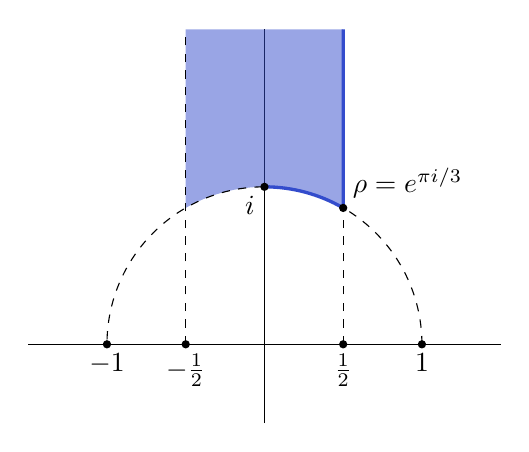
\begin{tikzpicture}
      \draw (-3, 0) -- (3, 0);

      \draw (0, -1) -- (0, 4);

      \node [circ] at (1, 0) {};
      \node [below] at (1, 0) {$\frac{1}{2}$};

      \node [circ] at (2, 0) {};
      \node [below] at (2, 0) {$1$};

      \node [circ] at (-1, 0) {};
      \node [below] at (-1, 0) {$-\frac{1}{2}$};

      \node [circ] at (-2, 0) {};
      \node [below] at (-2, 0) {$-1$};

      \fill [opacity=0.5, mblue] (1, 4) -- (1, 1.732) arc (60:120:2) -- (-1, 4);

      \draw [dashed] (2, 0) arc (0:180:2);

      \draw [dashed] (1, 0) -- (1, 4);
      \draw [dashed] (-1, 0) -- (-1, 4);
      \draw [very thick, mblue] (1, 4) -- (1, 1.732) arc (60:90:2);

      \node [circ] at (1, 1.732) {};
      \node [anchor = south west] at (1, 1.732) {$\rho = e^{\pi i/3}$};
      \node [circ] at (0, 2) {};
      \node [anchor = north east] at (0, 2){$i$};
    \end{tikzpicture}
  \end{center}
  Then $\mathcal{D}$ is a \term{fundamental domain} for the action of $\bar{\Gamma}$ on $\H$, i.e.\ every orbit contains exactly one element of $\mathcal{D}$.

  The stabilizer of $z \in \mathcal{D}$ in $\Gamma$ is trivial if $z \not= i, \rho$, and the stabilizers of $i$ and $\rho$ are
  \[
    \bar{\Gamma}_i = \bra S\ket \cong \frac{\Z}{2Z},\quad \bar\Gamma_\rho = \bra TS\ket \cong \frac{\Z}{3\Z}.
  \]
  Finally, we have $\bar \Gamma = \bra S, T \ket = \bra S, TS\ket$.
\end{thm}
In fact, we have
\[
  \bar \Gamma = \bra S, T \mid S^2 = (TS)^3 = e\ket,
\]
but we will neither prove nor need this.

The proof is rather technical, and involves some significant case work.
\begin{proof}
  Let $\bar{\Gamma}^* = \bra S, T\ket \subseteq \bar{\Gamma}$. We will show that if $z \in \H$, then there exists $\gamma \in \bar\Gamma^*$ such that $\gamma(z) \in \mathcal{D}$.

  Since $z \not \in \R$, we know $\Z + \Z z = \{cz + d: c, d \in \Z\}$ is a discrete subgroup of $\C$. So we know
  \[
    \{|cz + d|: c, d \in \Z\}
  \]
  is a discrete subset of $\R$, and is in particular bounded away from $0$. Thus, we know
  \[
    \left\{\Im \gamma(z) = \frac{\Im (z)}{|cz + d|^2}: \gamma =
    \begin{pmatrix}
      a & b\\
      c & d
    \end{pmatrix} \in \bar\Gamma^*\right\}
  \]
  is a discrete subset of $\R_{>0}$ and is bounded above. Thus there is some $\gamma \in \bar{\Gamma}^*$ with $\Im \gamma(z)$ maximal. Replacing $\gamma$ by $T^n \gamma$ for suitable $n$, we may assume $|\Re \gamma(z)| \leq \frac{1}{2}$.

  We consider the different possible cases.
  \begin{itemize}
    \item If $|\gamma(z)| < 1$, then
      \[
        \Im S \gamma(z) = \Im \frac{-1}{\gamma(z)} = \frac{\Im \gamma(z)}{|\gamma(z)|^2} > \Im \gamma(z),
      \]
      which is impossible. So we know $|\gamma(z)| \geq 1$. So we know $\gamma(z)$ lives in the closure of $\mathcal{D}$.

    \item If $\Re(\gamma(z)) = -\frac{1}{2}$, then $T \gamma(z)$ has real part $+\frac{1}{2}$, and so $T(\gamma(z)) \in \mathcal{D}$.

    \item If $-\frac{1}{2} < \Re(z) < 0$ and $|\gamma(z)| = 1$, then $|S\gamma(z)| = 1$ and $0 < \Re S\gamma(z) < \frac{1}{2}$, i.e.\ $S \gamma(z) \in \mathcal{D}$.
  \end{itemize}
  So we can move it to somewhere in $\mathcal{D}$

  \separator

  We shall next show that if $z, z' \in \mathcal{D}$, and $z' = \gamma(z)$ for $\gamma \in \bar{\Gamma}$, then $z = z'$. Moreover, either
  \begin{itemize}
    \item $\gamma = 1$; or
    \item $z = i$ and $\gamma = S$; or
    \item $z = \rho$ and $\gamma = TS$ or $(TS)^2$.
  \end{itemize}
  It is clear that this proves everything.

  To show this, we wlog
  \[
    \Im (z') = \frac{\Im z}{|cz + d|^2} \geq \Im z
  \]
  where
  \[
    \gamma =
    \begin{pmatrix}
      a & b\\
      c & d
    \end{pmatrix},
  \]
  and we also wlog $c \geq 0$.

  Therefore we know that $|cz + d| \leq 1$. In particular, we know
  \[
    1 \geq \Im(cz + d) = c \Im (z) \geq c \frac{\sqrt{3}}{2}
  \]
  since $z \in \mathcal{D}$. So $c = 0$ or $1$.

  \begin{itemize}
    \item If $c = 0$, then
      \[
        \gamma = \pm
        \begin{pmatrix}
          1 & m\\
          0 & 1
        \end{pmatrix}
      \]
      for some $m \in \Z$, and this $z' = z + m$. But this is clearly impossible. So we must have $m = 0$, $z = z'$, $\gamma = 1 \in \PSL_2(\Z)$.

    \item If $c = 1$, then we know $|z + d| \leq 1$. So $z$ is at distance $1$ from an integer. As $z \in \mathcal{D}$, the only possibilities are $d = 0$ or $-1$.

      \begin{itemize}
        \item If $d = 0$, then we know $|z| = 1$. So
          \[
            \gamma =
            \begin{pmatrix}
              a & -1\\
              1 & 0
            \end{pmatrix}
          \]
          for some $a \in \Z$. Then $z' = a - \frac{1}{z}$. Then
          \begin{itemize}
            \item either $a = 0$, which forces $z = i$, $\gamma = S$; or
            \item $a = 1$, and $z' = 1 - \frac{1}{z}$, which implies $z = z' = \rho$ and $\gamma = TS$.
          \end{itemize}
        \item If $d = -1$, then by looking at the picture, we see that $z = \rho$. Then
          \[
            |cz + d| = |z - 1| = 1,
          \]
          and so
          \[
            \Im z' = \Im z = \frac{\sqrt{3}}{2}.
          \]
          So we have $z' = \rho$ as well. So
          \[
            \frac{a \rho + b}{\rho - 1} = \rho,
          \]
          which implies
          \[
            \rho^2 - (a + 1) \rho - b = 0
          \]
          So $\rho = -1, a = 0$, and $\gamma = (TS)^2$.
      \end{itemize}
  \end{itemize}
\end{proof}
Note that this proof is the same as the proof of reduction theory for binary positive definite binary quadratic forms.

What does the quotient $\bar{\Gamma}\setminus \N$ look like? Each point in the quotient can be identified with an element in $\mathcal{D}$. Moreover, $S$ and $T$ identify the portions of the boundary of $\mathcal{D}$. Thinking hard enough, we see that the quotient space is homeomorphic to a disk.

An important consequence of this is that the quotient $\Gamma \setminus \H$ has \emph{finite invariant measure}.
\begin{prop}
  The measure
  \[
    \d \mu = \frac{\d x\;\d y}{y^2}
  \]
  is invariant under $\PSL_2(\R)$. If $\Gamma \subseteq \PSL_2(\Z)$ is of finite index, then $\mu(\Gamma\setminus \H) < \infty$.
\end{prop}

\begin{proof}
  Consider the $2$-form associated to $\mu$, given by
  \[
    \eta = \frac{\d x \wedge \d y}{y^2} = \frac{i \d z \wedge \d \bar{z}}{2 (\Im z)^2}.
  \]
  We now let
  \[
    \gamma =
    \begin{pmatrix}
      a & b\\
      c & d
    \end{pmatrix} \in \SL_2(\R).
  \]
  Then we have
  \[
    \Im \gamma(z) = \frac{\Im z}{|cz + d|^2}.
  \]
  Moreover, we have
  \[
    \frac{\d \gamma(z)}{\d z} = \frac{a(cz + d) - c(az + b)}{(cz + d)^2} = \frac{1}{(cz + d)^2}.
  \]
  Plugging these into the formula, we see that $\eta$ is invariant under $\gamma$.

  Now if $\bar\Gamma \leq \PSL_2(\Z)$ has finite index, then we can write $\PSL_2(\Z)$ as a union of cosets
  \[
    \PSL_2(\Z) = \coprod_{i = 1}^n \bar\gamma \gamma_i,
  \]
  where $n = (\PSL_2(\Z): \bar\Gamma)$. Then a fundamental domain for $\bar\Gamma$ is just
  \[
    \bigcup_{i = 1}^n \gamma_i(\mathcal{D}),
  \]
  and so
  \[
    \mu(\bar\Gamma \setminus H) = \sum \mu(\gamma_i \mathcal{D}) = n \mu(\mathcal{D}).
  \]
  So it suffices to show that $\mu(\mathcal{D})$ is finite, and we simply compute
  \[
    \mu(\mathcal{D}) = \int_\mathcal{D} \frac{\d x\; \d y}{y^2} \leq \int_{x = -\frac{1}{2}}^{x = \frac{1}{2}}\int_{y = \sqrt{2}/2}^{y = \infty} \frac{\d x\;\d y}{y^2} < \infty.
  \]
\end{proof}
It is an easy exercise to show that we actually have
\[
  \mu(\mathcal{D}) = \frac{\pi}{3}.
\]
We end with a bit terminology.
\begin{defi}[Principal congruence subgroup]\index{$\Gamma(N)$}
  For $N \geq 1$, the \term{principal congruence subgroup}\index{congruence subgroup!principal} of level $N$ is
  \[
    \Gamma(N) = \{\gamma \in \SL_2(\Z) : \gamma \equiv I \pmod N\} = \ker (\SL_2(\Z) \to \SL_2(\Z/N\Z)).
  \]
  Any $\Gamma \subseteq \SL_2(\Z)$ containing some $\Gamma(N)$ is called a \term{congruence subgroup}, and its \term{level} is the smallest $N$ such that $\Gamma \supseteq \Gamma(N)$
\end{defi}

This is a normal subgroup of finite index.
\begin{defi}[$\Gamma_0(N)$, $\Gamma_1(N)$]\index{$\Gamma_0(N)$}\index{$\Gamma_1(N)$}
  We define
  \[
    \Gamma_0(N) =\left\{
      \begin{pmatrix}
        a & b\\
        c & d
      \end{pmatrix}
    \in \SL_2(\Z): c \equiv 0\pmod N\right\}
  \]
  and
  \[
    \Gamma_1(N) =\left\{
      \begin{pmatrix}
        a & b\\
        c & d
      \end{pmatrix}
    \in \SL_2(\Z): c \equiv 0, d\equiv 1 \pmod N\right\}.
  \]
  We similarly define $\Gamma^0(N)$ and $\Gamma^1(N)$ to be the transpose of $\Gamma_0(N)$ and $\Gamma_1(N)$ respectively.
\end{defi}
Note that ``almost all'' subgroups of $\SL_2(\Z)$ are \emph{not} congruence subgroups. On the other hand, if we try to define the notion of congruence subgroups in higher dimensions, we find that all subgroups of $\SL_n(\Z)$ for $n > 2$ are congruence!

\section{Modular forms of level 1}
\subsection{Basic definitions}
We can now define a modular form. Recall that we have $\SL_2(\Z) = \Gamma(1)$.
\begin{defi}[Modular form of level 1]\index{modular form}\index{modular form!level 1}
  A holomorphic function $f: \H \to \C$ is a \emph{modular form of weight $k \in \Z$ and level $1$} if
  \begin{enumerate}
    \item For any
      \[
        \gamma =
        \begin{pmatrix}
          a & b\\
          c & d
        \end{pmatrix} \in \Gamma(1),
      \]
      we have
      \[
        f(\gamma(z)) = (cz + d)^k f(z).
      \]
    \item $f$ is holomorphic at $\infty$ (to be defined precisely later).
  \end{enumerate}
\end{defi}
What can we deduce about modular forms from these properties? If we take $\gamma = -I$, then we get
\[
  f(z) = (-1)^k f(z).
\]
So if $k$ is odd, then $f \equiv 0$. So they only exist for even weights. If we have even weights, then it suffices to consider $\bar{\Gamma} = \bra S, T\ket$. Since
\[
  f(z) \mapsto (cz + d)^{-k} f(\gamma(z))
\]
is a \emph{group action} of $\Gamma(1)$ on functions on $\H$, it suffices to check that $f$ is invariant under the generators $S$ and $T$. Thus, (i) is equivalent to
\[
  f(z + 1) = f(z),\quad f(-1/z) = z^k f(z).
\]
How do we interpret (ii)? We know $f$ is $\Z$-periodic. If we write $q = e^{2\pi i z}$, then we have $z \in \H$ iff $0 < |q| < 1$, and moreover, if two different $z$ give the same $q$, then the values of $f$ on the two $z$ agree. In other words, $f(z)$ only depends on $q$, and thus there exists a holomorphic function $\tilde{f}(q)$ on $\{0< |q| < 1\}$ such that
\[
  \tilde{f}(e^{2\pi i z}) = f(z).
\]
Explicitly, we can write
\[
  \tilde{f}(q) = f\left(\frac{1}{2\pi i} \log q\right).
\]
By definition, $\tilde{f}$ is a holomorphic function on a punctured disk. So we have a Laurent expansion
\[
  \tilde{f}(q) = \sum_{n = -\infty}^\infty a_n (f) q^n,
\]
called the \term{Fourier expansion} or \term{$q$-expansion} of $f$. We say $f$ is meromorphic (resp. holomorphic) at $\infty$ if $\tilde{f}$ is meromorphic (resp. holomorphic) at $q = 0$.

In other words, it is meromorphic at $\infty$ if $a_n(f) = 0$ for $n$ sufficiently negative, and holomorphic if $a_n(f) = 0$ for all $n \geq 0$. The latter just says $f(z)$ is bounded as $\Im(z) \to \infty$.

The following definition is also convenient:
\begin{defi}[Cusp form]\index{cusp form}\index{modular form!cusp form}
  A modular form $f$ is a \emph{cusp form} if the constant term $a_0(f)$ is $0$.
\end{defi}
We will later see that ``almost all'' modular forms are cusp forms.

In this case, we have
\[
  \tilde{f} = \sum_{n\geq 1} a_n(f) q^n.
\]
From now on, we will drop the $\tilde{\;}$, which should not cause confusion.

\begin{defi}[Weak modular form]\index{weak modular form}\index{modular form!weak}
  A \emph{weak modular form} is a holomorphic form on $\H$ satisfying (i) which is \emph{meromorphic} at $\infty$.
\end{defi}
We will use these occasionally.

The transformation rule for modular forms seem rather strong. So, are there actually modular forms? It turns out that there are quite a lot of modular forms, and remarkably, there is a relatively easy way of listing out all the modular forms.

The main class (and in fact, as we will later see, a generating class) of modular forms is due to Eisenstein. This has its origin in the theory of elliptic functions, but we will not go into that.

\begin{defi}[Eisenstein series]\index{Eisenstein series}
  Let $k \geq 4$ be even. We define
  \[
    G_k(z) = \sum_{\substack{m, n \in \Z\\ (m, n) \not= (0, 0)}} \frac{1}{(mz + n)^k} = \sideset{}{'}\sum_{(m, n) \in \Z^2} \frac{1}{(mz + n)^k}.
  \]
\end{defi}
Here the $\sum'$ denotes that we are omitting $0$, and in general, it means we don't sum over things we obviously don't want to sum over.

When we just write down this series, it is not clear that it is a modular form, or even that it converges. This is given by the following theorem:
\begin{thm}
  $G_k$ is a modular form of weight $k$ and level $1$. Moreover, its $q$-expansion is
  \[
    G_k(z) = 2 \zeta(k) \left(1 - \frac{2k}{B_k} \sum_{n \geq 1} \sigma_{k - 1}(n) q^n\right),\tag{$1$}
  \]
  where\index{$\sigma_r(n)$}
  \[
    \sigma_r(n) = \sum_{1 \leq d \mid n} d^r.
  \]
\end{thm}

Convergence of the series follows from the following more general result. Note that since $z \not \in \R$, we know $\{1, z\}$ is an $\R$-basis for $\C$.
\begin{prop}
  Let $(e_1, \cdots, e_d)$ be some basis for $\R^d$. Then if $r \in \R$, the series
  \[
    \sideset{}{'}\sum_{\mathbf{m} \in \Z^d} \|m_1 e_1 + \cdots + m_d e_d\|^{-r}
  \]
  converges iff $r > d$.
\end{prop}

\begin{proof}
  The function
  \[
    (x_i) \in \R^d \mapsto \left\|\sum_{i = 1} x_i e_i \right\|
  \]
  is a norm on $\R^d$. As any $2$ norms on $\R^d$ are equivalent, we know this is equivalent to the sup norm $\|\ph\|_\infty$. So the series converges iff the corresponding series
  \[
    \sum_{\mathbf{m} \in \Z^d}' \|\mathbf{m}\|_\infty^{-r}
  \]
  converges. But if $1 \leq N \leq Z$, then the number of $\mathbf{m} \in \Z^d$ such that $\|\mathbf{m}\|_\infty = N$ is $(2N + 1)^d - (2N - 1)^d \sim 2^d d N^{d - 1}$. So the series converges iff
  \[
    \sum_{N \geq 1} N^{-r} N^{d - 1}
  \]
  converges, which is true iff $r > d$.
\end{proof}

\begin{proof}[Proof of theorem]
  Then convergence of the Eisenstein series by applying this to $\R^2 \cong \C$. So the series is absolutely convergent. Therefore we can simply compute
  \[
    G_k(z + 1) = \sum_{m, n}' \frac{1}{(mz + (m + n))^k} = G_k(z).
  \]
  Also we can compute
  \[
    G_k\left(-\frac{1}{z}\right) = \sum_{m, n}' = \frac{z^k}{(-m + nz)^k} = z^k G_k(z).
  \]
  So $G_k$ satisfies the invariance property. To show that $G_k$ is holomorphic, and holomorphic at infinity, we'll derive the $q$-expansion $(1)$.
\end{proof}

\begin{lemma}
  \[
    \sum_{n = \infty}^\infty \frac{1}{(n + w)^k} = \frac{(-2\pi i)^k}{(k - 1)!} \sum_{d = 1}^\infty d^{k - 1} e^{2\pi i d w}
  \]
  for any $w \in \H$ and $k \geq 2$.
\end{lemma}
There are (at least) two ways to prove this. One of this is to use the series for the cotangent, but here we will use Poisson summation.

\begin{proof}
  Let
  \[
    f(x) = \frac{1}{(x + w)^k}.
  \]
  We compute
  \[
    \hat{f}(y) = \int_{-\infty}^\infty \frac{e^{-2\pi i x y}}{(x + w)^k}\;\d x.
  \]
  We replace this with a contour integral. We see that this has a pole at $-w$. If $y > 0$, then we close the contour downwards, and we have
  \[
    \hat{f}(y) = -2\pi i \Res_{z = -w} \frac{e^{-2\pi i y z}}{(z + w)^k} = -2\pi i \frac{(-2\pi i y)^{k - 1}}{(k - 1)!} e^{2\pi i yw}.
  \]
  If $y \leq 0$, then we close in the upper half plane, and since there is no pole, we have $\hat{f}(y) = 0$. So we have
  \[
    \sum_{n = -\infty}^\infty \frac{1}{(n + w)^k} = \sum_{n \in \Z} f(n) = \sum_{d \in \Z} \hat{f}(d) = \frac{(-2\pi i)^k}{(k - 1)!} \sum_{d \geq 1} d^{k - 1} e^{2\pi i d w}
  \]
  by Poisson summation formula.
\end{proof}

Note that when we proved the Poisson summation formula, we required $f$ to decrease very rapidly at infinity, and our $f$ does not satisfy that condition. However, we can go back and check that the proof still works in this case.

Now we get back to the Eisenstein series. Note that since $k$ is even, we can drop certain annoying signs. We have
\begin{align*}
  G_k(z) &= 2 \sum_{n \geq 1} \frac{1}{n^k} + 2 \sum_{m \geq 1} \sum_{n \in \Z} \frac{1}{(n + mz)^k}\\
  &= 2 \zeta(k) + 2 \sum_{m \geq 1} \frac{(2\pi i )^k}{(k - 1)!} \sum_{d \geq 1} d^{k - 1} q^{dm}.\\
  &= 2 \zeta(k) + 2 \frac{(2\pi i)^k}{(k - 1)!} \sum_{n \geq 1} \sigma_{k - 1}(n) q^n.
\end{align*}
Then the result follows from the fact that
\[
  \zeta(k) = -\frac{1}{2} (2\pi i)^k \frac{B_k}{k!}.
\]
So we see that $G_k$ is holomorphic in $\H$, and is also holomorphic at $\infty$.

It is convenient to introduce a \emph{normalized} Eisenstein series
\begin{defi}[Normalized Eisenstein series]\index{normalized Eisenstein series}\index{Eisenstein series!normalized}
  We define
  \begin{align*}
    E_k(z) &= (2 \zeta(k))^{-1} G_k(z) \\
    &= 1 - \frac{2k}{B_k} \sum_{n \geq 1} \sigma_{k - 1}(n) q^n\\
    &= \frac{1}{2} \sum_{\substack{(m, n) = 1\\m , n \in \Z}} \frac{1}{(mz + n)^k}.
  \end{align*}
\end{defi}
The last line follows by taking out any common factor of $m, n$ in the series defining $G_k$.

Thus, to figure out the (normalized) Eisenstein series, we only need to know the Bernoulli numbers.
\begin{eg}
  We have
  \begin{align*}
    B_2 &= \frac{1}{6}, & B_4 &= \frac{-1}{30}, & B_6 &= \frac{1}{42}, & B_8 &= \frac{-1}{30}\\
    B_{10} &= \frac{5}{66}, & B_{12} &= \frac{-631}{2730}, & B_{14} &= \frac{7}{6}.
  \end{align*}
  Using these, we find
  \begin{align*}
    E_4 &= 1 + 240 \sum \sigma_3(n) q^n\\
    E_6 &= 1 - 504 \sum \sigma_5 (n) q^n\\
    E_8 &= 1 + 480 \sum \sigma_7(n) q^n\\
    E_{10} &= 1 - 264 \sum \sigma_9(n) q^n\\
    E_{12} &= 1 + \frac{65520}{691} \sum \sigma_{11}(n) q^n\\
    E_{14} &= 1 - 24 \sum \sigma_{13}(n) q^n.
  \end{align*}
\end{eg}
We notice that there is a simple pattern for $k \leq 14$, except for $k = 12$.

For more general analysis of modular forms, it is convenient to consider the following notation:
\begin{defi}[Slash operator]\index{slash operator}
  Let
  \[
    \begin{pmatrix}
      a & b\\
      c & d
    \end{pmatrix} = \gamma \in \GL_2(\R)^+,\quad z \in \H,
  \]
  and $f: \H \to \C$ any function. We write\index{$j(\gamma, z)$}\index{$f\underset{k}{|}\gamma$}
  \[
    j(\gamma, z) = cz + d.
  \]
  We define the \emph{slash operator} to be
  \[
    (f\underset{k}{|} \gamma) (z) = (\det \gamma)^{k/2} j(\gamma, z)^{-k} f(\gamma(z)).
  \]
\end{defi}
Note that some people leave out the $\det \gamma^{k/2}$ factor, but if we have it, then whenever $\gamma = Ia$, then
\[
  f\underset{k}{|} \gamma = \sgn(a)^k f,
\]
which is annoying. In this notation, then condition (i) for $f$ to be a modular form is just
\[
  f\underset{k}{|}\gamma = f
\]
for all $\gamma \in \SL_2(\Z)$.

To prove things about our $j$ operator, it is convenient to note that
\[
  \gamma
  \begin{pmatrix}
    z\\1
  \end{pmatrix}
  = j(\gamma, z)
  \begin{pmatrix}
    \gamma(z)\\1
  \end{pmatrix}.\tag{$*$}
\]
\begin{prop}\leavevmode
  \begin{enumerate}
    \item $j(\gamma\delta, z) = j(\gamma, \delta(z)) j(\delta, z)$ (in fancy language, we say $j$ is a 1-cocycle).
    \item $j(\gamma^{-1}, z) = j (\gamma, \gamma^{-1}(z))^{-1}$.
    \item $\gamma: \varphi \mapsto f\underset{k}{|} \gamma$ is a (right) action of $G = \GL_2(\R)^+$ on functions on $\H$. In other words,
      \[
        f\underset{k}{|} \gamma \underset{k}{|} \delta = f\underset{k}{|}(\gamma\delta).
      \]
  \end{enumerate}
\end{prop}
Note that this implies that if if $\Gamma \leq \GL_2(\R)^+$ and $\Gamma = \bra \gamma_1, \cdots, \gamma_m\ket$ then
\[
  f\underset{k}{|} \gamma = f\Longleftrightarrow f\underset{k}{|} \gamma_i = f\text{ for all }i = 1, \cdots, m.
\]
The proof is just a computation.
\begin{proof}\leavevmode
  \begin{enumerate}
    \item We have
      \[
        j(\gamma\delta, z)
        \begin{pmatrix}
          \gamma\delta(z)\\
          1
        \end{pmatrix} =
        \gamma\delta
        \begin{pmatrix}
          z\\1
        \end{pmatrix}
        =
        j(\delta, z) \gamma
        \begin{pmatrix}
          \delta(z)\\
          1
        \end{pmatrix}
        =
        j(\delta, z) j(\gamma, \delta(z))
        \begin{pmatrix}
          z\\1
        \end{pmatrix}
      \]
    \item Take $\delta = \gamma^{-1}$.
    \item We have
      \begin{align*}
        ((f\underset{k}{|} \gamma) \underset{k}{|} \delta)(z) &= (\det \delta)^{k/2} j(\delta, z)^{-k} (f\underset{k}{|} \gamma) (\delta(z))\\
        &= (\det \delta)^{k/2} j(\delta, z)^{-k} (\det \gamma)^{k/2} j(\gamma, \delta(z))^{-k} f(\gamma\delta(z))\\
        &= (\det \gamma \delta)^{k/2} j(\gamma \delta, z)^{-k} f(\gamma\delta(z))\\
        &= (f\underset{k}{|} \gamma\delta) (z).
      \end{align*}
  \end{enumerate}
\end{proof}
Back to the Eisenstein series. $G_k$ arise naturally in elliptic functions, which are coefficients in the series expansion of Weierstrass $\wp$ function.

There is another group-theoretic interpretation, which generalizes in many ways. Consider
\[
  \Gamma(1)_\infty = \left\{
    \pm
    \begin{pmatrix}
      1 & n\\
      0 & 1
    \end{pmatrix}: n \in \Z
  \right\} \leq \Gamma(1) = \SL_2(\Z),
\]
which is the stabilizer of $\infty$. If
\[
  \delta = \pm
  \begin{pmatrix}
    1 & n\\
    0 & 1
  \end{pmatrix}
  \in \Gamma(1)_\infty,
\]
then we have
\[
  j(\delta\gamma, z) = j(\delta, \gamma(z)) j(\gamma, z) = \pm j(\gamma, z).
\]
So $j(\gamma, z)^2$ depends only on the coset $\Gamma(1)_\infty \gamma$. We can also check that if
\[
  \gamma =
  \begin{pmatrix}
    a & b\\
    c & d
  \end{pmatrix},\quad
  \gamma =
  \begin{pmatrix}
    a' & b'\\
    c' & d'
  \end{pmatrix} \in \Gamma(1),
\]
then $\Gamma(1)_\infty \gamma = \Gamma(1)_\infty \gamma'$ iff $(c, d) = \pm (c', d')$.

Moreover, $\gcd(c, d) = 1 $ iff there exists $a, b$ such that
\[
  \begin{vmatrix}
    a & b\\
    c & d
  \end{vmatrix} = 1.
\]
We therefore have
\[
  E_k(z) = \sum_{\gamma \in \Gamma(1)_\infty \setminus \Gamma(1)} j(\gamma, z)^{-k},
\]
where we sum over (any) coset representatives of $\Gamma(1)_\infty$.

We can generalize this in two ways. We can either replace $j$ with some other appropriate function, or change the groups.

\subsection{The space of modular forms}
In this section, we are going to find out \emph{all} modular forms! For $k \in \Z$, we write $M_k = M_k(\Gamma(1))$\index{$M_k$}\index{$M_k(\Gamma(1))$} for the set of modular forms of weight $k$ (and level $1$). We have $S_k \subseteq S_k(\Gamma(1))$\index{$S_k$}\index{$S_k(\Gamma)$} containing the cusp forms. These are $\C$-vector spaces, and are zero for odd $k$.

Moreover, from the definition, we have a natural product
\[
  M_k \cdot M_\ell \subseteq M_{k + \ell}.
\]
Likewise, we have
\[
  S_k\cdot M_\ell \subseteq S_{k + \ell}.
\]
We let\index{$M_*$}\index{$S_*$}
\[
  M_* = \bigoplus_{k \in \Z} M_k,\quad S_* = \bigoplus_{k \in \Z} S_k.
\]
Then $M_*$ is a graded ring and $S_*$ is a graded ideal. By definition, we have
\[
  S_k = \ker (a_0: M_k \to \C).
\]
To figure out what all the modular forms are, we use the following constraints on the zeroes of a modular form:

\begin{prop}
  Let $f$ be a weak modular form (i.e.\ it can be meromorphic at $\infty$) of weight $k$ and level $1$. Then $f$ is not identically zero, then
  \[
    \left(\sum_{z_0 \in \mathcal{D} \setminus \{i, \rho\}} \ord_{z_0} (f)\right) + \frac{1}{2} \ord_i(f) + \frac{1}{3} \ord_\rho f + \ord_\infty(f) = \frac{k}{12},
  \]
  where $\ord_\infty f$ is the least $r \in \Z$ such that $a_r(f) \not= 0$.
\end{prop}
Note that if $\gamma \in \Gamma(1)$, then $j(\gamma, z) = cz + d$ is never $0$ for $z \in \H$. So it follows that $\ord_z f = \ord_{\gamma(z)} f$.

We will prove this using the argument principle.
\begin{proof}
  Note that the function $\tilde{f}(q)$ is non-zero for $0 < |q| < \varepsilon$ for some small $\varepsilon$ by the principle of isolated zeroes. Setting
  \[
    \varepsilon = e^{-2\pi R},
  \]
  we know $f(z) \not= 0$ if $\Im z \geq R$.

  In particular, the number of zeroes of $f$ in $\mathcal{D}$ is finite. We consider the integral along the following contour, counterclockwise.
  \begin{center}
    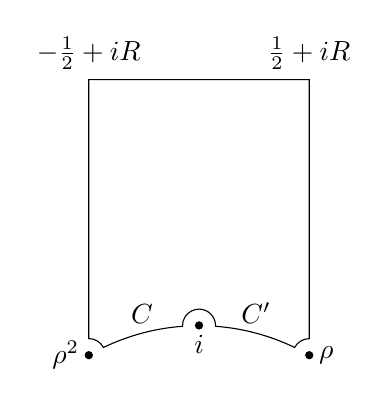
\begin{tikzpicture}[scale=0.7]
% \draw [gray] (-2, -5) -- (-2, 1) -- (2, 1) -- (2, -5);
% \draw [gray] (0, -7.46) circle [radius=4];
% \draw [gray] (2, -4) circle [radius=0.3];
% \draw [gray] (-2, -4) circle [radius=0.3];
% \draw [gray] (0, -3.46) circle [radius=0.3];
% \draw (-1, 2) -- (1, 2) -- (1, -1.5) arc(90:164.48:0.5) arc(88.96:90:1);

      \node [circ] at (2, -4) {};
      \node [right] at (2, -4) {$\rho$};
      \node [circ] at (-2, -4) {};
      \node [left] at (-2, -4) {$\rho^2$};
      \node [circ] at (0, -3.46) {};
      \node [below] at (0, -3.46) {$i$};

      \node [above] at (2, 1) {$\frac{1}{2} + iR$};
      \node [above] at (-2, 1) {$-\frac{1}{2} + iR$};
      \draw (-2, 1) -- (2, 1) -- (2, -3.7) arc(90:152.15:0.3) arc(64.298:85.7018:4) node [pos=0.5, above] {$C'$} arc(-2.149:182.149:0.3) arc(94.2982:115.702:4) node [pos=0.5, above] {$C$} arc(27.5:90:0.3) -- cycle;;
    \end{tikzpicture}
  \end{center}
  We assume $f$ has no zeroes along the contour. Otherwise, we need to go around the poles, which is a rather standard complex analytic maneuver we will not go through.

  For $\varepsilon$ sufficiently small, we have
  \[
    \int_\Gamma \frac{f'(z)}{f(z)}\;\d z = 2\pi i \sum_{z_0 \in \mathcal{D} \setminus \{i, \rho\}} \ord_{z_0 f}
  \]
  by the argument principle. Now the top integral is
  \[
    \int_{\frac{1}{2} + iR}^{-\frac{1}{2} iR} \frac{f'}{f}\;\d z = -\int_{|q| = \varepsilon} \frac{\frac{\d \tilde{f}}{\d q}}{\tilde{f}(q)} \;\d q = -2\pi i \ord_{\infty} f.
  \]
  As $\frac{f'}{f}$ has at worst a simple pole at $z = i$, the residue is $\ord_i f$. Since we are integrating along only half the circle, as $\varepsilon \to 0$, we pick up
  \[
    - \pi i \res = - \pi i \ord_i f.
  \]
  Similarly, we get $-\frac{2}{3} \pi i \ord_\rho f$ coming from $\rho$ and $\rho^2$.

  So it remains to integrate along the bottom circular arcs. Now note that $S: z \mapsto -\frac{1}{z}$ maps $C$ to $C'$ with opposite orientation, and
  \[
    \frac{\d f(Sz)}{f(Sz)} = k \frac{\d z}{z} + \frac{\d f(z)}{f(z)}
  \]
  as
  \[
    f(Sz) = z^k f(z).
  \]
  So we have
  \begin{align*}
    \int_C + \int_{C'} \frac{f'}{f}\;\d z &= \int_{C'} \frac{f'}{f}\;\d z - \left(\frac{k}{z} \;\d z + \frac{f'}{f}\;\d z\right) - -k \int_{C'} \frac{\d z}{z}\\
    &\to k \int_\rho^i \frac{\d z}{z} \\
    &= \frac{\pi i k}{6}.
  \end{align*}
  So taking the limit $\varepsilon \to 0$ gives the right result.
\end{proof}

\begin{cor}
  If $k < 0$, then $M_k = \{0\}$.
\end{cor}

\begin{cor}
  If $k = 0$, then $M_0 = \C$, the constants, and $S_0 = \{0\}$.
\end{cor}

\begin{proof}
  If $f \in M_0$, then $g = f - f(1)$. If $f$ is not constant, then $\ord_i g \geq 1$, so the LHS is $>0$, but the RHS is $=0$. So $f \in \C$.

  Of course, $a_0(f) = f$. So $S_0 = \{0\}$.
\end{proof}

\begin{cor}
  \[
    \dim M_k \leq 1 + \frac{k}{12}.
  \]
  In particular, they are finite dimensional.
\end{cor}

\begin{proof}
  We let $f_0, \cdots, f_d$ be $d + 1$ elements of $M_k$, and we choose distinct points $z_1, \cdots, z_d \in \mathcal{D} \setminus \{i, \rho\}$. Then there exists $\lambda_0, \cdots, \lambda_d \in \C$, not all $0$, such that
  \[
    f = \sum_{i = 0}^d \lambda_i f_i
  \]
  vanishes at all these points. Now if $d > \frac{k}{12}$, then LHS is $> \frac{k}{12}$. So $f \equiv 0$. So $(f_i)$ are linearly dependent, i.e.\ $\dim M_k < d + 1$.
\end{proof}

\begin{cor}\leavevmode
  $M_2 = \{0\}$ and $M_k = \C E_k$ for $4 \leq k \leq 10$ ($k$ even). We also have $E_8 = E_4^2$ and $E_{10} = E_4 E_6$.
\end{cor}

\begin{proof}
  Only $M_2 = \{0\}$ requires proof. If $0 \not= f \in M_2$, then this implies
  \[
    a + \frac{b}{2} + \frac{c}{3} = \frac{1}{6}
  \]
  for integers $a, b, c \geq 0$, which is not possible.

  Alternatively, if $f \in M_2$, then $f^2 \in M_4$ and $f^3 \in M_6$. This implies $E_4^3 = E_6^2$, which is not the case as we will soon see.

  Note that we know $E_8 = E_4^2$, and is not just a multiple of it, by checking the leading coefficient (namely 1).
\end{proof}

\begin{cor}
  The cusp form of weight $12$ is
  \[
    E_4^3 - E_6^2 = (1 + 240 q + \cdots)^3 - (1 - 504 q + \cdots)^2 = 1728q + \cdots.
  \]
\end{cor}
Note that $1728 = 12^3$.

\begin{defi}[$\Delta$ and $\tau$]\index{$\Delta$}\index{$\tau(n)$}
  \[
    \Delta = \frac{E_4^3 - E_6^2}{1728} = \sum_{n \geq 1} \tau(n) q^n \in S_{12}.
  \]
\end{defi}
This function $\tau$ is very interesting, and is called \term{Ramanujan's $\tau$-function}. It has nice arithmetic properties we'll talk about soon.

The following is a crucial property of $\Delta$:
\begin{prop}
  $\Delta(z) \not= 0$ for all $z \in \H$.
\end{prop}

\begin{proof}
  We have
  \[
    \sum_{z_0 \not= i, \rho} \ord_{z_0} \Delta + \frac{1}{2} \ord_i \Delta + \frac{1}{3} \ord_\rho \Delta + \ord_\infty \Delta = \frac{k}{12} = 1.
  \]
  Since $\ord_\rho \Delta = 1$, it follows that there can't be any other zeroes.
\end{proof}

It follows from this that
\begin{prop}
  The map $f \mapsto \Delta f$ is an isomorphism $M_{k - 12}(\Gamma(1)) \to S_k(\Gamma(1))$ for all $k > 12$.
\end{prop}

\begin{proof}
  Since $\Delta \in S_{12}$, it follows that if $f \in M_{k - 1}$, then $\Delta f \in S_k$. So the map is well-defined, and we certainly get an injection $M_{k - 12} \to S_k$. Now if $g \in S_k$, since $\ord_\infty \Delta = 1 \leq \ord_\infty g$ and $\Delta \not= \H$. So $\frac{g}{\Delta}$ is a modular form of weight $k - 12$.
\end{proof}

Thus, we find that
\begin{thm}\leavevmode
  \begin{enumerate}
    \item We have
      \[
        \dim M_k (\Gamma(1)) =
        \begin{cases}
          0 & k < 0\text{ or }k \text{ odd }\\
          \left\lfloor \frac{k}{12}\right\rfloor & k > 0, k \equiv 2 \pmod{12}\\
          1 + \left\lfloor \frac{k}{12}\right\rfloor & \text{otherwise}
        \end{cases}
      \]
    \item If $k > 4$ and even, then
      \[
        M_k = S_k \oplus \C E_k.
      \]
    \item Every element of $M_k$ is a polynomial in $E_4$ and $E_6$.
    \item Let
      \[
        b =
        \begin{cases}
          0 & k\equiv 0 \pmod 4\\
          1 & k\equiv 2 \pmod 4
        \end{cases}.
      \]
      Then
      \[
        \{h_j = \Delta^j E_6^b E_4^{(k - 12j - 6b)/4} : 0 \leq j < \dim M_k\}.
      \]
      is a basis for $M_k$, and
      \[
        \{h_j : 1 \leq j < \dim M_k\}
      \]
      is a basis for $S_k$.
  \end{enumerate}
\end{thm}
\begin{proof}\leavevmode
  \begin{enumerate}
    \item[(ii)] $S_k$ is the kernel of the homomorphism $M_k \to \C$ sending $f \mapsto a_0(f)$. So the complement of $S_k$ has dimension at most $1$, and we know $E_k$ is an element of it. So we are done.
    \item[(i)] For $k < 12$, this agrees with what we have already proved. By the proposition, we have
      \[
        \dim M_{k - 12} = \dim S_k.
      \]
      So we are done by induction and (ii).
    \item[(iii)] This is true for $k < 12$. If $k \geq 12$ is even, then we can find $a, b \geq 0$ with $4a + 6b = k$. Then $E_4^a E_6^b \in M_k$, and is not a cusp form. So
      \[
        M_k = \C E_4^a E_6^b \oplus \Delta M_{k - 12}.
      \]
      But $\Delta$ is a polynomial in $E_4, E_6$, So we are done by induction on $k$.
    \item[(iv)] By (i), we know $k - 12j - 6k \geq 0$ for $j < \dim M_k$, and is a multiple of $4$. So $h_j \in M_k$. Next note that the $q$-expansion of $h_j$ begins with $q^j$. So they are all linearly independent.\qedhere
  \end{enumerate}
\end{proof}
So we have completely determined all modular forms, and this is the end of the course.

\newpage
\subsection{Arithmetic of \tph{$\Delta$}{Delta}{&Delta;}}
Recall that we had
\[
  \Delta = \sum \tau(n) q^n,
\]
and we knew
\[
  \tau(1) = 1,\quad \tau(n) \in \Q.
\]
In fact, more is true.
\begin{prop}\leavevmode
  \begin{enumerate}
    \item $\tau(n) \in \Z$ for all $n \geq 1$.
    \item $\tau(n) = \sigma_{11}(n) \pmod {691}$
  \end{enumerate}
\end{prop}
The function $\tau$ satisfies many more equations, some of which are on the second example sheet.

\begin{proof}\leavevmode
  \begin{enumerate}
    \item We have
      \[
        1728 \Delta = (1 + 240 A_3(q))^3 - (1 - 504 A_5 (q))^2,
      \]
      where
      \[
        A_r = \sum_{n \geq 1} \sigma_r(n) q^n.
      \]
      We can write this as
      \[
         1728\Delta = 3\cdot 240 A_3 + 3\cdot 240^2 A_3^2 + 240^3 A_3^3 + 2\cdot 504 A_5 - 504^2 A_5^2.
      \]
      Now recall the deep fact that $1728 = 12^3$ and $504 = 21 \cdot 24$.

      Modulo 1728, this is equal to
      \[
        720 A_3 + 1008 A_5.
      \]
      So it suffices to show that
      \[
        5 \sigma_3 + 7 \sigma_5(n) \equiv 0 \pmod {12}.
      \]
      In other words, we need
      \[
        5 d^3 + 7 d^5 \equiv 0 \pmod {12},
      \]
      and we can just check this manually for all $d$.
    \item Consider
      \[
        E_4^3 = 1 + \sum_{n \geq 1} b_n q^n
      \]
      with $b_n \in \Z$. We also have
      \[
        E_{12} = 1 + \frac{65520}{691} \sum_{n \geq 1} \sigma_{11}(n) q^n.
      \]
      Also, we know
      \[
        E_{12} - E_4^3 \in S_{12}.
      \]
      So it is equal to $\lambda \Delta$ for some $\lambda \in \Q$. So we find that for all $n \geq 1$, we have
      \[
        \frac{665520}{691} \sigma_{11}(n) - b_n = \lambda \tau(n).
      \]
      In other words,
      \[
        65520 \sigma_{11}(n) - 691 b_n = \mu \tau(n)
      \]
      for some $\tau \in \Q$.

      Putting $n = 1$, we know $\tau(1) = 1$, $\sigma_{11}(1) = 1$, and $b_1 \in \Z$. So $\mu \in \Z$ and $\mu \equiv 65520 \pmod {691}$. So for all $n \geq 1$, we have
      \[
        65520 \sigma_{11}(n) \equiv 65520 \tau(n) \pmod {691}.
      \]
      Since $691$ and $65520$ are coprime, we are done.
  \end{enumerate}
\end{proof}
This proof is elementary, once we had the structure theorem, but doesn't really explain \emph{why} the congruence is true.

The function $\tau(n)$ was studied extensively by Ramanujan. He proved the $691$ congruence (and many others), and (experimentally) observed that if $(m, n) = 1$, then
\[
  \tau(mn) = \tau(m) \tau(n).
\]
Also, he observed that for any prime $p$, we have
\[
  |\tau(p)| < 2 p^{11/2},
\]
which was a rather curious thing to notice. Both of these things are true, and we will soon prove that the first is true. The second is also true, but it uses deep algebraic geometry. It was proved by Deligne in 1972, and he got a fields medal for proving this. So it's pretty hard.

We will also prove a theorem of Jacobi:
\[
  \Delta = q \prod_{n = 1}^{\infty} (1 - q^n)^{24}.
\]
The numbers $\tau(p)$ are related to \emph{Galois representations}.

\subsubsection*{Rationality and integrality}
So far, we have many series that have rational coefficients in them. Given any subring $R \subseteq \C$, we let $M_k(R) = M_k(\Gamma(1), R)$ be the set of all $f \in M_k$ such that all $a_n(f) \in R$. Likewise, we define $S_k(R)$. For future convenience, we will prove a short lemma about them.

\begin{lemma}\leavevmode
  \begin{enumerate}
    \item Suppose $\dim M_k = d + 1 \geq 1$. Then there exists a basis $\{g_j: 0 \leq j \leq d\}$ for $M_k$ such that
      \begin{itemize}
        \item $g_j \in M_k(\Z)$ for all $j \in \{0, \cdots, d\}$.
        \item $a_n(g_j) = \delta_{nj}$ for all $j, n \in \{0, \cdots, d\}$.
      \end{itemize}
    \item For any $R$, $M_k(R) \cong R^{d + 1}$ generated by $\{g_j\}$.
  \end{enumerate}
\end{lemma}

\begin{proof}\leavevmode
  \begin{enumerate}
    \item We take our previous basis $h_j = \Delta^j E_6^b E_4^{(k - 12j - 6b)/4} \in M_k(\Z)$. Then we have $a_n(h_n) = 1$, and $a_j(h_n) = 0$ for all $j < n$. Then we just row reduce.
    \item The isomorphism is given by
      \[
        \begin{tikzcd}[cdmap]
          M_k(R) \ar[r, leftrightarrow] & R^{d + 1}\\
          f \ar[r, maps to] & (a_n(f))\\
          \displaystyle \sum_{j = 0}^d c_j g_j & (c_n) \ar[l, maps to]
        \end{tikzcd}
      \]
  \end{enumerate}
\end{proof}

\section{Hecke operators}
\subsection{Hecke operators and algebras}
Recall that for $f: \H \to \C$, $\gamma \in \GL_2(\R)^+$ and $k \in \Z$, we defined
\[
  (f\underset{k}{|} \gamma)(z) = (\det \gamma)^{k/2} j(\gamma, z)^k f(\gamma(z)),
\]
where
\[
  \gamma =
  \begin{pmatrix}
    a & b\\
    c & d
  \end{pmatrix},\quad j(\gamma, z) = cz + d.
\]
We then defined
\[
  M_k = \{f: f \underset{k}{|} \gamma = f\text{ for all }\gamma \in \Gamma(1) + \text{holomorphicity condition}\}.
\]
We showed that these are finite-dimensional, and we found a basis. But there is more to be said about modular forms. Just because we know polynomials have a basis $1, x, x^2, \cdots$ does not mean there isn't anything else to say about polynomials!

In this chapter, we will figure that $M_k$ has the structure of a module for the \emph{Hecke algebra}. This structure underlies the connection with arithmetic, i.e.\ Galois representations etc.

How might we try to get some extra structure on $M_k$? We might try to see what happens if we let something else in $\GL_2(\R)^+$ act on $f$. Unfortunately, in general, if $f$ is a modular form and $\gamma \in \GL_2(\R)^+$, then $g = f \underset{k}{|} \gamma$ is not a modular form. Indeed, given a $\delta\in \Gamma(1)$, then it acts on $g$ by
\[
  g\underset{k}{|} \delta = f\underset{k}{|} \gamma\delta = (f\underset{k}{|} \gamma \delta \gamma^{-1})\gamma
\]
and usually $\gamma \delta \gamma^{-1} \not \in \Gamma(1)$. In fact the normalizer of $\Gamma(1)$ in $\GL_2(\R)^+$ is generated by $\Gamma(1)$ and $aI$ for $a \in \R^*$.

It turns out we need to act in a smarter way. To do so, we have to develop quite a lot of rather elementary group theory.

%\begin{lemma}
% Let $G$ be a group and $\Gamma, \Gamma' \leq G$ be subgroups. We further suppose $\Gamma$ has finite index, and let $\Gamma \gamma_1, \cdots, \Gamma \gamma_n$ be the cosets. Also, we suppose $\Gamma'$ permutes the cosets of $\Gamma$ when acting by right multiplication.
%
% Let $M$ be a $G$-module, and let $f \in M^\Gamma$. We define
% \[
% g = \sum_{i = 1}^n f \gamma_i.
% \]
% Then $g \in \Gamma'$, and does not depend on the choice of the $\gamma_i$.
%\end{lemma}
%
%\begin{proof}
% If $\Gamma \gamma_i = \Gamma \gamma_i'$, then there are some $h_i \in \Gamma$ such that $\gamma_i = h \gamma_i'$. Then
% \[
% g = \sum f \gamma_i = \sum f h_i \gamma_i' = \sum f \gamma_i'
% \]
% since $f \in M^\Gamma$. So $g$ does not depend on the choice of the $\gamma_i$.
%
% Now let $\delta \in \Gamma'$. By hypothesis, there exists $\pi \in S_n$ and $\varepsilon_i \in \Gamma$ for $i = 1,\cdots, n$ such that
% \[
% \Gamma \gamma_i \delta = \Gamma \gamma_{\pi(i)},\quad \gamma_{\pi(i)} = \varepsilon_i \gamma_i \delta.
% \]
% Then we have
% \[
% g \delta = \sum f \gamma_i \delta = \sum f \varepsilon_i ^{-1} \gamma_{\pi(i)} = \sum f \gamma_{\pi(i)} = g,
% \]
% since $\varepsilon_i^{-1} \in \Gamma$.
%\end{proof}
Consider a group $G$, and $\Gamma \leq G$. The idea is to use the \term{double cosets} of $\Gamma$ defined by
\[
  \Gamma g \Gamma = \{\gamma g \gamma' : \gamma, \gamma' \in \Gamma\}.
\]
One alternative way to view this is to consider the right multiplication action of $G$, hence $\Gamma$ on the right cosets $\Gamma g$. Then the double coset $\Gamma g \Gamma$ is the union of the orbits of $\Gamma g$ under the action of $\Gamma$. We can write this as
\[
  \Gamma g \Gamma = \coprod_{i \in I} \Gamma g_i
\]
for some $g_i \in g\Gamma \subseteq G$ and index set $I$.

In our applications, we will want this disjoint union to be finite. By the orbit-stabilizer theorem, the size of this orbit is the index of the stabilizer of $\Gamma g$ in $\Gamma$. It is not hard to see that the stabilizer is given by $\Gamma \cap g^{-1} \Gamma g$. Thus, we are led to consider the following hypothesis:
\begin{center}
  \textbf{Hypothesis (H)}: For all $g \in G$, $(\Gamma: \Gamma \cap g^{-1} \Gamma g) < \infty$.
\end{center}
Then $(G, \Gamma)$ satisfies (H) iff for any $g$, the double coset $\Gamma g \Gamma$ is the union of finitely many cosets.

The important example is the following:
\begin{thm}
  Let $G = \GL_2(\Q)$, and $\Gamma \subseteq \SL_2(\Z)$ a subgroup of finite index. Then $(G, \Gamma)$ satisfies (H).
\end{thm}

\begin{proof}
  We first consider the case $\Gamma = \SL_2(\Z)$. We first suppose
  \[
    g =
    \begin{pmatrix}
      a & b\\
      c & d
    \end{pmatrix}
    \in \Mat_2(\Z),
  \]
  and $\det g = \pm N$, $N \geq 1$. We claim that
    \[
    g^{-1}\Gamma g \cap \Gamma \supseteq \Gamma(N),
  \]
  from which it follows that
  \[
    (\Gamma : \Gamma \cap g^{-1} \Gamma g) < \infty.
  \]
  So given $\gamma \in \Gamma(N)$, we need to show that $g \gamma g^{-1} \in \Gamma$, i.e.\ it has integer coefficients. We consider
  \[
    \pm N \cdot g \gamma g^{-1} =
    \begin{pmatrix}
      a & b\\
      c & d
    \end{pmatrix} \gamma
    \begin{pmatrix}
      d & -b\\
      -c& a
    \end{pmatrix}
    \equiv
    \begin{pmatrix}
      a & b\\
      c & d
    \end{pmatrix}
    \begin{pmatrix}
      d & -b\\
      -c & a
    \end{pmatrix} \equiv NI \equiv 0\pmod N.
  \]
  So we know that $g \gamma g^{-1}$ must have integer entries. Now in general, if $g' \in \GL_2(\Q)$, then we can write
  \[
    g' = \frac{1}{M} g
  \]
  for $g$ with integer entries, and we know conjugating by $g$ and $g'$ give the same result. So $(G, \Gamma)$ satisfies (H).

  \separator

  The general result follows by a butterfly. Recall that if $(G: H) < \infty$ and $(G: H') < \infty$, then $(G: H \cap H') < \infty$. Now if $\Gamma \subseteq \Gamma(1) = \SL_2(\Z)$ is of finite index, then we can draw the diagram
  \begin{center}
    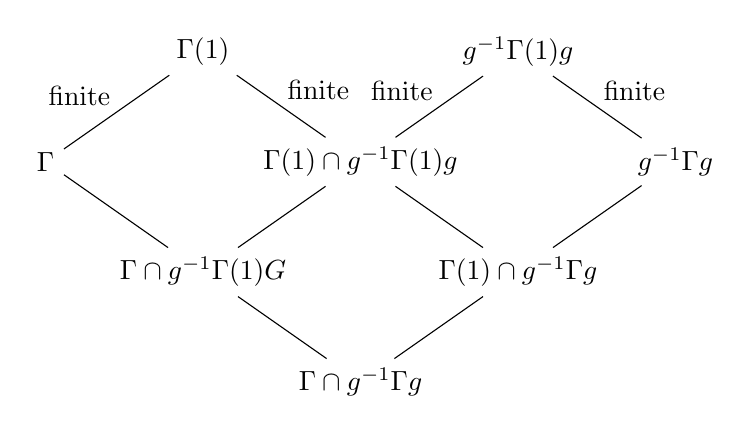
\begin{tikzpicture}[yscale=0.7, commutative diagrams/every diagram]
      \node (12) at (0, 0) {$\Gamma(1)$}; \node (14) at (4, 0) {$g^{-1}\Gamma(1)g$};
      \node (21) at (-2, -2) {$\Gamma$}; \node (23) at (2, -2) {$\Gamma(1) \cap g^{-1}\Gamma(1) g$}; \node (25) at (6, -2) {$g^{-1}\Gamma g$};
      \node (32) at (0, -4) {$\Gamma \cap g^{-1} \Gamma(1)G$}; \node (34) at (4, -4) {$\Gamma(1) \cap g^{-1} \Gamma g$};
      \node (43) at (2, -6) {$\Gamma \cap g^{-1} \Gamma g$};

      \path [commutative diagrams/.cd, every arrow, every label, dash]
      (12) edge node [swap] {finite} (21)
      (12) edge node {finite} (23)
      (14) edge node [swap] {finite} (23)
      (14) edge node {finite} (25)
      (21) edge (32)
      (23) edge (32)
      (23) edge (34)
      (25) edge (34)
      (32) edge (43)
      (34) edge (43);
    \end{tikzpicture}
  \end{center}
  Each group is the intersection of the two above, and so all inclusions are of finite index.
\end{proof}
Note that the same proof works for $\GL_N(\Q)$ for any $N$.

Before we delve into concreteness, we talk a bit more about double cosets. Recall that cosets partition the group into pieces of equal size. Is this true for double cosets as well? We can characterize double cosets as orbits of $\Gamma \times \Gamma$ acting on $G$ by
\[
  (\gamma, \delta) \cdot g = \gamma g \delta^{-1}.
\]
So $G$ is indeed the disjoint union of the double cosets of $\Gamma$.

However, it is not necessarily the case that all double cosets have the same size. For example $|\Gamma e \Gamma| = |\Gamma|$, but for a general $g$, $|\Gamma g \Gamma|$ can be the union of many cosets of $\Gamma$.

Our aim is to define a ring $\mathcal{H}(G, \Gamma)$ generated by double cosets called the \emph{Hecke algebra}. As an abelian group, it is the free abelian group on symbols $[\Gamma g\Gamma]$ for each double coset $[\Gamma g \Gamma]$. It turns out instead of trying to define a multiplication for the Hecke algebra directly, we instead try to define an action of this on interesting objects, and then there is a unique way of giving $\mathcal{H}(G, \Gamma)$ a multiplicative structure such that this is a genuine action.

Given a group $G$, a \term{$G$-module} is an abelian group with a $\Z$-linear $G$-action. In other words, it is a module of the group ring $\Z G$. We will work with right modules, instead of the usual left modules.

Given such a module and a subgroup $\Gamma \leq G$, we will write
\[
  M^\Gamma = \{m \in M : m \gamma = m \text{ for all } \gamma \in \Gamma\}.
\]
\begin{notation}
  For $g \in G$ and $m \in M^\Gamma$, we let
  \[
    m|[\Gamma g \Gamma] = \sum_{i = 1}^n m g_i,\tag{$*$}
  \]
  where
  \[
    \Gamma g \Gamma = \coprod_{i = 1}^n \Gamma g_i.
  \]
\end{notation}
The following properties are immediate, but also crucial.
\begin{prop}\leavevmode
  \begin{enumerate}
    \item $m | [\Gamma g \Gamma]$ depends only on $\Gamma g \Gamma$.
    \item $m|[\Gamma g \Gamma] \in M^\Gamma$.
  \end{enumerate}
\end{prop}

\begin{proof}\leavevmode
  \begin{enumerate}
    \item If $g_i' = \gamma_i g_i$ for $\gamma_i \in \Gamma$, then
      \[
        \sum m g_i' = \sum m \gamma_i g_i = \sum m g_i
      \]
      as $m \in M^\Gamma$.
    \item Just write it out, using the fact that $\{\Gamma g_i\}$ is invariant under $\Gamma$.
  \end{enumerate}
\end{proof}

\begin{thm}
  There is a product on $\mathcal{H}(G, \Gamma)$ making it into an associative ring, the \term{Hecke algebra} of $(G, \Gamma)$, with unit $[\Gamma e \Gamma] = [\Gamma]$, such that for every $G$-module $M$, we have $M^\Gamma$ is a right $\mathcal{H}(G, \Gamma)$-module by the operation $(*)$.
\end{thm}

In the proof, and later on, we will use the following observation: Let $\Z[\Gamma\setminus G]$ be the free abelian group on cosets $[\Gamma g]$. This has an obvious right $G$-action by multiplication. We know a double coset is just an orbit of $\Gamma$ acting on a single coset. So there is an isomorphism between
\[
  \Theta: \mathcal{H}(G, \Gamma) \to \Z[\Gamma \setminus G]^\Gamma.
\]
given by
\[
  [\Gamma g \Gamma] \mapsto \sum [\Gamma g_i],
\]
where
\[
  \Gamma g \Gamma = \coprod \Gamma g_i.
\]
\begin{proof}
  Take $M = \Z[\Gamma \setminus G]$, and let
  \begin{align*}
    \Gamma g \Gamma &= \coprod \Gamma g_i\\
    \Gamma h \Gamma &= \coprod \Gamma h_j.
  \end{align*}
  Then
  \[
    \sum_i [\Gamma g_i] \in M^\Gamma,
  \]
  and we have
  \[
    \sum_i [\Gamma g_i] | [\Gamma h \Gamma] = \sum_{i, j} [\Gamma g_i h_j] \in M^\Gamma,
  \]
  and this is well-defined. This gives us a well-defined product on $\mathcal{H}(G, \Gamma)$. Explicitly, we have
  \[
    [\Gamma g \Gamma] \cdot [\Gamma h \Gamma] = \Theta^{-1}\left(\sum_{i, j} [\Gamma g_i h_j]\right).
  \]
  It should be clear that this is associative, as multiplication in $G$ is associative, and $[\Gamma] = [\Gamma e \Gamma]$ is a unit.

  Now if $M$ is \emph{any} right $G$-module, and $m \in M^\Gamma$, we have
  \[
    m|[\Gamma g \Gamma] | [\Gamma h \Gamma] = \left(\sum m g_i\right)|[\Gamma h \Gamma] = \sum m g_i h_j = m ([\Gamma g \Gamma] \cdot [\Gamma h \Gamma]).
  \]
  So $M^\Gamma$ is a right $\mathcal{H}(G, \Gamma)$-module.
\end{proof}

Now in our construction of the product, we need to apply the map $\Theta^{-1}$. It would be nice to have an explicit formula for the product in terms of double cosets. To do so, we choose representatives $S \subseteq G$ such that
\[
  G = \coprod_{g \in S} \Gamma g \Gamma.
\]
\begin{prop}
  We write
  \begin{align*}
    \Gamma g \Gamma &= \coprod_{i = 1}^r \Gamma g_i\\
    \Gamma h \Gamma &= \coprod_{j = 1}^s \Gamma h_j.
  \end{align*}
  Then
  \[
    [\Gamma g \Gamma] \cdot [\Gamma h \Gamma] = \sum_{k \in S} \sigma(k) [\Gamma k \Gamma],
  \]
  where $\sigma(k)$ is the number of pairs $(i, j)$ such that $\Gamma g_i h_j = \Gamma k$.
\end{prop}

\begin{proof}
  This is just a simple counting exercise.
\end{proof}

%
%\begin{proof}
% Consider the family of cosets $\Gamma g_i h_j$, not necessarily distinct. So there exists $k_\ell \in S$ for $1 \leq \ell \leq t$, not necessarily distinct, and a partition
% \[
% \left\{ (i, j) : \substack{1 \leq i \leq r\\ 1 \leq j \leq s}\right\} = \coprod_{1 \leq \ell \leq t} T_\ell
% \]
% such that
% \[
% \Gamma l_\ell \Gamma = \coprod_{(i, j) \in T_\ell} \Gamma g_i h_j.
% \]
% For each $\ell$, $\Gamma k_\ell$ is exacly one of $\{\Gamma g_i h_j: (i, j) \in T_\ell\}$. So $\sigma(k)$ is the number of $\ell$ such that $k_\ell = k$, and
% \[
% [\Gamma g \Gamma] [\Gamma h \Gamma] = \sum_{\ell = 1}^t [\Gamma k_\ell \Gamma] = \sum \sigma(k) [\Gamma k \Gamma].
% \]
%\end{proof}
Of course, we could have taken this as the definition of the product, but we have to prove that this is independent of the choice of representatives $g_i$ and $h_j$, and of $S$, and that it is associative, which is annoying.

\subsection{Hecke operators on modular forms}
We are now done with group theory. For the rest of the chapter, we take $G = \GL_2(\Q)^+$ and $\Gamma(1) = \SL_2(\Z)$. We are going to compute the Hecke algebra in this case.

The first thing to do is to identify what the single and double cosets are. Let's first look at the case where the representative lives in $\GL_2(\Z)^+$. We let
\[
  \gamma \in \GL_2(\Z)^+
\]
with
\[
  \det \gamma = n > 0.
\]
The rows of $\gamma$ generate a subgroup $\Lambda \subseteq \Z^2$. If the rows of $\gamma'$ also generate the same subgroup $\Lambda$, then there exists $\delta \in \GL_2(\Z)$ with $\det \delta = \pm 1$ such that
\[
  \gamma' = \delta \gamma.
\]
So we have $\deg \gamma' = \pm n$, and if $\det \gamma' = +n$, then $\delta \in \SL_2(\Z) = \Gamma$. This gives a bijection
\[
  \left\{\parbox{4cm}{\centering cosets $\Gamma \gamma$ such that\\$\gamma \in \Mat_2(\Z)$, $\det \gamma = n$}\right\} \longleftrightarrow \left\{\parbox{3cm}{\centering subgroups $\Lambda \subseteq \Z^2$ of index $n$} \right\}
\]
What we next want to do is to pick representatives of these subgroups< hence the cosets. Consider an arbitrary subgroup $\Lambda \subseteq \Z^2 = \Z e_1 \oplus \Z e_2$. We let
\[
  \Lambda \cap \Z e_2 = \Z \cdot d e_2
\]
for some $d \geq 1$. Then we have
\[
  \Lambda = \bra ae_1 + be_2, d e_2 \ket
\]
for some $a \geq 1$, $b \in \Z$ such that $0 \leq b < d$. Under these restrictions, $a$ and $b$ are unique. Moreover, $ad = n$. So we can define
\[
  \Pi_n = \left\{
    \begin{pmatrix}
      a & b\\
      0 & d
    \end{pmatrix} \in \Mat_2(\Z): a, d \geq 1, ad = n, 0 \leq b < d
  \right\}.
\]
Then
\[
  \Big\{\gamma \in \Mat_2(\Z): \det \gamma = n\Big\} = \coprod_{\gamma \in \Pi_n}\Gamma \gamma.
\]
These are the single cosets. How about the double cosets? The left hand side above is invariant under $\Gamma$ on the left and right, and is so a union of double cosets.

\begin{prop}\leavevmode
  \begin{enumerate}
    \item Let $\gamma \in \Mat_2(\Z)$ and $\det \gamma = n \geq 1$. Then
      \[
        \Gamma \gamma \Gamma = \Gamma
        \begin{pmatrix}
          n_1 & 0\\
          0 & n_2
        \end{pmatrix} \Gamma
      \]
      for unique $n_1, n_2 \geq 1$ and $n_2 \mid n_1$, $n_1 n_2 = n$.
    \item
      \[
        \Big\{\gamma \in \Mat_2(\Z) : \det \gamma = n\Big\} = \coprod \Gamma \begin{pmatrix}
          n_1 & 0\\
          0 & n_2
        \end{pmatrix} \Gamma,
      \]
      where we sum over all $1 \leq n_2 \mid n_1$ such that $n = n_1 n_2$.
    \item Let $\gamma, n_1, n_2$ be as above. if $d \geq 1$, then
      \[
        \Gamma (d^{-1}\gamma) \Gamma = \Gamma \begin{pmatrix}
          n_1/d & 0\\
          0 & n_2/d
        \end{pmatrix} \Gamma,
      \]
  \end{enumerate}
\end{prop}

\begin{proof}
  This is the Smith normal form theorem, or, alternatively, the fact that we can row and column reduce.
\end{proof}

\begin{cor}
  The set
  \[
    \left\{\left[\Gamma
      \begin{pmatrix}
        r_1 & 0\\
        0 & r_2
    \end{pmatrix} \Gamma\right] : r_1, r_2 \in \Q_{>0}, \frac{r_1}{r_2} \in \Z \right\}
  \]
  is a basis for $\mathcal{H}(G, \Gamma)$ over $\Z$.
\end{cor}

So we have found a basis. The next goal is to find a \emph{generating set}. To do so, we define the following matrices:

For $1 \leq n_2 \mid n_1$, we define\index{$T(n_1, n_2)$}
\[
  T(n_1, n_2) = \left[\Gamma
    \begin{pmatrix}
      n_1 & 0 \\ 0& n_2
    \end{pmatrix} \Gamma
  \right]
\]
For $n \geq 1$, we write\index{$R(n)$}
\[
  R(n) = \left[\Gamma
    \begin{pmatrix}
      n & 0 \\ 0& n
    \end{pmatrix}\Gamma
  \right] =
  \left[\Gamma
    \begin{pmatrix}
      n & 0 \\ 0& n
    \end{pmatrix}
  \right] =
  T(n, n)
\]
Finally, we define\index{$T(n)$}
\[
  T(n) = \sum_{\substack{1 \leq n_2 \mid n_1 \\ n_1 n_2 = n}} T(n_1, n_2)
\]
In particular, we have
\[
  T(1, 1) = R(1) = 1 = T(1),
\]
and if $n$ is square-free, then
\[
  T(n) = T(n, 1).
\]
\begin{thm}\leavevmode
  \begin{enumerate}
    \item $R(mn) = R(m) R(n)$ and $R(m) T(n) = T(n) R(m)$ for all $m, n \geq 1$.
    \item $T(m)T(n) = T(mn)$ whenever $(m, n) = 1$.
    \item $T(p)T(p^r) = T(p^{r + 1}) + p R(p) T(p^{r - 1})$ of $r \geq 1$.
  \end{enumerate}
\end{thm}
Before we prove this theorem, we see how it helps us find a nice generating set for the Hecke algebra.

\begin{cor}
  $\mathcal{H}(G, \Gamma)$ is \emph{commutative}, and is generated by $\{T(p), R(p), R(p)^{-1} : p \text{ prime}\}$.
\end{cor}
This is rather surprising, because the group we started with was very non-commutative.

\begin{proof}
  We know that $T(n_1, n_2)$, $R(p)$ and $R(p)^{-1}$ generate $\mathcal{H}(G, \Gamma)$, because
  \[
    \left[\Gamma
      \begin{pmatrix}
        p & 0 \\ 0& p
      \end{pmatrix}\Gamma
    \right]
    \left[\Gamma
      \begin{pmatrix}
        n_1 & 0 \\ 0& n_2
      \end{pmatrix} \Gamma
    \right]
    =
    \left[\Gamma
      \begin{pmatrix}
        pn_1 & 0 \\ 0& pn_2
      \end{pmatrix} \Gamma
    \right]
  \]
  In particular, when $n_2 \mid n_1$, we can write
  \[
    T(n_1, n_2) = R(n_2) T\left(\frac{n_1}{n_2}, 1\right).
  \]
  So it suffices to show that we can produce any $T(n, 1)$ from the $T(m)$ and $R(m)$. We proceed inductively. The result is immediate when $n$ is square-free, because $T(n, 1) = T(n)$. Otherwise,
  \begin{align*}
    T(n) &= \sum_{\substack{1 \leq n_2 \mid n_1\\n_1 n_2 = n}} T(n_1, n_2) \\
    &= \sum_{\substack{1 \leq n_2 \mid n_1\\n_1 n_2 = n}} R(n_2) T\left(\frac{n_1}{n_2}, 1\right) \\
    &= T(n, 1) + \sum_{\substack{1 < n_2 \mid n_1\\n_1 n_2 = n}} R(n_2) T\left(\frac{n_1}{n_2}, 1\right).
  \end{align*}
  So $\{T(p), R(p), R(p)^{-1}\}$ does generate $\mathcal{H}(G, \Gamma)$, and by the theorem, we know these generators commute. So $\mathcal{H}(G, \Gamma)$ is commutative.
\end{proof}

We now prove the theorem.
\begin{proof}[Proof of theorem]\leavevmode
  \begin{enumerate}
    \item We have
      \[
        \left[\Gamma
          \begin{pmatrix}
            a & 0\\
            0 & a
        \end{pmatrix}\Gamma\right][\Gamma\gamma\Gamma] =
        \left[\Gamma
          \begin{pmatrix}
            a & 0\\
            0 & a
        \end{pmatrix}\gamma \Gamma\right]
         = [\Gamma \gamma \Gamma] \left[\Gamma
          \begin{pmatrix}
            a & 0\\
            0 & a
        \end{pmatrix}\Gamma\right]
      \]
      by the formula for the product.
    \item Recall we had the isomorphism $\Theta: \mathcal{H}(G, \Gamma) \mapsto \Z[\Gamma \setminus G]^\Gamma$, and
      \[
        \Theta(T(n)) = \sum_{\gamma \in \Pi_n} [\Gamma\gamma]
      \]
      for some $\Pi_n$. Moreover, $\{\gamma \Z^2 \mid \gamma \in \Pi_n\}$ is exactly the subgroups of $\Z^2$ of index $n$.

      On the other hand,
      \[
        \Theta(T(m)T(n)) = \sum_{\delta \in \Pi_m, \gamma \in \Pi_n} [\Gamma \delta\gamma],
      \]
      and
      \[
        \{\delta\gamma \Z^2 \mid \delta \in \Pi_m\} = \{\text{subgroups of $\gamma \Z^2$ of index $n$}\}.
      \]
      Since $n$ and $m$ are coprime, every subgroup $\Lambda \subseteq \Z^2$ of index $mn$ is contained in a unique subgroup of index $n$. So the above sum gives exactly $\Theta(T(mn))$.
    \item We have
      \[
        \Theta(T(p^r) T(p)) = \sum_{\delta \in \Pi_{p^r}, \gamma \in \Pi_p} [\Gamma \delta \gamma],
      \]
      and for fixed $\gamma \in \Pi_p$, we know $\{\delta \gamma \Z^2: \delta \in \Pi_{p^r}\}$ are the index $p^r$ subgroups of $\Z^2$.

      On the other hand, we have
      \[
        \Theta(T(p^{r + 1})) = \sum_{\varepsilon \in \Pi_{p^{r + 1}}} [\Gamma \varepsilon],
      \]
      where $\{\varepsilon \Z^2\}$ are the subgroups of $\Z^2$ of index $p^{r + 1}$.

      Every $\Lambda = \varepsilon \Z^2$ of index $p^{r + 1}$ is a subgroup of some index $p$ subgroup $\Lambda' \in \Z^2$ of index $p^r$. If $\Lambda \not \subseteq p\Z^2$, then $\Lambda'$ is unique, and $\Lambda' = \Lambda + p \Z^2$. On the other hand, if $\Lambda \subseteq p\Z^2$, i.e.\ % check subgroup indices
      \[
        \varepsilon =
        \begin{pmatrix}
          p & 0\\
          0 & p
        \end{pmatrix} \varepsilon'
      \]
      for some $\varepsilon'$ of determinant $p^{r - 1}$, then there are $(p + 1)$ such $\Lambda'$ corresponding to the $(p + 1)$ order $p$ subgroups of $\Z^2/p\Z^2$.

      So we have
      \begin{align*}
        \Theta(T(p^r)T(p)) &= \sum_{\varepsilon \in \Pi_{p^{r + 1}} \setminus (pI \Gamma_{p^{r - 1}})} [\Gamma \varepsilon] + (p + 1) \sum_{\varepsilon' \in \Pi_{p^{r - 1}}} [\Gamma pI \varepsilon']\\
        &= \sum_{\varepsilon \in \Pi_{p^{r + 1}}} [\Gamma \varepsilon] + p \sum_{\varepsilon' \in \Pi_{p^{r - 1}}} [\Gamma pI \varepsilon'] \\
        &= T(p^{r + 1}) + p R(p) T(p^{r - 1}).
      \end{align*}
  \end{enumerate}
\end{proof}
What's underlying this is really just the structure theorem of finitely generated abelian groups. We can replace $\GL_2$ with $\GL_N$, and we can prove some analogous formulae, only much uglier. We can also do this with $\Z$ replaced with any principal ideal domain.

Given all these discussion of the Hecke algebra, we let them act on modular forms! We write
\[
  V_k = \{\text{all functions } f: \H \to \C\}.
\]
This has a right $G = \GL_2(\Q)^+$ action on the right by
\[
  g: f \mapsto f \underset{k}{|}g.
\]
Then we have $M_k \subseteq V_k^\Gamma$. For $f \in V_k^\Gamma$, and $g \in G$, we again write
\[
  \Gamma g \Gamma = \coprod \Gamma g_i,
\]
and then we have
\[
  f \underset{k}{|} [\Gamma g \Gamma] = \sum f\underset{k}{|}g_i \in V_k^\Gamma.
\]
Recall when we defined the slash operator, we included a determinant in there. This gives us
\[
  f\underset{k}{|} R(n) = f
\]
for all $n \geq 1$, so the $R(n)$ act trivially. We also define
\[
  T_n = T_n^k: V_k^\Gamma \to V_k^\Gamma
\]
by
\[
  T_n f = n^{k/2 - 1} f \underset{k}{|} T(n).
\]
Since $\mathcal{H}(G, \Gamma)$ is commutative, there is no confusion by writing $T_n$ on the left instead of the right.

\begin{prop}\leavevmode
  \begin{enumerate}
    \item $T_{mn}^k T_m^k T_n^k$ if $(m, n) = 1$, and
      \[
        T_{p^{r + 1}}^k = T_{p^r}^k T_p^k - p^{k - 1} T_{p^{r - 1}}^k.
      \]
     \item If $f \in M_k$, then $T_n f \in M_k$. Similarly, if $f \in S_k$, then $T_n f \in S_k$.
     \item We have
       \[
         a_n (T_m f) = \sum_{1 \leq d \mid (m, n)} d^{k - 1}a_{mn/d^2} (f).
       \]
       In particular,
       \[
         a_0(T_m f) = \sigma_{k - 1}(m) a_0(f).
       \]
  \end{enumerate}
\end{prop}
\begin{proof}\leavevmode
  \begin{enumerate}
    \item This follows from the analogous relations for $T(n)$, plus $f|R(n) = f$.
    \item This follows from (iii), since $T_n$ clearly maps holomorphic $f$ to holomorphic $f$.
    \item If $r \in \Z$, then
      \[
        q^r \underset{k}{|} T(m) = m^{k/2} \sum_{e \mid m, 0 \leq b < e} e^{-k}\exp\left(2\pi i \frac{mzr }{e^2} + 2\pi i \frac{br}{e}\right),
      \]
      where we use the fact that the elements of $\Pi_m$ are those of the form
      \[
        \Pi_m = \left\{
          \begin{pmatrix}
            a & b\\
            0 & e
          \end{pmatrix} : ae = m, 0 \leq b < e
        \right\}.
      \]
      Now for each fixed $e$, the sum over $b$ vanishes when $\frac{r}{e} \not\in \Z$, and is $e$ otherwise. So we find
      \[
        q^r \underset{k}{|} T(m) = m^{k/2} \sum_{e \mid (n, r)} e^{1 - k} q^{mr/e^2}.
      \]
      So we have
      \begin{align*}
        T_m(f) &= \sum_{r \geq 0} a_r(f) \sum_{e \mid (m, r)} \left(\frac{m}{e}\right)^{k - 1} q^{mr/e^2} \\
        &= \sum_{1 \leq d \mid m} e^{k - 1} \sum a_{ms/d} (f) q^{ds} \\
        &= \sum_{n \geq 0} \sum_{d \mid (m, n)} d^{k - 1} a_{mn/d^2} q^n,
      \end{align*}
      where we put $n = ds$.
  \end{enumerate}
\end{proof}
So we actually have a rather concrete formula for what the action looks like. We can use this to derive some immediate corollaries.

\begin{cor}
  Let $f \in M_k$ be such that
  \[
    T_n(f) = \lambda f
  \]
  for some $m > 1$ and $\lambda \in \C$. Then
  \begin{enumerate}
    \item For every $n$ with $(n, m) = 1$, we have
      \[
        a_{mn}(f) = \lambda a_n(f).
      \]
      If $a_0(f) \not= 0$, then $\lambda = \sigma_{k - 1}(m)$.
  \end{enumerate}
\end{cor}

\begin{proof}
  This just follows from above, since
  \[
    a_n(T_m f) = \lambda a_n(f),
  \]
  and then we just plug in the formula.
\end{proof}
This gives a close relationship between the eigenvalues of $T_m$ and the Fourier coefficients. In particular, if we have an $f$ that is an eigenvector for \emph{all} $T_m$, then we have the following corollary:
\begin{cor}
  Let $0 \not= f \in M_k$, and $k \geq 4$ with $T_m f = \lambda_m f$ for all $m \geq 1$. Then
  \begin{enumerate}
    \item If $f \in S_k$, then $a_1(f) \not= 0$ and
      \[
        f = a_1(f) \sum_{n \geq 1} \lambda_n q^n.
      \]
    \item If $f \not \in S_k$, then
      \[
        f = a_0 (f) E_k.
      \]
  \end{enumerate}
\end{cor}

\begin{proof}\leavevmode
  \begin{enumerate}
    \item We apply the previous corollary with $n = 1$.
    \item Since $a_0(f) \not= 0$, we know $a_n(f) = \sigma_{k - 1}(m) a_1(f)$ by (both parts of) the corollary. So we have
      \[
        f = a_0(f) + a_1(f) \sum_{n \geq 1} \sigma_{k - 1}(n) q^n = A + B E_k.
      \]
      But since $F$ and $E_k$ are modular forms, and $k \not= 0$, we know $A = 0$.
  \end{enumerate}
\end{proof}

\begin{defi}[Hecke eigenform]\index{Hecke eigenform}
  Let $f \in S_k \setminus \{0\}$. Then $f$ is a \term{Hecke eigenform} if for all $n \geq 1$, we have
  \[
    T_n f = \lambda_n f
  \]
  for some $l_n \in \C$. It is \emph{normalized} if $a_1(f) = 1$.
\end{defi}

We now state a theorem, which we cannot prove yet, because there is still one missing ingredient. Instead, we will give a partial proof of it.

\begin{thm}
  There exists a basis for $S_k$ consisting of normalized Hecke eigenforms.
\end{thm}
So this is actually typical phenomena!

\begin{proof}[Partial proof]
  We know that $\{T_n\}$ are commuting operators on $S_k$.
  \begin{fact}
    There exists an inner product on $S_k$ for which $\{T_n\}$ are self-adjoint.
  \end{fact}
  Then by linear algebra, the $\{T_n\}$ are simultaneously diagonalized.
\end{proof}

\begin{eg}
  We take $k = 12$, and $\dim S_{12} = 1$. So everything in here is an eigenvector. In particular,
  \[
    \Delta(z) = \sum_{n \geq 1} \tau(n) q^n
  \]
  is a normalized Hecke eigenform. So $\tau(n) = \lambda_n$. Thus, from properties of the $T_n$, we know that
  \begin{align*}
    \tau(mn) &= \tau(m) \tau(n)\\
    \tau(p^{r + 1}) &= \tau(p) \tau(p^r) - p^{11}\tau(p^{r - 1})
  \end{align*}
  whenever $(m, n) = 1$ and $r \geq 1$.
\end{eg}
We can do this similarly for $k = 16, 18, 20, 22, 26$, because $\dim S_k = 1$, with Hecke eigenform $f = E_{k - 12} \Delta$.

Unfortunately, when $\dim S_k(\Gamma(1)) > 1$, there do not appear to be any ``natural'' eigenforms. It seems like we just have to take the space and diagonalize it by hand. For example, $S_{24}$ has dimension $2$, and the eigenvalues of the $T_n$ live in the strange field $\Q(\sqrt{144169})$ (note that 144169 is a prime), and not in $\Q$. We don't seem to find good reasons for why this is true. It appears that the nice things that happen for small values of $k$ happen only because there is no choice.

\section{\texorpdfstring{$L$}{L}-functions of eigenforms}
Given any modular form, or in fact any function with a $q$ expansion
\[
  f = \sum_{n \geq 1} a_n q^n \in S_k(\Gamma(1)),
\]
we can form a Dirichlet series\index{$L(f, s)$}
\[
  L(f, s) = \sum_{n \geq 1} a_n n^{-s}.
\]
Our goal of this chapter is to study the behaviour of this $L$-function. There are a few things we want to understand. First, we want to figure out when this series converges. Next, we will come up with an Euler product formula for the $L$-series. Finally, we come up with an analytic continuation and then a functional equation.

Afterwards, we will use such analytic methods to understand how $E_2$, which we figured is not a modular form, transforms under $\Gamma(1)$, and this in turns gives us a product formula for $\Delta(z)$.

\begin{notation}\index{$O(f(n))$}
  We write $|a_n| = O(n^{k/2})$ if there exists $c \in \R$ such that for sufficiently large $n$, we have $|a_n| \leq c n^{k/2}$. We will also write this as
  \[
    |a_n| \ll n^{k/2}.
  \]
\end{notation}
The latter notation might seem awful, but it is very convenient if we want to write down a chain of such ``inequalities''.

\begin{prop}
  Let $f \in S_k(\Gamma(1))$. Then $L(f, s)$ converges absolutely for $\Re(s) > \frac{k}{2} + 1$.
\end{prop}

To prove this, it is enough to show that
\begin{lemma}
  If
  \[
    f = \sum_{n \geq 1} a_n q^n \in S_k(\Gamma(1)),
  \]
  then
  \[
    |a_n| \ll n^{k/2}
  \]
\end{lemma}

\begin{proof}
  Recall from the example sheet that if $f \in S_k$, then $y^{k/2} |f|$ is bounded on the upper half plane. So
  \[
    |a_n(f)| = \left|\frac{1}{2\pi} \int_{|q| = r} q^{-n} \tilde{f}(q) \frac{\d q}{q}\right|
  \]
  for $r \in (0, 1)$. Then for \emph{any} $y$, we can write this as
  \[
    \left|\int_0^1 e^{-2\pi i n(x + iy)} f(x + iy) \d x\right| \leq e^{2\pi n y}\sup_{0 \leq x \leq 1} |f(x + iy)| \ll e^{2\pi n y} y^{-k/2}.
  \]
  We now pick $y = \frac{1}{n}$, and the result follows.
\end{proof}

As before, we can write the $L$-function as an Euler product. This time it looks a bit more messy.

\begin{prop}
  Suppose $f$ is a normalized eigenform. Then
  \[
    L(f, s) = \prod_{p\text{ prime}} \frac{1}{1 - a_p p^{-s} + p^{k - 1 - 2s}}.
  \]
\end{prop}
This is a very important fact, and is one of the links between cusp forms and algebraic number theory.

There are two parts of the proof --- a formal manipulation, and then a convergence proof. We will not do the convergence part, as it is exactly the same as for $\zeta(s)$.
\begin{proof}
  We look at
  \begin{multline*}
    (1 - a_p p^{-s} + p^{k - 1 - 2s}) (1 + a_p p^{-s} + a_{p^2} p^{-2s} + \cdots) \\
    = 1 + \sum_{r \geq 2} (a_{p^r} + p^{k - 1} a_{p^{r - 2}} - a_p a_p^{r - 1}) p^{-rs}.
  \end{multline*}
  Since we have an eigenform, all of those coefficients are zero. So this is just $1$. Thus, we know
  \[
    1 + a_p p^{-s} + a_{p^2} p^{-2s} + \cdots = \frac{1}{1 - a_p p^{-s} + p^{k - 1 - 2s}}.
  \]
  Also, we know that when $(m, n) = 1$, we have
  \[
    a_{mn} = a_m a_n,
  \]
  and also $a_1 = 1$. So we can write
  \[
    L(f, s) = \prod_p (1 + a_p p^{-s} + a_{p^2} p^{-2s} + \cdots) = \prod_p \frac{1}{1 - a_p p^{-s} + p^{k - 1 - 2s}}.
  \]
\end{proof}

We now obtain an analytic continuation and functional equation for our $L$-functions. It is similar to what we did for the $\zeta$-function, but it is easier this time, because we don't have poles.
\begin{thm}
  If $f \in S_k$ then, $L(f, s)$ is entire, i.e.\ has an analytic continuation to all of $C$. Define
  \[
    \Lambda(f, s) = (2\pi)^{-s} \Gamma(s) L(f, s) = M(f(iy), s).
  \]
  Then we have
  \[
    \Lambda(f, s) = (-1)^{k/2} \Lambda(f, k - s).
  \]
\end{thm}

The proof follows from the following more general fact:
\begin{thm}
  Suppose we have a function
  \[
    0 \not= f(z) = \sum_{n \geq 1} a_n q^n,
  \]
  with $a_n = O(n^R)$ for some $R$, and there exists $N > 0$ such that
  \[
    f\underset{k}{|}
    \begin{psmallmatrix}
      0 & -1\\
      N & 0
    \end{psmallmatrix} = cf
  \]
  for some $k \in \Z_{> 0}$ and $c \in \C$. Then the function
  \[
    L(s) = \sum_{n \geq 1} a_n n^{-s}
  \]
  is entire. Moreover, $c^2 = (-1)^k$, and if we set
  \[
    \Lambda(s) = (2\pi)^{-s} \Gamma(s) L(s), \quad \varepsilon = c \cdot i^k \in \{\pm 1\},
  \]
  then
  \[
    \Lambda(k - s) = \varepsilon N^{s - k/2} \Lambda(s).
  \]
\end{thm}
Note that the condition is rather weak, because we don't require $f$ to even be a modular form! If we in fact have $f \in S_k$, then we can take $N = 1, c = 1$, and then we get the desired analytic continuation and functional equation for $L(f, s)$.

\begin{proof}
  By definition, we have
  \[
    c f(z) =
    f\underset{k}{|}
    \begin{psmallmatrix}
      0 & -1\\
      N & 0
    \end{psmallmatrix} = N^{-k/2} z^{-k} f\left(-\frac{1}{Nz}\right).
  \]
  Applying the matrix once again gives
  \[
    f\underset{k}{|}
    \begin{psmallmatrix}
      0 & -1\\
      N & 0
    \end{psmallmatrix}\underset{k}{|}
    \begin{psmallmatrix}
      0 & -1\\
      N & 0
    \end{psmallmatrix}
    =
    f\underset{k}{|}
    \begin{psmallmatrix}
      -N & 0\\
      0 & -N
    \end{psmallmatrix}
    = (-1)^k f(z),
  \]
  but this is equal to $c^2 f(z)$. So we know
  \[
    c^2 = (-1)^k.
  \]
  We now apply the Mellin transform. We assume $\Re(s) \gg 0$, and then we have
  \[
    \Lambda(f, s) = M(f(iy), s) = \int_0^\infty f(iy) y^s\;\frac{\d y}{y} = \left(\int_{1/\sqrt{N}}^{\infty} + \int_0^{1/\sqrt{N}}\right) f(iy) y^s\;\frac{\d y}{y}.
  \]
  By a change of variables, we have
  \begin{align*}
    \int_0^{1/\sqrt{N}} f(iy) y^s\; \frac{\d y}{y} &= \int_{1/\sqrt{N}}^\infty f\left(\frac{i}{Ny}\right) N^{-s}y^{-s} \;\frac{\d y}{y} \\
    &= \int_{1/\sqrt{N}}^\infty c i^k N^{k/2 - s} f(iy) y^{k - s} \;\frac{\d y}{y}.
  \end{align*}
  So
  \[
    \Lambda(f, s) = \int_{1/\sqrt{N}}^\infty f(iy) (y^s + \varepsilon N^{k/2 - s} y^{k - s}) \frac{\d y}{y},
  \]
  where
  \[
    \varepsilon = i^k c = \pm 1.
  \]
  Since $f\to 0$ rapidly for $y \to \infty$, this integral is an entire function of $s$, and satisfies the functional equation
  \[
    \Lambda(f, k - s) = \varepsilon N^{s - \frac{k}{2}} \Lambda (f, s).
  \]
\end{proof}
Sometimes, we absorb the power of $N$ into $\Lambda$, and define a new function
\[
  \Lambda^*(f, s) = N^{s/2} \Lambda(f, s) = \varepsilon \Lambda^*(f, k - s).
\]
However, we can't get rid of the $\varepsilon$.

What we have established is a way to go from modular forms to $L$-functions, and we found that these $L$-functions satisfy certain functional equations. Now is it possible to go the other way round? Given any $L$-function, does it come from a modular form? This is known as the \term{converse problem}r One obvious necessary condition is that it should satisfy the functional equation, but is this sufficient?

To further investigate this, we want to invert the Mellin transform.

\begin{thm}[Mellin inversion theorem]\index{Mellin inversion theorem}
  Let $f: (0, \infty) \to \C$ be a $C^\infty$ function such that
  \begin{itemize}
    \item for all $N, n \geq 0$, the function $y^N f^{(n)}(y)$ is bounded as $y \to \infty$; and
    \item there exists $k \in \Z$ such that for all $n \geq 0$, we have $y^{n + k} f^{(n)}(y)$ bounded as $y \to 0$.
  \end{itemize}
  Let $\Phi(s) = M(f, s)$, analytic for $\Re(s) > k$. Then for all $\sigma > k$, we have
  \[
    f(y) = \frac{1}{2\pi i} \int_{\sigma - i \infty}^{\sigma + i \infty} \Phi(s) y^{-s} \;\d s.
  \]
\end{thm}
Note that the conditions can be considerably weakened, but we don't want to do so much analysis.

\begin{proof}
  The idea is to reduce this to the inversion of the Fourier transform. Fix a $\sigma > k$, and define
  \[
    g(x) = e^{2\pi \sigma x} f(e^{2\pi x}) \in C^\infty(\R).
  \]
  Then we find that for any $N,n \geq 0$, the function $e^{Nx} g^{(n)}(x)$ is bounded as $x \to +\infty$. On the other hand, as $x \to -\infty$, we have
  \begin{align*}
    g^{(n)}(x) &\ll \sum_{j = 0}^n e^{2\pi (\sigma + j)x}|f^{(j)} (e^{2\pi x})| \\
    &\ll \sum_{j = 0}^n e^{2\pi (\sigma + j)x} e^{-2\pi (j + k) x}\\
    &\ll e^{2\pi (\sigma - k)x}.
  \end{align*}
  So we find that $g \in \mathcal{S}(\R)$. This allows us to apply the Fourier inversion formula. By definition, we have
  \begin{align*}
    \hat{g}(-t) &= \int_{-\infty}^\infty e^{2\pi \sigma x} f(e^{2\pi x}) e^{2\pi i x t}\;\d x\\
    &= \frac{1}{2\pi} \int_0^\infty y^{\sigma + it} f(y) \frac{\d y}{y} = \frac{1}{2\pi} \Phi(\sigma + it).
  \end{align*}
  Applying Fourier inversion, we find
  \begin{align*}
    f(y) &= y^{-\sigma} g\left(\frac{\log y}{2\pi}\right)\\
    &= y^{-\sigma} \frac{1}{2\pi} \int_{-\infty}^\infty e^{-2\pi i t (\log y / 2\pi)}\Phi(\sigma + it) \;\d t\\
    &= \frac{1}{2\pi i}\int_{\sigma - i \infty}^{\sigma + i \infty} \Phi(s) y^{-s}\;\d s.
  \end{align*}
\end{proof}

We can now use this to prove a simple converse theorem.
\begin{thm}
  Let
  \[
    L(s) = \sum_{n \geq 1} a_n n^{-s}
  \]
  be a Dirichlet series such that $a_n = O(n^R)$ for some $R$. Suppose there is some even $k \geq 4$ such that
  \begin{itemize}
    \item $L(s)$ can be analytically continued to $\{\Re(s) > \frac{k}{2} - \varepsilon\}$ for some $\varepsilon > 0$;
    \item $|L(s)|$ is bounded in vertical strips $\{\sigma_0 \leq \Re s \leq \sigma_1\}$ for $\frac{k}{2} \leq \sigma_0 < \sigma_1$.
    \item The function
      \[
        \Lambda(s) = (2\pi)^{-s} \Gamma(s) L(s)
      \]
      satisfies
      \[
        \Lambda(s) = (-1)^{k/2} \Lambda(k - s)
      \]
      for $\frac{k}{2} - \varepsilon < \Re s < \frac{k}{2} + \varepsilon$.
  \end{itemize}
  Then
  \[
    f = \sum_{n \geq 1} a_n q^n \in S_k(\Gamma(1)).
  \]
\end{thm}
Note that the functional equation allows us to continue the Dirichlet series to the whole complex plane.

\begin{proof}
  Holomorphicity of $f$ on $\H$ follows from the fact that $a_n = O(n^R)$, and since it is given by a $q$ series, we have $f(z + 1) = f(z)$. So it remains to show that
  \[
    f\left(-\frac{1}{z}\right) = z^k f(z).
  \]
  By analytic continuation, it is enough to show this for
  \[
    f\left(\frac{i}{y}\right) = (iy)^k f(iy).
  \]
  Using the inverse Mellin transform (which does apply in this case, even if it might not meet the conditions of the version we proved), we have
  \begin{align*}
    f(iy) &= \frac{1}{2\pi i} \int_{\sigma - i \infty}^{\sigma + i \infty} \Lambda(s) y^{-s}\;\d s \\
    &= \frac{1}{2\pi i} \int_{\frac{k}{2} - i \infty}^{\frac{k}{2} + i \infty} \Lambda(s) y^{-s}\;\d s\\
    &= \frac{(-1)^{k/2}}{2\pi i} \int_{\frac{k}{2} - i\infty}^{\frac{k}{2} + i \infty} \Lambda(k - s) y^{-s}\;\d s\\
    &= \frac{(-1)^{k/2}}{2\pi i}\int_{\frac{k}{2} - i\infty}^{\frac{k}{2} + i\infty} \Lambda(s) y^{s - k}\;\d s\\
    &= (-1)^{k/2} y^{-k}f\left(\frac{i}{y}\right).
  \end{align*}
  Note that for the change of contour, we need
  \[
    \int_{\frac{k}{2} \pm iT }^{\sigma \pm iT} \Lambda(s) y^{-s}\;\d s \to 0
  \]
  as $T \to \infty$. To do so, we need the fact that $\Gamma(\sigma + iT) \to 0$ rapidly as $T \to \pm \infty$ uniformly for $\sigma$ in any compact set, which indeed holds in this case.
\end{proof}
This is a pretty result, but not really of much interest at this level. However, it is a model for other proofs of more interesting things, which we unfortunately would not go into.

Recall we previously defined the Eisenstein series $E_2$, and found that
\[
  E_2(z) = 1 - 24 \sum_{n \geq 1} \sigma_1(n) q^n.
\]
We know this is not a modular form, because there is no modular form of weight $2$. However, $E_2$ does satisfy $E_2(z + 1) = E(z)$, as it is given by a $q$-expansion. So we know that $E_2(-\frac{1}{z}) \not= z^2 E_2(z)$. But what is it?

We let
\[
  f(y) = \frac{1 - E_2(iy)}{24} = \sum_{n \geq 1} \sigma_1(n) e^{-2\pi n y}.
\]
\begin{prop}
  We have
  \[
    M(f, s) = (2\pi)^{-s} \Gamma(s) \zeta(s) \zeta(s - 1).
  \]
\end{prop}
This is a really useful result, because we understand $\Gamma$ and $\zeta$ well.

\begin{proof}
  Doing the usual manipulations, it suffices to show that
  \[
    \sum \sigma_1(m) m^{-s} = \zeta(s) \zeta(s - 1).
  \]
  We know if $(m, n) = 1$, then
  \[
    \sigma_1(mn) = \sigma_1(m) \sigma_1(n).
  \]
  So we have
  \[
    \sum_{m \geq 1} \sigma_1(m) m^{-s} = \prod_p (1 + (p + 1) p^{-s} + (p^2 + p + 1) p^{-2s} + \cdots).
  \]
  Also, we have
  \begin{multline*}
    (1 - p^{-s}) (1 + (p + 1) p^{-s} + (p^2 + p + 1) p^{-2s} + \cdots) \\
    = 1 + p^{1 - s} + p^{2 - 2s} + \cdots = \frac{1}{1 - p^{1 - s}}.
  \end{multline*}
  Therefore we find
  \[
    \sum \sigma_1(m) m^{-s} = \zeta(s) \zeta(s - 1).
  \]
\end{proof}
The idea is now to use the functional equation for $\zeta$ and the inverse Mellin transform to obtain the transformation formula for $E_2$. This is the \emph{reverse} of what we did for genuine modular forms. This argument is due to Weil.

Recall that we defined
\[
  \Gamma_\R(s) = \pi^{-s/2} \Gamma\left(\frac{s}{2}\right),\quad Z(s) = \Gamma_\R(s) \zeta(s).
\]
Then we found the functional equation
\[
  Z(s) = Z(1 - s).
\]
Similarly, we defined
\[
  \Gamma_\C(s) = 2(2\pi)^{-s} \Gamma(s) = \Gamma_\R(s) \Gamma_\R(s + 1),
\]
where the last equality follows from the duplication formula. Then we know
\[
  (2\pi)^{-s} \Gamma(s) = (2\pi)^{-s} (s - 1) \Gamma(s - 1) = \frac{s - 1}{4\pi} \Gamma_\R(s) \Gamma_\R(s - 1).
\]
This implies we have the functional equation
\begin{prop}
  \[
    M(f, s) = \frac{s - 1}{4\pi} Z(s) Z(s - 1) = - M(f, 2 - s).
  \]
\end{prop}
This also tells us the function is holomorphic except for poles at $s = 0, 1, 2$, which are all simple.

\begin{thm}
  We have
  \[
    f(y) + y^{-2} f\left(\frac{1}{y}\right) = \frac{1}{24} - \frac{1}{4\pi} y^{-1} + \frac{1}{24} y^{-2}.
  \]
\end{thm}

\begin{proof}
  We will apply the Mellin inversion formula. To justify this application, we need to make sure our $f$ behaves sensibly ass $y \to 0, \infty$. We use the absurdly terrible bound
  \[
    \sigma_1(m) \leq \sum_{1 \leq d \leq m} d \leq m^2.
  \]
  Then we get
  \[
    f^{(n)}(y) \ll \sum_{m \geq 1} m^{2 + n} e^{-2\pi m y}
  \]
  This is certainly very well-behaved as $y \to \infty$, and is $\ll y^{-N}$ for all $N$. As $y \to 0$, this is
  \[
    \ll \frac{1}{(1 - e^{2\pi y})^{n + 3}} \ll y^{-n - 3}.
  \]
  So $f$ satisfies conditions of our Mellin inversion theorem with $k = 3$.

  We pick any $\sigma > 3$. Then the inversion formula says
  \[
    f(y) = \frac{1}{2\pi i} \int_{\sigma - i \infty}^{\sigma + i \infty} M(f, s) y^{-s}\;\d s.
  \]
  So we have
  \begin{align*}
    f\left(\frac{1}{y}\right) &= \frac{1}{2\pi i} \int_{\sigma - i \infty}^{\sigma + i \infty} - M(f, 2 - s) y^s \;\d s\\
    &= \frac{-1}{2\pi i} \int_{2 - \sigma - i \infty}^{2 - \sigma + i \infty}M(f, s) y^{2 - s}\;\d s
  \end{align*}
  So we have
  \[
    f(y) + y^{-2} f\left(\frac{1}{y}\right) = \frac{1}{2\pi i} \left(\int_{\sigma - i \infty}^{\sigma + i \infty} - \int_{2 - \sigma - i \infty}^{2 + \sigma + i \infty}\right) M(f, s) y^{-s}\;\d s.
  \]
  This contour is pretty simple. It just looks like this:
  \begin{center}
    \begin{tikzpicture}
      \draw [->-=0.54] (1.5, -2) -- (1.5, 2);
      \draw [->-=0.54] (-1.5, 2) -- (-1.5, -2);
      \node at (0, 0) {$\times$};
      \node at (-0.75, 0) {$\times$};
      \node at (0.75, 0) {$\times$};
      \node [above] at (0.75, 0) {$2$};
      \node [above] at (0, 0) {$1$};
      \node [above] at (-0.75, 0) {$0$};
    \end{tikzpicture}
  \end{center}
  Using the fact that $M(f, s)$ vanishes quickly as $|\Im (s)| \to \infty$, this is just the sum of residues
  \[
    f(y) + y^{-2} f\left(\frac{1}{y}\right) = \sum_{s_0 = 0, 1, 2} \res_{s = s_0} M(f, s) y^{-s_0}.
  \]
  It remains to compute the residues. At $s = 2$, we have
  \[
    \res_{s = 2} M(f, s) = \frac{1}{4\pi} Z(2) \res_{s = 1}Z(s) = \frac{1}{4\pi}\cdot \frac{\pi}{6} \cdot 1 = \frac{1}{24}.
  \]
  By the functional equation, this implies
  \[
    \res_{s = 0} M(f, s) = \frac{1}{24}.
  \]
  Now it remains to see what happens when $s = 1$. We have
  \[
    \res_{s = 1} M(f, s) = \frac{1}{4\pi} \res_{s = 1} Z(s) \res_{s = 0}Z(s) = -\frac{1}{4\pi}.
  \]
  So we are done.
\end{proof}

\begin{cor}
  \[
    E_2 \left(-\frac{1}{z}\right) = z^2 E_2(z) + \frac{12z}{2\pi i}.
  \]
\end{cor}

\begin{proof}
  We have
  \begin{align*}
    E_2(iy) &= 1 - 24 f(y)\\
    &= 1 - 24 y^{-2} f\left(\frac{1}{y}\right) - 1 + \frac{6}{\pi} y^{-1} + y^{-2}\\
    &= y^{-2}\left(1 - 24 f\left(\frac{1}{y}\right)\right) + \frac{6}{\pi} y^{-1}\\
    &= y^{-2}E\left(\frac{-1}{iy}\right) + \frac{6}{\pi} y^{-1}.
  \end{align*}
  Then the result follows from setting $z = iy$, and then applying analytic continuiation.
\end{proof}

\begin{cor}
  \[
    \Delta(z) = q \prod_{m \geq 1} (1 - q^m)^{24}.
  \]
\end{cor}

\begin{proof}
  Let $D(z)$ be the right-hand-side. It suffices to show this is a modular form, since $S_{12}(\Gamma(1))$ is one-dimensional. It is clear that this is holomorphic on $\H$, and $D(z + 1) = D(z)$. If we can show that
  \[
    D\underset{12}{|}
    \begin{psmallmatrix}
      0 & -1\\
      1 & 0
    \end{psmallmatrix} = D,
  \]
  then we are done. In other words, we need to show that
  \[
    D\left(\frac{-1}{z}\right) = z^{12}D(z).
  \]
  But we have
  \begin{align*}
    \frac{D'(z)}{D(z)} &= 2\pi i - 24 \sum_{m \geq 1} \frac{2\pi i m q}{1 - q^m} \\
    &= 2\pi i \left(1 - 24 \sum_{m, d\geq 1} m q^{md}\right)\\
    &= 2\pi i E_2(z)
  \end{align*}
  So we know
  \begin{align*}
    \frac{\d}{\d z}\left(\log D\left(-\frac{1}{z}\right)\right) &= \frac{1}{z^2} \frac{D'}{D}\left(-\frac{1}{z}\right) \\
    &= \frac{1}{z^2} 2\pi i E_2\left(-\frac{1}{z}\right)\\
    &= \frac{D'}{D}(z) + 12 \frac{\d}{\d z} \log z.
  \end{align*}
  So we know that
  \[
    \log D\left(-\frac{1}{z}\right) = \log D + 12 \log z + c,
  \]
  for some locally constant function $c$. So we have
  \[
    D\left(-\frac{1}{z}\right) = z^{12}D(z) \cdot C
  \]
  for some other constant $C$. By trying $z = i$, we find that $C = 1$ (since $D(i) \not= 0$ by the infinite product). So we are done.
\end{proof}

\section{Modular forms for subgroups of \tph{$\SL_2(\Z)$}{SL2(Z)}{SL<sub>2</sub>(&\#x2124)}}
\subsection{Definitions}
For the rest of the course, we are going to look at modular forms defined on some selected subgroups of $\SL_2(\Z)$.

We fix a subgroup $\Gamma \subseteq \Gamma(1)$ of finite index. For $\Gamma(1)$, we defined a modular form to a holomorphic function $f: \H \to \C$ that is invariant under the action of $\Gamma(1)$, and is holomorphic at infinity. For a general subgroup $\Gamma$, the invariance part of the definition works just as well. However, we need something stronger than just holomorphicity at infinity.

Before we explain what the problem is, we first look at some examples. Recall that we write $\bar{\Gamma}$ for the image of $\Gamma$ in $\PSL_2(\Z)$.

\begin{lemma}
  Let $\Gamma \leq \Gamma(1)$ be a subgroup of finite index, and $\gamma_1, \cdots, \gamma_i$ be right coset representatives of $\bar{\Gamma}$ in $\overline{\Gamma(1)}$, i.e.
  \[
    \overline{\Gamma(1)} = \coprod_{i = 1}^d \bar{\Gamma} \gamma_i.
  \]
  Then
  \[
    \coprod_{i = 1}^d \gamma_i \mathcal{D}
  \]
  is a fundamental domain for $\Gamma$.
\end{lemma}

\begin{eg}
  Take
  \[
    \Gamma^0(p) = \left\{
      \begin{pmatrix}
        a & b\\
        c & d
      \end{pmatrix} \in \SL_2(\Z) : b \equiv 0 \pmod p
    \right\}
  \]
  Recall there is a canonical map $\SL_2(\Z) \to \SL_2(\F_p)$ that is surjective. Then $\Gamma^0(p)$ is defined to be the inverse image of
  \[
    H =
    \left\{
      \begin{pmatrix}
        a & 0\\
        b & c
      \end{pmatrix}
    \right\} \leq \SL_2(\F_p).
  \]
  So we know
  \[
    (\Gamma(1) : \Gamma^0(p)) = (\SL_2(\F_q): H) = \frac{|\SL_2(\F_q)|}{|H|} = p + 1,
  \]
  where the last equality follows from counting. In fact, we have an explicit choice of coset representatives
  \[
    \SL_2(\F_p) = \coprod_{b \in \F_p}
    \begin{pmatrix}
      * & 0\\
      * & *
    \end{pmatrix}
    \begin{pmatrix}
      1 & b\\
      0 & 1
    \end{pmatrix}
    \coprod
    \begin{pmatrix}
      * & 0\\
      * & *
    \end{pmatrix}
    \begin{pmatrix}
      & -1\\
      1 &
    \end{pmatrix}
  \]
  Thus, we also have coset representatives of $\Gamma^0(p)$ by
  \[
    \left\{
      T^b =
      \begin{pmatrix}
        1 & b\\
        0 & 1
      \end{pmatrix}
    : b \in \F_p\right\} \cup \left\{
      S =
      \begin{pmatrix}
        0 & -1\\
        1 & 0
      \end{pmatrix}
    \right\}.
  \]
  For example, when $p = 3$, then $b \in \{0, -1, +1\}$. Then the fundamental domain is
  \begin{center}
    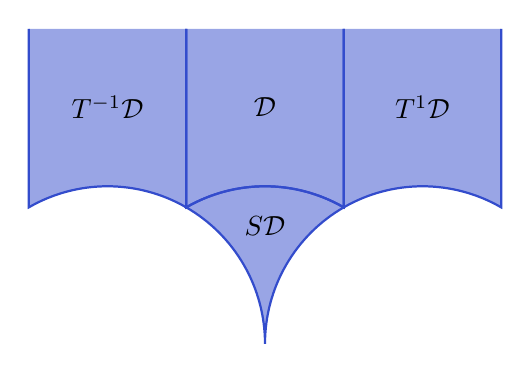
\begin{tikzpicture}

      \fill [opacity=0.5, mblue] (1, 4) -- (1, 1.732) arc (60:120:2) -- (-1, 4);
      \draw [mblue, thick] (1, 4) -- (1, 1.732) arc (60:120:2) -- (-1, 4);
      \node at (0, 3) {$\mathcal{D}$};

      \begin{scope}[shift={(2, 0)}]
        \fill [opacity=0.5, mblue] (1, 4) -- (1, 1.732) arc (60:120:2) -- (-1, 4);
        \draw [mblue, thick] (1, 4) -- (1, 1.732) arc (60:120:2) -- (-1, 4);
        \node at (0, 3) {$T^1\mathcal{D}$};
      \end{scope}
      \begin{scope}[shift={(-2, 0)}]
        \fill [opacity=0.5, mblue] (1, 4) -- (1, 1.732) arc (60:120:2) -- (-1, 4);
        \draw [mblue, thick] (1, 4) -- (1, 1.732) arc (60:120:2) -- (-1, 4);
        \node at (0, 3) {$T^{-1}\mathcal{D}$};
      \end{scope}

      \fill [opacity=0.5, mblue] (1, 1.732) arc(120:180:2) arc(0:60:2) arc(120:60:2);
      \draw [thick, mblue] (1, 1.732) arc(120:180:2) arc(0:60:2) arc(120:60:2);
      \node at (0, 1.5) {$S\mathcal{D}$};
    \end{tikzpicture}
  \end{center}
\end{eg}
So in defining modular forms, we'll want to control functions as $z \to 0$ (in some way), as well as when $y \to \infty$. In fact, what we really need is that the function has to be holomorphic at all points in $\P^1(\Q) = \Q \cup \{\infty\}$. It happens that in the case of $\Gamma(1)$, the group $\Gamma(1)$ acts transitively on $\Q \cup \{\infty\}$. So by invariance of $f$ under $\Gamma(1)$, being holomorphic at $\infty$ ensures we are holomorphic everywhere.

In general, we will have to figure out the orbits of $\Q \cup \{\infty\}$ under $\Gamma$, and then pick a representative of each orbit. Before we go into that, we first understand what the fundamental domain of $\Gamma$ looks like.

%Note that $\Gamma(1)$ acts transitively on $\P^1(\Q) = \Q \cup \{\infty\}$ by M\"obius transforms, but in general, subgroups $\Gamma$ don't. To see this, note that if $-\frac{d}{c} \in \Q$ and $(c, d) = 1$, Then there are $a, b \in \Z$ with $ad -b c = 1$ and $c, d \in \Z$. So we have
%\[
% \begin{pmatrix}
% a & b\\
% c & d
% \end{pmatrix}
% \frac{-d}{c} = \infty.
%\]
\begin{defi}[Cusps]\index{cusps}
  The \emph{cusps} of $\Gamma$ (or $\bar{\Gamma}$) are the orbits of $\Gamma$ on $\P^1(\Q)$.
\end{defi}
We would want to say a subgroup of index $n$ has $n$ many cusps, but this is obviously false, as we can see from our example above. The problem is that we should could each cusp with ``multiplicity''. We will call this the \emph{width}. For example, in the fundamental domain above
\begin{center}
  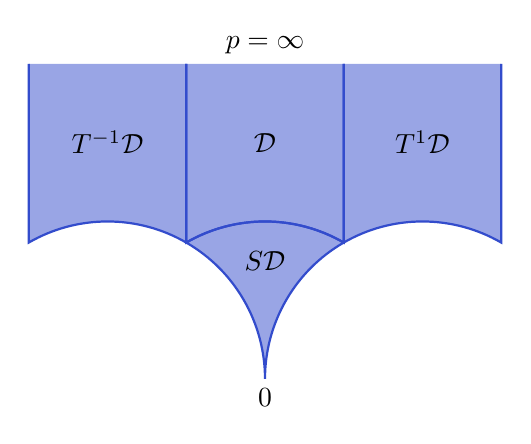
\begin{tikzpicture}

    \fill [opacity=0.5, mblue] (1, 4) -- (1, 1.732) arc (60:120:2) -- (-1, 4);
    \draw [mblue, thick] (1, 4) -- (1, 1.732) arc (60:120:2) -- (-1, 4);
    \node at (0, 3) {$\mathcal{D}$};

    \node [above] at (0, 4) {$p = \infty$};

    \begin{scope}[shift={(2, 0)}]
      \fill [opacity=0.5, mblue] (1, 4) -- (1, 1.732) arc (60:120:2) -- (-1, 4);
      \draw [mblue, thick] (1, 4) -- (1, 1.732) arc (60:120:2) -- (-1, 4);
      \node at (0, 3) {$T^1\mathcal{D}$};
    \end{scope}
    \begin{scope}[shift={(-2, 0)}]
      \fill [opacity=0.5, mblue] (1, 4) -- (1, 1.732) arc (60:120:2) -- (-1, 4);
      \draw [mblue, thick] (1, 4) -- (1, 1.732) arc (60:120:2) -- (-1, 4);
      \node at (0, 3) {$T^{-1}\mathcal{D}$};
    \end{scope}

    \fill [opacity=0.5, mblue] (1, 1.732) arc(120:180:2) arc(0:60:2) arc(120:60:2);
    \draw [thick, mblue] (1, 1.732) arc(120:180:2) arc(0:60:2) arc(120:60:2);
    \node at (0, 1.5) {$S\mathcal{D}$};

    \node [below] at (0, 0) {$0$};
  \end{tikzpicture}
\end{center}
In this case, we should count $p = \infty$ three times, and $p = 0$ once. One might worry this depends on which fundamental domain we pick for $\Gamma$. Thus, we will define it in a different way. From now on, it is more convenient to talk about $\bar{\Gamma}$ than $\Gamma$.

Since $\overline{\Gamma(1)}$ acts on $\P^1(\Q)$ transitively, it actually just suffices to understand how to define the multiplicity for the cusp of $\infty$. The stabilizer of $\infty$ in $\overline{\Gamma(1)}$ is
\[
  \overline{\Gamma(1)}_\infty = \left\{
  \pm \begin{pmatrix}
    1 & b\\
    0 & 1
  \end{pmatrix}: b \in \Z\right\}.
\]
For a general subgroup $\overline{\Gamma} \leq \overline{\Gamma(1)}$, the stabilizer of $\infty$ is $\overline{\Gamma}_\infty = \overline{\Gamma} \cap \overline{\Gamma(1)}_\infty$. Then this is a finite index subgroup of $\overline{\Gamma(1)}_\infty$, and hence must be of the form
\[
  \overline{\Gamma}_\infty = \left\bra \pm
  \begin{pmatrix}
    1 & m\\
    0 & 1
  \end{pmatrix}\right\ket
\]
for some $m \geq 1$. We define the width of the cusp to be this $m$.

More generally, for an arbitrary cusp, we define the width by conjugation.

\begin{defi}[Width of cusp]\index{width of cusp}
  Let $\alpha \in \Q \cup \{\infty\}$ be a representation of a cusp of $\Gamma$. We pick $g \in \Gamma(1)$ with $g(\infty) = \alpha$. Then $\gamma(\alpha) = \alpha$ iff $g^{-1}\gamma g(\infty) = \infty$. So
  \[
    g^{-1} \overline{\Gamma}_\alpha g = (\overline{g^{-1}\Gamma g})_\infty = \left\bra \pm
    \begin{pmatrix}
      1 & m_\alpha\\
      0 & 1
    \end{pmatrix}\right\ket
  \]
  for some $m_\alpha \geq 1$. This $m_\alpha$ is called the \emph{width} of the cusp $\alpha$ (i.e.\ the cusp $\Gamma \alpha$).
\end{defi}

The $g$ above is not necessarily unique. But if $g'$ is another, then
\[
  g' = g
  \begin{pmatrix}
    \pm 1 & n\\
    0 & \pm 1
  \end{pmatrix}
\]
for some $n \in \Z$. So $m_\alpha$ is independent of the choice of $g$.

As promised, we have the following proposition:
\begin{prop}
  Let $\Gamma$ have $\nu$ cusps of widths $m_1, \cdots, m_\nu$. Then
  \[
    \sum_{i = 1}^\nu m_i = (\overline{\Gamma(1)}: \bar{\Gamma}).
  \]
\end{prop}

\begin{proof}
  There is a surjective map
  \[
    \pi: \bar{\Gamma} \setminus \overline{\Gamma(1)} \to \text{cusps}
  \]
  given by sending
  \[
    \bar{\Gamma} \cdot \gamma \mapsto \bar{\Gamma}\cdot \gamma(\infty).
  \]
  It is then an easy group theory exercise that $|\pi^{-1}([\alpha])| = m_\alpha$.
%
% Let $\alpha = g(\infty) \in \P^1(\Q)$, and $g \in \Gamma(1)$. Then
% \begin{align*}
% \pi(\bar{\Gamma} \cdot \gamma g) = \bar{\Gamma} \cdot \alpha &\Longleftrightarrow\bar{\Gamma} \gamma g(\infty) = \bar{\Gamma} \alpha\\
% &\Longleftrightarrow \gamma(\alpha) \in \bar{\Gamma}_\alpha\\
% &\Longleftrightarrow \gamma \in \bar{\Gamma} \overline{\Gamma(1)}_\alpha.
% \end{align*}
% Now note that there is a bijection
% \[
% \frac{\bar{\Gamma} \cdot \overline{\Gamma(1)}_\alpha}{\bar{\Gamma}} \cong \frac{\bar{\Gamma(1)}_\alpha}{ \bar{\Gamma}_\alpha}
% \]
% by mapping $\bar{\Gamma} \gamma$ to $\bar{\Gamma}_\alpha \gamma$.
%
% So we know $\bar{\Gamma} \cdot \overline{\Gamma(1)}_\alpha$ is a disjoint union of $(\overline{\Gamma(1)}_\alpha: \bar{\Gamma}_\alpha) = m_\alpha$ cosets of $\bar{\Gamma}$. So $\pi^{-1}(\bar{\Gamma}_\alpha)$ has $m_\alpha$ elements.
\end{proof}

\begin{eg}
  Consider the following subgroup
  \[
    \Gamma = \Gamma_0(p) =\left\{
      \begin{pmatrix}
        a & b\\
        c & d
      \end{pmatrix} : c \equiv 0 \pmod p
    \right\}.
  \]
  Then we have
  \[
    \big(\overline{\Gamma(1)}: \overline{\Gamma_0(p)}\big) = \big(\Gamma(1): \Gamma_0(p)\big) = p + 1.
  \]
  We can compute
  \[
    \Gamma_\infty = \left\langle -1,
    \begin{pmatrix}
      1 & 1\\
      0 & 1
    \end{pmatrix}\right\rangle = \Gamma(1)_\infty.
  \]
  So $m_\infty = 1$. But we also have
  \[
    \Gamma_0 = \left\langle -1,
    \begin{pmatrix}
      1 & 0\\
      p & 1
    \end{pmatrix}\right\rangle,
  \]
  and this gives $m_0 = p$. Since $p + 1 = p = 1$, these are the only cusps of $\Gamma_0(p)$. Likewise, for $\Gamma^0(p)$, we have $m_\infty = p$ and $m_0 = 1$.
%
% Geometrically, the width of a cusp $\alpha$ is the number of copies of fundamental domain where the boundary meets $\alpha$:
% \begin{center}
% \begin{tikzpicture}
%
% \fill [opacity=0.5, mblue] (1, 4) -- (1, 1.732) arc (60:120:2) -- (-1, 4);
% \draw [mblue, thick] (1, 4) -- (1, 1.732) arc (60:120:2) -- (-1, 4);
% \node at (0, 3) {$\mathcal{D}$};
%
% \node [above] at (0, 4) {$p = \infty$};
%
% \begin{scope}[shift={(2, 0)}]
% \fill [opacity=0.5, mblue] (1, 4) -- (1, 1.732) arc (60:120:2) -- (-1, 4);
% \draw [mblue, thick] (1, 4) -- (1, 1.732) arc (60:120:2) -- (-1, 4);
% \node at (0, 3) {$T^1\mathcal{D}$};
% \end{scope}
% \begin{scope}[shift={(-2, 0)}]
% \fill [opacity=0.5, mblue] (1, 4) -- (1, 1.732) arc (60:120:2) -- (-1, 4);
% \draw [mblue, thick] (1, 4) -- (1, 1.732) arc (60:120:2) -- (-1, 4);
% \node at (0, 3) {$T^{-1}\mathcal{D}$};
% \end{scope}
%
% \fill [opacity=0.5, mblue] (1, 1.732) arc(120:180:2) arc(0:60:2) arc(120:60:2);
% \draw [thick, mblue] (1, 1.732) arc(120:180:2) arc(0:60:2) arc(120:60:2);
% \node at (0, 1.5) {$S\mathcal{D}$};
%
% \node [below] at (0, 0) {$0$};
% \end{tikzpicture}
% \end{center}
\end{eg}

Equipped with the definition of a cusp, we can now define a modular form!
\begin{defi}[Modular form]\index{modular form}
  Let $\Gamma \subseteq \SL_2(\Z)$ be of finite index, and $k \in \Z$. A \emph{modular form of weight $k$ on $\Gamma$} is a holomorphic function $f: \H \to \C$ such that
  \begin{enumerate}
    \item $f\underset{k}{|} \gamma = f$ for all $\gamma \in \Gamma$.
    \item $f$ is holomorphic at the cusps of $\Gamma$.
  \end{enumerate}
  If moreover,
  \begin{enumerate}
    \item[(iii)] $f$ vanishes at the cusps of $\Gamma$,
  \end{enumerate}
  then we say $f$ is a \term{cusp form}.
\end{defi}
As before, we have to elaborate a bit more on what we mean by (ii) and (iii). We already know what it means when the cusp is $\infty$ (i.e.\ it is $\Gamma \infty$). Now in general, we write our cusp as $\Gamma \alpha = \Gamma g(\infty)$ for some $g \in \Gamma(1)$.

Then we know
\[
  \bar{\Gamma}_\alpha = g \left\bra \pm
  \begin{pmatrix}
    1 & m\\
    0 & 1
  \end{pmatrix}\right\ket g^{-1}.
\]
This implies we must have
\[
  \begin{pmatrix}
    1 & m\\
    0 & 1
  \end{pmatrix}\text{ or }-
  \begin{pmatrix}
    1 & m\\
    0 & 1
  \end{pmatrix} \in g^{-1}\Gamma_\alpha g.
\]
Squaring, we know that we must have
\[
  \begin{pmatrix}
    1 & 2m\\
    0 & 1
  \end{pmatrix} \in g^{-1} \Gamma_\alpha g.
\]
So we have
\[
  f \underset{k}{|} g \underset{k}{|}
  \begin{psmallmatrix}
    1 & 2m\\
    0 & 1
  \end{psmallmatrix} = f \underset{k}{|} g.
\]
So we know
\[
  (f\underset{k}{|}g) (z + 2m) = (f\underset{k}{|}g)(z).
\]
Thus, we can write
\[
  f\underset{k}{|} g = \tilde{f}_g(q) = \sum_{n \in \Z} (\text{constant}) q^{n/2m} = \sum_{\substack{n \in \Q\\ 2mn \in \Z}} a_{g, n}(f) q^n,
\]
where we define
\[
  q^{a/b} = e^{2\pi i a z/b}.
\]
Then $f$ is holomorphic at the cusp $\alpha = g(\infty)$ if
\[
  a_{g, n}(f) = 0
\]
for all $n < 0$, and \emph{vanishes} at $\alpha$ if moreover
\[
  a_{g, 0}(f) = 0.
\]
Note that if $-I \in \Gamma$, then in fact
\[
  \begin{pmatrix}
    1 & m\\
    0 & 1
  \end{pmatrix} \in g^{-1} \Gamma_\alpha g.
\]
So the ``$q$ expansion at $\alpha$'' is actually series in $q^{1/m}$.

\separator

There is a better way of phrasing this. Suppose we have $g(\infty) = \alpha = g'(\infty)$, where $g' \in \GL_2(\Q)^+$. Then we have
\[
  g' = gh
\]
for some $h \in \GL_2(\Q)^+$ such that $h(\infty) = \infty$. So we can write
\[
  h = \pm
  \begin{pmatrix}
    a & b\\
    0 & c
  \end{pmatrix}
\]
where $a, b, d \in \Q$ and $a, d > 0$.

Then, we have
\begin{align*}
  f\underset{k}{|} g' &= (f \underset{k}{|} g) \underset{k}{|} h \\
  &= \sum_{\substack{n \in \Q \\ 2mn \in \Z}} a_{g, n} (f) q^n \underset{k}{|} \pm
  \begin{psmallmatrix}
    a & b\\
    0 & d
  \end{psmallmatrix}\\
  &= (\pm i)^k \sum_n a_{g, n} (f) q^{an/d} e^{2\pi bn/d}.
\end{align*}
In other words, we have
\[
  f\underset{k}{|} g = \sum_{n \geq 0} c_n q^{rn}
\]
for some positive $r \in \Q$. So condition (ii) is equivalent to (ii'):
\begin{enumerate}
  \item[(ii')] For all $g \in \GL_2(\Q)^+$, the function $f\underset{k}{|} g$ is holomorphic at $\infty$.
\end{enumerate}

Note that (ii') doesn't involve $\Gamma$, which is convenient. Likewise, (iii) is consider to
\begin{enumerate}
  \item[(iii')] $f\underset{k}{|} g$ vanishes at $\infty$ for all $g \in \GL_2(\Q)^+$.
\end{enumerate}
We can equivalently replace $\GL_2(\Q)^+$ with $\SL_2(\Z)$.

Modular form and cusp forms of weight $k$ on $\Gamma$ form a vector space $M_k(\Gamma) \supseteq S_k(\Gamma)$.

Recall that for $\Gamma = \Gamma(1) = \SL_2(\Z)$, we knew $M_k = 0$ if $k$ is odd, because
\[
  f\underset{k}{|} (-I) = (-1)^k f.
\]
More generally, if $-I \in \Gamma$, then $M_k = 0$ for all odd $k$. But if $-I \not\in \Gamma$, then usually there can be non-zero forms of odd weight.

Let's see some examples of such things.

\begin{prop}
  Let $\Gamma \subseteq \Gamma(1)$ be of finite index, and $g \in G = \GL_2(\Q)^+$. Then $\Gamma' = g^{-1} \Gamma g \cap \Gamma(1)$ also has finite index in $\Gamma(1)$, and if $f \in M_k(\Gamma)$ or $S_k(\Gamma)$, then $f\underset{k}{|} g \in M_k(\Gamma')$ or $S_k(\Gamma')$ respectively.
\end{prop}

\begin{proof}
  We saw that $(G, \Gamma)$ has property (H). So this implies the first part. Now if $\gamma \in \Gamma'$, then $g\gamma g^{-1} \in \Gamma$. So
  \[
    f \underset{k}{|}g \gamma g^{-1} = f \Rightarrow f\underset{k}{|} g \underset{k}{|}\gamma = f\underset{k}{|} g.
  \]
  The conditions (ii') and (iii') are clear.
\end{proof}
This provides a way of producing a lot of modular forms. For example, we can take $\Gamma = \Gamma(1)$, and take
\[
  g =
  \begin{pmatrix}
    N & 0\\
    0 & 1
  \end{pmatrix}.
\]
Then it is easy to see that $\Gamma' = \Gamma_0(N)$. So if $f(z) \in M_k(\Gamma(1))$, then $f(Nz) \in M_k(\Gamma_0(N))$. But in general, there are lots of modular forms in $\Gamma_0(N)$ that cannot be constructed this way.

As before, we don't have a lot of modular forms in low dimensions, and there is also an easy bound for those in higher dimensions.
\begin{thm}
  We have
  \[
    M_k(\Gamma) =
    \begin{cases}
      0 & k < 0\\
      \C & k = 0
    \end{cases},
  \]
  and
  \[
    \dim_\C M_k(\Gamma) \leq 1 + \frac{k}{12} (\Gamma(1): \Gamma).
  \]
  for all $k > 0$.
\end{thm}
In contrast to the case of modular forms of weight $1$, we don't have explicit generators for this.

\begin{proof}
  Let
  \[
    \Gamma(1) = \coprod_{i = 1}^d \Gamma \gamma_i.
  \]
  We let
  \[
    f \in M_k(\Gamma),
  \]
  and define
  \[
    \mathcal{N}_f = \prod_{1 \leq i \leq d} f\underset{k}{|} \gamma_i.
  \]
  We claim that $\mathcal{N}_f \in M_{kd} (\Gamma(1))$, and $\mathcal{N}_f = 0$ iff $f = 0$. The latter is obvious by the principle of isolated zeroes.

  Indeed, $f$ is certainly holomorphic on $\H$, and if $\gamma \in \Gamma(1)$, then
  \[
    \mathcal{N}_f\underset{k}{|} \gamma = \prod_i f\underset{k}{|} \gamma_i \gamma = \mathcal{N}_f.
  \]
  As $f \in M_k(\Gamma)$, each $f\underset{k}{|} \gamma_i$ is holomorphic at $\infty$.
  \begin{itemize}
    \item If $k < 0$, then $\mathcal{N}_f \in M_{kd} (\Gamma(1)) = 0$. So $f = 0$.
    \item If $k \geq 0$, then suppose $\dim M_k(G) > N$. Pick $z_1, \cdots, z_N \in \mathcal{D} \setminus \{i, \rho\}$ distinct. Then there exists $0 \not= f \in M_k(\Gamma)$ with
      \[
        f(z_1) = \cdots = f(z_N) = 0.
      \]
      So
      \[
        \mathcal{N}_f(z_1) = \cdots = \mathcal{N}_f (z_N) = 0.
      \]
      Then by our previous formula for zeros of modular forms, we know $N \leq \frac{kd}{12}$. So $\dim M_k(\Gamma) \leq1 + \frac{kd}{12}$.
    \item If $k = 0$, then $M_0(\Gamma)$ has dimension $\leq 1$. So $M_0(\Gamma) = \C$.
  \end{itemize}
\end{proof}

\subsection{The Petersson inner product}
As promised earlier, we define an inner product on the space of cusp forms.

We let $f, g \in S_k(\Gamma)$. Then the function $y^k f(z) \overline{g(z)}$ is $\Gamma$-invariant, and is bounded on $\H$, since $f$ and $g$ vanish at cusps. Also, recall that $\frac{\d x\; \d y}{y^2}$ is an $\GL_2(\R)^+$-invariant measure. So we can define
\[
  \bra f, g\ket = \frac{1}{v(\Gamma)} \int_{\Gamma \setminus \H} y^k f(z) \overline{g(z)} \frac{\d x\; \d y}{y^z} \in \C,
\]
where $\int_{\Gamma \setminus \H}$ means we integrate over any fundamental domain, and $v(\Gamma)$ is the volume of a fundamental domain,
\[
  v(\Gamma) = \int_{\Gamma \H} \frac{\d x\; \d y}{y^2} = (\overline{\Gamma(1)}:\bar{\Gamma}) \int_\mathcal{D} \frac{\d x\;\d y}{y^2}.
\]
The advantage of this normalization is that if we replace $\Gamma$ by a subgroup $\Gamma'$ of finite index, then a fundamental domain for $\Gamma'$ is the union of $(\bar{\Gamma}: \bar{\Gamma}')$ many fundamental domains for $\Gamma$. So the expression $(*)$ is \emph{independent} of $\Gamma$, as long as both $f, g \in S_k(\Gamma)$.

This is called the \term{Petersson inner product}.

\begin{prop}\leavevmode
  \begin{enumerate}
    \item $\bra\ph, \ph\ket$ is a Hermitian inner product on $S_k(\Gamma)$.
    \item $\bra \ph, \ph\ket$ is invariant under translations by $\GL_2(\Q)^+$. In other words, if $\gamma \in \GL_2(\Q)^+$, then
      \[
        \bra f\underset{k}{|}\gamma, g \underset{k}{|} \gamma\ket = \bra f, g\ket.
      \]
    \item If $f, g \in S_k(\Gamma(1))$, then
      \[
        \bra T_n f, g\ket = \bra f, T_n g\ket.
      \]
  \end{enumerate}
\end{prop}
This completes our previous proof that the $T_n$ can be simultaneously diagonalized.

\begin{proof}\leavevmode
  \begin{enumerate}
    \item We know $\bra f, g\ket$ is $\C$-linear in $f$, and $\overline{\bra f, g\ket} = \bra g, f\ket$. Also, if $\bra f, f \ket = 0$, then
      \[
        \int_{\Gamma \setminus \H} y^{k - 2} |f|^2 \;\d x \;\d y = 0,
      \]
      but since $f$ is continuous, and $y$ is never zero, this is true iff $f$ is identically zero.
    \item Let $f' = f\underset{k}{|} \gamma$ and $g' = g \underset{k}{|}\gamma \in S_k(\Gamma')$, where $\Gamma' = \Gamma \cap \gamma^{-1} \Gamma \gamma$. Then
      \[
        y^k f' \bar{g}' = y^k \frac{(\det \gamma)^k}{|cz + d|^{2k}} \cdot f(\gamma(z)) \overline{g(\gamma(z))} = (\Im \gamma(z))^k f(\gamma(z)) \overline{g(\gamma(z))}.
      \]
      Now $\Im \gamma(z)$ is just the $y$ of $\gamma(z)$. So it follows that
      Then we have
      \begin{align*}
        \bra f', g'\ket &= \frac{1}{v(\Gamma')} \int_{\mathcal{D}_{\Gamma'}} \left.y^k f \bar{g} \frac{\d x\;\d y}{y^2}\right|_{\gamma(z)} \\
        &= \frac{1}{v(\Gamma')} \int_{\gamma(\mathcal{D}_{\Gamma'})} y^k f \bar{g} \frac{\d x\;\d y}{y^2}.
      \end{align*}
      Now $\gamma(\mathcal{D}_{\Gamma'})$ is a fundamental domain for $\gamma \Gamma'\gamma^{-1} = \gamma \Gamma \gamma^{-1} \Gamma$, and note that $v(\Gamma') = v(\gamma \Gamma' \gamma^{-1})$ by invariance of measure. So $\bra f', g'\ket = \bra f, g\ket$.
    \item Note that $T_n$ is a polynomial with integer coefficients in $\{T_p : p \mid n\}$. So it is enough to do it for $n = p$. We claim that
      \[
        \bra T_p f, g\ket = p^{\frac{k}{2} - 1} (p + 1) \bra f\underset{k}{|} \delta, g\ket,
      \]
      where $\delta \in \Mat_2(\Z)$ is any matrix with $\det (\delta) = p$.

      Assuming this, we let
      \[
        \delta^a = p \delta^{-1} \in \Mat_2(\Z),
      \]
      which also has determinant $p$. Now as
      \[
        g \underset{k}{|}
        \begin{psmallmatrix}
          p & 0\\
          0 & p
        \end{psmallmatrix} = g,
      \]
      we know
      \begin{align*}
        \bra T_p f, g\ket &= p^{\frac{k}{2} - 1}(p + 1) \bra f\underset{k}{|}\delta, g\ket \\
        &= p^{\frac{k}{2} - 1} (p + 1) \bra f, g \underset{k}{|} \delta^{-1}\ket \\
        &= p^{\frac{k}{2} - 1} (p + 1) \bra f, g \underset{k}{|} \delta^{a }\ket \\
        &= \bra f, T_p g\ket
      \end{align*}
      To prove the claim, we let
      \[
        \Gamma(1)
        \begin{pmatrix}
          p & 0\\
          0 & 1
        \end{pmatrix} \Gamma(1) =
        \coprod_{0 \leq j \leq p} \Gamma(1) \delta \gamma_i
      \]
      for some $\gamma_i \in \Gamma(1)$. Then we have
      \begin{align*}
        \bra T_p f, g\ket &= p^{\frac{k}{2} - 1} \left\bra \sum_j f \underset{k}{|} \delta \gamma_j, g\right\ket\\
        &= p^{\frac{k}{2} - 1} \sum_j \bra f\underset{k}{|} \delta \gamma_j, g \underset{k}{|} \gamma_j\ket \\
        &= p^{\frac{k}{2} - 1} (p + 1) \bra f\underset{k}{|} \delta, g\ket,
      \end{align*}
      using the fact that $g \underset{k}{|} \gamma_j = g$.
  \end{enumerate}
\end{proof}

\subsection{Examples of modular forms}
We now look at some examples of (non-trivial) modular forms for different subgroups. And the end we will completely characterize $M_2(\Gamma_0(4))$. This seems like a rather peculiar thing to completely characterize, but it turns out this understanding $M_2(\Gamma_0(4))$ can allow us to prove a rather remarkable result!

\subsubsection*{Eisenstein series}
At the beginning of the course, the first example of a modular form we had was Eisenstein series. It turns out a generalized version of Eisenstein series will give us more modular forms.

\begin{defi}[$G_{\mathbf{r}, k}$]\index{$G_{\mathbf{r}, k}$}
  Let $k \geq 3$. Pick any vector $\mathbf{r} = (r_1, r_2) \in \Q^2$. We define
  \[
    G_{\mathbf{r}, k}(z) = \sideset{}{'}\sum_{\mathbf{m} \in \Z^2} \frac{1}{((m_1 + r_1) z + m_2 + r_2)^k},
  \]
  where $\sum'$ means we omit any $\mathbf{m}$ such that $\mathbf{m} + \mathbf{r} = \mathbf{0}$.
\end{defi}
For future purposes, we will consider $\mathbf{r}$ as a row vector.

As before, we can check that this converges absolutely for $k \geq 3$ and $z \in \H$. This obviously depends only on $\mathbf{r} \bmod \Z^2$, and
\[
  G_{\mathbf{0}, k} = G_k.
\]

\begin{thm}\leavevmode
  \begin{enumerate}
    \item If $\gamma \in \Gamma(1)$, then
      \[
        G_{\mathbf{r}, k}\underset{k}{|}\gamma = G_{\mathbf{r} \gamma, k}.
      \]
    \item If $N\mathbf{r} \in \Z^2$, then $G_{\mathbf{r}, k} \in M_k(\Gamma(N))$.
  \end{enumerate}
\end{thm}

\begin{proof}\leavevmode
  \begin{enumerate}
    \item If $g \in \GL_2(\R)^+$ and $\mathbf{u} \in \R^2$, then
      \[
        \frac{1}{(u_1 z + u_2)^k} \underset{k}{|} g = \frac{(\det g)^{k/2}}{ ((au_1 + cu_2) z + (bu_1 + d u_2))^k} = \frac{(\det g)^{k/2}}{(v_1 z + v_2)^k},
      \]
      where $\mathbf{v} = \mathbf{n}\cdot g$. So
      \begin{align*}
        G_{\mathbf{r}, k} \underset{k}{|}\gamma &= \sideset{}{'}\sum_{\mathbf{m}}\frac{1}{(((\mathbf{m} + \mathbf{r})_1 \gamma) z + ((\mathbf{m} + \mathbf{r})\gamma)_2)^k} \\
        &= \sum_{\mathbf{m}'} \frac{1}{((m_1' + r_1') z + m_2' + r_2')^k}\\
        &= G_{\mathbf{r} \gamma, k}(z),
      \end{align*}
      where $\mathbf{m}' = \mathbf{m} \gamma$ and $\mathbf{r}' = \mathbf{r} \gamma$.
    \item By absolute convergence, $G_{\mathbf{r}, k}$ is holomorphic on the upper half plane. Now if $N\mathbf{r} \in \Z^2$ and $\gamma \in \Gamma(N)$, then $N\mathbf{r} \gamma \equiv N\mathbf{r} \pmod N$. So $\mathbf{r} \gamma \equiv \mathbf{r} \pmod {\Z^2}$. So we have
      \[
        G_{\mathbf{r}, k}\underset{k}{|}\gamma = G_{\mathbf{r} \gamma, k} = G_{\mathbf{r}, k}.
      \]
      So we get invariance under $\Gamma(N)$. So it is enough to prove $G_{\mathbf{r}, k}$ is holomorphic at cusps, i.e.\ $G_{\mathbf{r}, k}\underset{k}{|} \gamma$ is holomorphic at $\infty$ for all $\gamma \in \Gamma(1)$. So it is enough to prove that for \emph{all} $\mathbf{r}$, $G_{\mathbf{r}, k}$ is holomorphic at $\infty$.

      We can write
      \[
        G_{\mathbf{r}, k} = \left(\sum_{m_1 + r_1 > 0} + \sum_{m_1 + r_1 = 0} + \sum_{m_1 + r_1 < 0}\right)\frac{1}{((m_1 + r_1) z + m_2 + r_2)^k}.
      \]
      The first sum is
      \[
        \sum_{m_1 + r_1 > 0} = \sum_{m_1 > - r_1} \sum_{m_2 \in \Z} \frac{1}{([(m_1 + r_1) z + r_2] + m_2)^k}.
      \]
      We know that $(m_1 + r_1)z + r_2 \in \H$. So we can write this as a Fourier series
      \[
        \sum_{m_1 > -r_1} \sum_{d \geq 1} \frac{(-2\pi)^k}{(k - 1)!} d^{k - 1} e^{2\pi r_2 d} q^{(m_1 + r_1) d}.
      \]
      We now see that all powers of $q$ are positive. So this is holomorphic.

      The sum over $m_1 + r_1 = 0$ is just a constant. So it is fine.

      For the last term, we have
      \[
        \sum_{m_1 + r_1 < 0} = \sum_{m_1 < - r_1} \sum_{m_2 \in \Z} \frac{(-1)^k}{((-m_1 - r_1)z - r_2 - m_2)^k},
      \]
      which is again a series in positive powers of $q^{-m_1 - r_1}$.
  \end{enumerate}
\end{proof}

\subsubsection*{\tph{$\vartheta$}{theta}{&theta;} functions}
Our next example of modular forms is going to come from $\vartheta$ functions. We previously defined a $\vartheta$ function, and now we are going to call it $\vartheta_3$:\index{$\vartheta_3$}
\[
  \vartheta_3(z) = \vartheta(z) = \sum_{n \in \Z} e^{\pi in^2 z} = 1 + 2 \sum_{n \geq 1} q^{n^2/2}.
\]
We proved a functional equation for this, which was rather useful.

Unfortunately, this is not a modular form. Applying elements of $\Gamma(1)$ to $\vartheta_3$ will give us some new functions, which we shall call $\vartheta_2$ and $\vartheta_4$.

\begin{defi}[$\vartheta_2$ and $\vartheta_4$]\index{$\vartheta_2$}\index{$\vartheta_4$}
  \begin{align*}
    \vartheta_2(z) &= \sum_{n \in \Z} e^{\pi i (n + 1/2)^2 z} = q^{1/8} \sum_{n \in \Z} q^{n(n + 1)/2} = 2 q^{1/8} \sum_{n \geq 0} q^{n(n + 1)/2}\\
    \vartheta_4(z) &= \sum_{n \in \Z} (-1)^n e^{\pi i n^2 z} = 1 + 2 \sum_{n \geq 1} (-1)^n q^{n^2/2}.
  \end{align*}
\end{defi}

\begin{thm}\leavevmode
  \begin{enumerate}
    \item $\vartheta_4(z) = \vartheta_3(z \pm 1)$ and $\theta_2(z + 1) = e^{\pi i/4} \vartheta_2(z)$.
    \item
      \begin{align*}
        \vartheta_3\left(-\frac{1}{z}\right) &= \left(\frac{z}{i}\right)^{1/2} \vartheta_3(z)\\
        \vartheta_4 \left(-\frac{1}{z}\right) &= \left(\frac{z}{i}\right)^{1/2} \vartheta_2(z)
      \end{align*}
  \end{enumerate}
\end{thm}

\begin{proof}\leavevmode
  \begin{enumerate}
    \item Immediate from definition, e.g.\ from the fact that $e^{\pi i} = 1$.
    \item The first part we've seen already. To do the last part, we use the Poisson summation formula. Let
      \[
        h_t(x) = e^{-\pi t(x + 1/2)^2} = g_t\left(x + \frac{1}{2}\right),
      \]
      where
      \[
        g_t(x) = e^{-\pi tx^2}.
      \]
      We previously saw
      \[
        \hat{g}_t(y) = t^{-1/2} e^{-\pi y^2/t}.
      \]
      We also have
      \begin{align*}
        \hat{h}_t(y) &= \int e^{-2\pi i xy} g_t\left(x + \frac{1}{2}\right)\;\d x \\
        &= \int e^{-2\pi i (x - 1/2) y} g_t(x) \;\d x \\
        &= e^{\pi i y} \hat{g}_t(y).
      \end{align*}
      So by the Poisson summation formula,
      \[
        \vartheta_2(it) = \sum_{n \in \Z} h_t(n) = \sum_{n \in \Z} \hat{h}_t(n) = \sum_{n \in \Z} (-1)^n t^{-1/2} e^{-\pi n^2/t} = t^{-1/2} \vartheta_4 \left(\frac{i}{t}\right).
      \]
  \end{enumerate}
\end{proof}
There is also a $\vartheta_1$, but we have $\vartheta_1 = 0$. Of course, we did not just invent a funny name for the zero function for no purpose. In general, we can define functions $\vartheta_j(u, z)$, and the $\vartheta$ functions we defined are what we get when we set $u = 0$. It happens that $\vartheta_1$ has the property that
\[
  \vartheta_1(u, z) = - \vartheta_1(-u, z),
\]
which implies $\vartheta_1(z) = 0$.

We now see that the action of $\SL_2(\Z)$ send us between $\vartheta_2$, $\vartheta_3$ and $\vartheta_4$, up to simple factors.

\begin{cor}\leavevmode
  \begin{enumerate}
    \item Let
      \[
        F =
        \begin{pmatrix}
          \vartheta_2^4\\
          \vartheta_3^4\\
          \vartheta_4^4
        \end{pmatrix}.
      \]
      Then
      \[
        F(z + 1) =
        \begin{pmatrix}
           -1 & 0 & 0\\
           0 & 0 & 1\\
           0 & 1 & 0
         \end{pmatrix} F,\quad z^{-2} F\left(-\frac{1}{z}\right) =
         \begin{pmatrix}
           0 & 0 & -1\\
           0 & -1 & 0\\
           -1 & 0 & 0
         \end{pmatrix}F
      \]
    \item $\vartheta_j^4 \in M_2(\Gamma)$ for a subgroup $\Gamma \leq \Gamma(1)$ of finite index. In particular, $\vartheta_j^4 \underset{z}{|} \gamma$ is holomorphic at $\infty$ for any $\gamma \in \GL_2(\Q)^+$.
  \end{enumerate}
\end{cor}
\begin{proof}\leavevmode
  \begin{enumerate}
    \item Immediate from the theorem.
    \item We know $\overline{\Gamma(1)} = \bra S, T\ket$, where $T = \pm \begin{psmallmatrix}1 & 1\\0 & 1\end{psmallmatrix}$ and $S = \pm \begin{psmallmatrix}0 & -1\\1 & 0\end{psmallmatrix}$. So by (i), there is a homomorphism $\rho: \Gamma(1) \to \GL_3(\Z)$ and $\rho(-I) = I$ with
      \[
        F\underset{2}{|} \gamma = \rho(\gamma) F,
      \]
      where $\rho(\gamma)$ is a signed permutation. In particular, the image of $\rho$ is finite, so the kernel $\Gamma = \ker \rho$ has finite index, and this is the $\Gamma$ we want.

      It remains to check holomorphicity. But each $\vartheta_j$ is holomorphic at $\infty$. Since $F\underset{2}{|} \gamma= \rho (\gamma) F$, we know $\vartheta_j^4\underset{2}{|}$ is a sum of things holomorphic at $\infty$, and is hence holomorphic at $\infty$.
  \end{enumerate}
\end{proof}

It would be nice to be more specific about exactly what subgroup $\vartheta_j^4$ is invariant under. Of course, whenever $\gamma \in \Gamma$, then we have $\vartheta_j^4 \underset{2}{|}\gamma = \vartheta_j^4$. But in fact $\vartheta_j^4$ is invariant under a larger group.

To do this, it suffices to do it for $\vartheta^4 = \vartheta_3^4$, and the remaining follow by conjugation.

We introduce a bit of notation
\begin{notation}
  We write\index{$W_N$}
  \[
    W_N =
    \begin{pmatrix}
      0 & -1\\
      N & 0
    \end{pmatrix}
  \]
\end{notation}
Note that in general, $W_N$ does \emph{not} have determinant $1$.

\begin{thm}
  Let $f(z) = \vartheta(2z)^4$. Then $f(z) \in M_2(\Gamma_0(4))$, and moreover, $f\underset{2}{|}W_4 = -f$.
\end{thm}

To prove this, we first note the following lemma:
\begin{lemma}
  $\Gamma_0(4)$ is generated by
  \[
    -I,\quad
    T=
    \begin{pmatrix}
      1 & 1\\0 & 1
    \end{pmatrix},
    \quad
    U=
    \begin{pmatrix}
      1 & 0\\
      4 & 1
    \end{pmatrix} =
    W_4
    \begin{pmatrix}
      1 & -1 \\
      0 & 1
    \end{pmatrix}
    W_4^{-1}.
  \]
\end{lemma}
Four is special. This is not a general phenomenon.

\begin{proof}
  It suffices to prove that $\overline{\Gamma_0(4)}$ is generated by $T$ and $U = \pm \begin{psmallmatrix} 1 & 0\\ 4 & 1 \end{psmallmatrix}$.

  Let
  \[
    \gamma = \pm
    \begin{pmatrix}
      a & b\\
      c & d
    \end{pmatrix} \in \overline{\Gamma_0(4)}.
  \]
  We let
  \[
    s(\gamma) = a^2 + b^2.
  \]
  As $c$ is even, we know $a \equiv 1 \pmod 2$. So $s(\gamma) \geq 1$, and moreover $s(\gamma) = 1$ iff $b = 0, a = \pm 1$, iff $\gamma = T^n$ for some $n$.

  We now claim that if $s(\gamma) \not= 1$, then there exists $\delta \in \{T^{\pm 1}, U^{\pm 1}\}$ such that $s(\gamma\delta) < s(\gamma)$. If this is true, then we are immediately done.

  To prove the claim, if $s(\gamma) \not= 1$, then note that $|a| \not= |2b|$ as $a$ is odd.
  \begin{itemize}
    \item If $|a| < |2b|$, then $\min\{|b \pm a|\} < |b|$. This means $s(\gamma T^{\pm 1}) = a^2 + (b \pm a)^2 < s(\gamma)$.
    \item If $|a| > |2b|$, then $\min \{|a \pm 4b|\} < |a|$, so $s(\gamma U^{\pm 1}) = (a \pm 4b)^2 + b^2 < s(\gamma)$.
  \end{itemize}
\end{proof}

\begin{proof}[Proof of theorem]
  It is enough to prove that
  \[
    f\underset{2}{|}T = f\underset{2}{|} U = f.
  \]
  This is now easy to prove, as it is just a computation. Since $\vartheta(z + 2) = \vartheta(z)$, we know
  \[
    f\underset{2}{|} T = f(z + 1) = f(z).
  \]
  We also know that
  \[
    f\underset{2}{|} W_4 = 4 (4z)^{-2} f\left(\frac{-1}{4z}\right) = \frac{1}{4 z^2} \vartheta\left(-\frac{1}{2z}\right)^4 = - f(z),
  \]
  as
  \[
    \vartheta\left(-\frac{1}{z}\right) = \left(\frac{z}{i}\right)^{1/2} \vartheta(z).
  \]
  So we have
  \[
    f\underset{2}{|} U = f\underset{2}{|} W_4 \underset{2}{|} T^{-1} \underset{2}{|} W_4 = (-1)(-1)f = f.
  \]
\end{proof}

We look at $\Gamma_0(2)$ and $\Gamma_0(4)$ more closely. We have
\[
  \Gamma_0(2) = \left\{
    \begin{pmatrix}
      a & b\\
      2c & d
    \end{pmatrix}
  \right\} = \left\{\gamma \in \Gamma(1): \gamma =
    \begin{pmatrix}
      1 & *\\
      0 & 1
    \end{pmatrix}\mod 2
  \right\}.
\]
We know $|\SL_2(\Z/2\Z)| = 6$, and so $(\Gamma(1): \Gamma_0(2)) = 3$. We have coset representatives
\[
  I,
  \begin{pmatrix}
    0 & -1\\
    0 & 1
  \end{pmatrix},
  \begin{pmatrix}
    1 & 0\\
    1 & 1
  \end{pmatrix}.
\]
We also have a map
\begin{align*}
  \Gamma_0(2) &\twoheadrightarrow \Z/2\Z\\
  \begin{pmatrix}
    a & b\\
    2c & d
  \end{pmatrix} &\mapsto c,
\end{align*}
which one can directly check to be a homomorphism. This has kernel $\Gamma_0(4)$. So we know $(\Gamma_0(2) : \Gamma_0(4)) = 2$, and has coset representatives
\[
  I,
  \begin{pmatrix}
    1 & 0\\
    2 & 1
  \end{pmatrix}
\]
So
\[
  \overline{\Gamma_0(2)} = \left\bra T,
  \pm
  \begin{pmatrix}
    1 & 0\\
    2 & 1
  \end{pmatrix} = W_2
  \begin{pmatrix}
    1 & 1\\
    0 & 1
  \end{pmatrix} W_2^{-1}\right\ket.
\]
We can draw fundamental domains for $\Gamma^0(2)$:
\begin{center}
  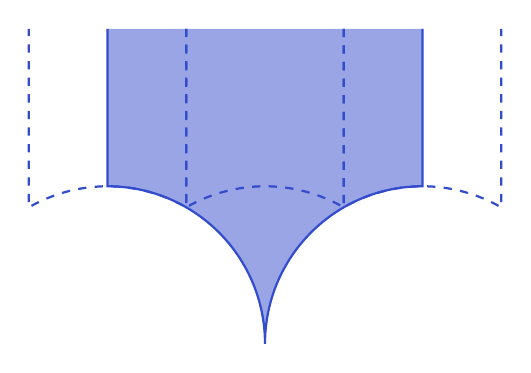
\begin{tikzpicture}
    \draw [mblue, thick, dashed] (1, 4) -- (1, 1.732) arc (60:120:2) -- (-1, 4);

    \begin{scope}[shift={(2, 0)}, xscale=-1]
      \draw [mblue, thick, dashed] (1, 4) -- (1, 1.732) arc (60:120:2) -- (-1, 4);
    \end{scope}

    \begin{scope}[shift={(-2, 0)}]
      \draw [mblue, thick, dashed] (1, 4) -- (1, 1.732) arc (60:120:2) -- (-1, 4);
    \end{scope}

    \fill [opacity=0.5, mblue] (2, 4) -- (2, 2) arc(90:180:2) arc(0:90:2) -- (-2, 4);
    \draw [thick, mblue] (2, 4) -- (2, 2) arc(90:180:2) arc(0:90:2) -- (-2, 4);
  \end{tikzpicture}
\end{center}
and $\Gamma^0(4)$:
\begin{center}
  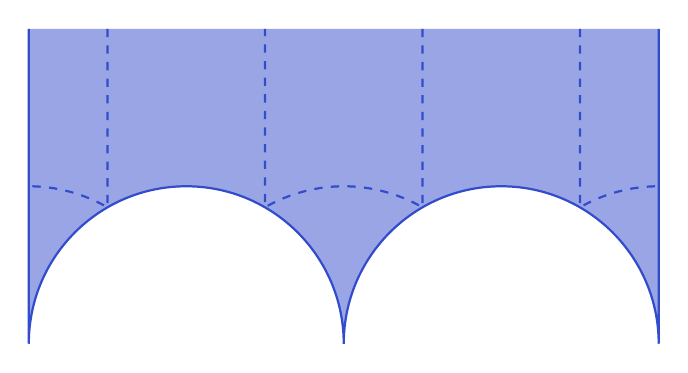
\begin{tikzpicture}
    \draw [mblue, thick, dashed] (1, 4) -- (1, 1.732) arc (60:120:2) -- (-1, 4);

    \begin{scope}[shift={(2, 0)}, xscale=-1]
      \draw [mblue, thick, dashed] (-1, 4) -- (-1, 1.732) arc(60:90:2);
    \end{scope}

    \begin{scope}[shift={(-2, 0)}]
      \draw [mblue, thick, dashed] (-1, 4) -- (-1, 1.732) arc(60:90:2);
    \end{scope}

    \draw [thick, mblue] (4, 4) -- (4, 0) arc(0:180:2) arc(0:180:2) -- (-4, 4);
    \fill [opacity=0.5, mblue] (4, 4) -- (4, 0) arc(0:180:2) arc(0:180:2) -- (-4, 4);
  \end{tikzpicture}
\end{center}
We are actually interested in $\Gamma_0(2)$ and $\Gamma_0(4)$ instead, and their fundamental domains look ``dual''.

Consider
\[
  g(z) = E_2 \underset{2}{|}
  \begin{psmallmatrix}
    2 & 0\\
    0 & 1
  \end{psmallmatrix} - E_2 = 2 E_2(2z) - E_2(z).
\]
Recall that we had
\[
  E_2(z) = 1 - 24 \sum_{n \geq 1} \sigma_1(n) q^n = z^{-2} E_2 \left(-\frac{1}{z}\right) - \frac{12}{2\pi i z}.
\]
\begin{prop}
  We have $g \in M_2(\Gamma_0(2))$, and $g \underset{2}{|} W_2 = -g$.
\end{prop}

\begin{proof}
  We compute
  \begin{align*}
    g\underset{2}{|} W_2 &= \frac{2}{(2z)^2} g\left(-\frac{1}{2z}\right)\\
    &= \frac{1}{z^2} E_2\left(-\frac{1}{z}\right) - \frac{2}{(2z)^2} E_2\left(\frac{-1}{2z}\right)\\
    &= E_2(z) + \frac{1}{2\pi i z} - 2\left(E_2(2z) + \frac{12}{2\pi i \cdot 2z}\right)\\
    &= - g(z).
  \end{align*}
  We also have
  \[
    g\underset{2}{|}T = g(z + 1) = g(z),
  \]
  and so
  \[
    g \underset{2}{|}
    \begin{psmallmatrix}
      1 & 0\\
      2 & 1
    \end{psmallmatrix} = g \underset{2}{|} W_2 T^{-1} W_2^{-1} = g.
  \]
  Moreover, $g$ is holomorphic at $\infty$, and hence so is $g \underset{2}{|} W_2 = -g$. So $g$ is also holomorphic at $0 = W_2(\infty)$. As $\infty$ has width $1$ and $0$ has width $2$, we see that these are all the cusps, and so $g$ is holomorphic at the cusps. So $g \in M_2(\Gamma_0(2))$.
\end{proof}

Now we can do this again. We let
\[
  h = g(2z) = \frac{1}{2} g\underset{2}{|}
  \begin{psmallmatrix}
    2 & 0\\
    0 & 1
  \end{psmallmatrix} = 2 E_2(4z) - E_2(2z).
\]
Since $g \in M_2(\Gamma_0(2))$, this implies $h \in M_2(\Gamma_0(4))\supseteq M_0 (\Gamma_0(2))$.

The functions $g$ and $h$ are obviously linearly independent. Recall that we have
\[
  \dim M_2(\Gamma_0(4)) \leq 1 + \frac{k(\Gamma(1): \Gamma_0(4))}{12} = 2.
\]
So the inequality is actually an equality. We have therefore shown that
\begin{thm}
  \[
    M_2(\Gamma_0(4)) = \C g \oplus \C h.
  \]
\end{thm}

Recall we also found an $f(z) = \vartheta(2z)^{4} \in M_2(\Gamma_0(4))$. So we know we must have
\[
  f = ag + bh
\]
for some constants $a, b \in \C$.

It is easy to find what $a$ and $b$ are. We just write down the $q$-expansions. We have
\begin{align*}
  f &= \vartheta(2z)^4 \\
  &= (1 + 2q + 2q^4 + \cdots)^4\\
  &= 1 + 8q + 24 q^2 + 32 q^3 + \cdots\\
  g &= 2 E_2(2z) - E_2(z)\\
  &= 1 + 24 \sum_{n \geq 1 } \sigma_1(n) (q^n - 2 q^{2n})\\
  &= 1 + 24q + 24 q^2 + 96 q^3 + \cdots\\
  h &= g(2z)\\
  &= 1 + 24 q^2 + ..
\end{align*}
By looking at the first two terms, we find that we must have
\[
  f = \frac{1}{3}g + \frac{2}{3} h = \frac{1}{3} (4 E_2(4z) - E_2(z)) = 1 + 8 \sum_{k \geq 1} \left(\sigma_1(n) - 4 \sigma_1\left(\frac{n}{4}\right)\right) q^n,
\]
where $\sigma_1\left(\frac{n}{4}\right) = 0$ if $\frac{n}{4} \not \in \Z$.

But recall that
\[
  f = \left(\sum_{n \in \Z} q^{n^2}\right)^4 = \sum_{a, b, c, d \in \Z} q^{a^2 + b^2 + c^2 + d^2} = \sum_{n \in \N} r_4(n) q^n,
\]
where \term{$r_4(n)$} is the number of ways to write $n$ as a sum of $4$ squares (where order matters). Therefore,
\begin{thm}[Lagrange's 4-square theorem]\index{Lagrange's 4-square theorem}\index{4-square theorem}
  For all $n \geq 1$, we have
  \[
    r_4(n) = 8\left(\sigma_1(n) - 4 \sigma_1\left(\frac{n}{4}\right)\right) = 8 \sum_{\substack{d \mid n}{4 \nmid d}} d.
  \]
  In particular, $r_4(n) > 0$.
\end{thm}
We could imagine ourselves looking at other sums of squares. For example, we can look instead at $\vartheta_2(2z)^2$, which turns out to be an element of $M_1(\Gamma_1(4))$, one can get a similar formula for the number of ways of writing $n$ as a sum of $2$ squares.

We can also consider higher powers, and then get \emph{approximate formulae} for $r_{2k}(n)$, because the appropriate Eisenstein series no longer generate $M_k$. There may be a cusp form as well, which gives an error term.

In general, if we have
\[
  \gamma =
  \begin{pmatrix}
    a & b\\
    Nc & d
  \end{pmatrix} \in \Gamma_0(N),
\]
then we find
\[
  W_N \gamma W_N^{-1} \in
  \begin{pmatrix}
    d & -c\\
    -Nb & a
  \end{pmatrix} \in \Gamma_0(N).
\]
So $W_N$ normalizes the group $\Gamma_0(N)$. Then if $f \in M_k(\Gamma_0(N))$, then $f \underset{k}{|} W_N \in M_k(\Gamma_0(N))$, and this also preserves cusp forms.

Moreover, we have
\[
  f \underset{k}{|} W_N^2 = f \underset{k}{|}
  \begin{psmallmatrix}
    -N & 0\\
    0 & -N
  \end{psmallmatrix} = f,
\]
as $-I \in \Gamma_0(N)$. So
\[
  M_k(\Gamma_0(N)) = M_k(\Gamma_0(N))^+ \oplus M_k(\Gamma_0(N))^-,
\]
where we split into the $(\pm 1)$-eigenspaces for $W_N$, and the cusp forms decompose similarly. This $W_N$ is the \term{Atkin-Lehner involution}. This is the ``substitute'' for the the operator $S = \begin{psmallmatrix} 0 & -1\\ 1 & 0\end{psmallmatrix}$ in $\Gamma(1)$.

\section{Hecke theory for \tph{$\Gamma_0(N)$}{Gamma0(N)}{&Gamma;<sub>0</sub>(N)}}
Note that it is possible to do this for other congruence subgroups. The key case is
\[
  \Gamma_1(N) =
  \left\{
    \begin{pmatrix}
      a & b\\
      c & d
    \end{pmatrix} \in \SL_2(\Z) : c \equiv 0 \pmod N, d , a \equiv 1 \pmod N
  \right\}
\]
What is special about this? There are two things
\begin{itemize}
  \item The map $ \begin{psmallmatrix} a & b\\ c & d \end{psmallmatrix} \mapsto d \bmod N$ is a homomorphism $\Gamma_0(N) \to (\Z/n\Z)^\times$, and the kernel is $\Gamma_1(N)$.
\end{itemize}
So we can describe
\[
  S_k(\Gamma_1(N)) = \bigoplus_{\chi \in \widehat{(\Z/N\Z)^\times}} S_k(\Gamma_1(N), \chi),
\]
where $f \in S_k(\Gamma_1(n), \chi)$ if
\[
  f \underset{k}{|}
  \begin{psmallmatrix}
    a & b\\
    c & d
  \end{psmallmatrix} = \chi(d) f\text{ for all }
  \begin{psmallmatrix}
    a & b\\
    c & d
  \end{psmallmatrix} \in \Gamma_0(\N).
\]
Of course, $S_k(\Gamma_1(N), \chi_{\mathrm{trivial}}) = S_k(\Gamma_0(N))$. In general, everything we can do for $\Gamma_0(N)$ can be done for $S_k(\Gamma_1(N), \chi)$.

But why not study $\Gamma(N)$ itself? We can check that
\[
  \begin{pmatrix}
    1 & 0\\
    0 & N
  \end{pmatrix} \Gamma(N)
  \begin{pmatrix}
    1 & 0\\
    0 & N^{-1}
  \end{pmatrix} \supseteq \Gamma_1(N^2).
\]
So we can go from modular forms on $\Gamma(N)$ to ones on $\Gamma_1(N')$.

For various representation-theoretic reasons, things work much better on $\Gamma_1(N)$.

Last time, we used in various places the matrix
\[
  W_N =
  \begin{pmatrix}
    0 & -1\\
    N & 0
  \end{pmatrix}.
\]
Then we decomposed
\[
  S_k(\Gamma_0(N)) = S_k(\Gamma_2(N))^+ \oplus S_k(\Gamma_0(N))^-,
\]
according to the $\pm$-eigenspaces of the operator $W_N$. A while ago, we proved some theorem about the function equation of $L$-functions.

\begin{thm}
  Let $f \in S_k(\Gamma_0(N))^{\varepsilon}$, where $\varepsilon = \pm 1$. Then define
  \[
    L(f, s) = \sum_{n\geq 1} a_n n^{-s}.
  \]
  Then $L(f, s)$ is am entire function, and satisfies the functional equation
  \[
    \Lambda(f, s) = (2\pi)^{-s} \Gamma(s) L(f, s) = \varepsilon (-N)^{k/2} \Lambda(f, k - s).
  \]
\end{thm}

\begin{proof}
  We have $f \underset{k}{|}W_N = \varepsilon f$, and then we can apply our earlier result. % is there underset?
\end{proof}

This is a rather remarkable thing. We didn't really use much about the properties of $f$.

Now we want to talk about Hecke operators on $\Gamma_0(N)$. These are a bit more complicate. It is much better to understand these in terms of representation theory instead, but that is outside the scope of the course. So we will just state the relevant definitions and results.

Recall that a modular form of level $1$ is defined by the $q$-expansion, and if what we have is in fact a Hecke eigenform, then it suffices to know the Hecke eigenvalues, i.e.\ the values of $a_p$. We describe this as having ``multiplicity one''.
\begin{thm}[Strong multiplicity one for $\SL_2(\Z)$]\index{Strong multiplicity one}
  Let $f, g \in S_k(\Gamma(1))$ be normalized Hecke eigenforms, i.e.
  \begin{align*}
    f | T_p &= \lambda_p f & \lambda_p &= a_p(f)\\
    g | T_p &= \mu_p g & \mu_p &= a_p(g).
  \end{align*}
  Suppose there exists a finite set of primes $S$ such that such that for all $p \not \in S$, then $\lambda_p = \mu_p$. Then $f = g$.
\end{thm}
Note that since the space of modular forms is finite dimensional, we know that the modular forms can only depend on finitely many of the coefficients. But this alone does not give the above result. For example, it might be that $a_2(f)$ is absolutely crucial for determining which modular form we are, and we cannot miss it out. The strong multiplicity one theorem says this does not happen.

\begin{proof}[Idea of proof]
  We use the functional equations
  \begin{align*}
    \Lambda(f, k - s) &= (-1)^{k/2} \Lambda(f, s)\\
    \Lambda(g, k - s) &= (-1)^{k/2} \Lambda(g, s)
  \end{align*}
  So we know
  \[
    \frac{L(f, k - s)}{L(f, s)} = \frac{L(g, k - s)}{L(g, s)}.
  \]
  Since these are eigenforms, we have an Euler product
  \[
    L(f, s) = \prod_p (1 - \lambda_p p^{-s} + p^{k - 1 - 2s})^{-1},
  \]
  and likewise for $g$. So we obtain
  \[
    \prod_p \frac{1 - \lambda_p p^{s - k} + p^{2s - k - 1}}{1 - \lambda_p p^{-s} + p^{k - 1 - 2s}} = \prod_p \frac{1 - \mu_p p^{s - k} + p^{2s - k - 1}}{1 - \mu_p p^{-s} + p^{k - 1 - 2s}}.
  \]
  Now we can replace this $\prod_p$ with $\prod_{p \in S}$. Then we have some very explicit rational functions, and then by looking at the appropriate zeroes and poles, we can actually get $\lambda_p = \mu_p$ for all $p$.
\end{proof}
This uses $L$-functions in an essential way.

The reason we mention this here is that a naive generalization of this theorem does not hold for, say, $\Gamma_0(N)$. To even make sense of this statement, we need to say what the Hecke operators are for $\Gamma_0(N)$. We are going to write the definition in a way as short as possible.
\begin{defi}[Hecke operators on $\Gamma_0(N)$]\index{Hecke operator!$\Gamma_0(N)$}
  If $p \nmid N$, we define\index{$T_p$}
  \[
    T_p f = p^{\frac{k}{2} - 1} \left(f \underset{k}{|}
    \begin{psmallmatrix}
      p & 0\\
      0 & 1
    \end{psmallmatrix} +
    \sum_{k = 0}^{p - 1} f \underset{k}{|}
    \begin{psmallmatrix}
       1 & b\\
       0 & p
    \end{psmallmatrix}\right)
  \]
  which is the same as the case with $\Gamma(1)$.

  When $p \mid N$, then we define\index{$U_p$}
  \[
    U_p f = p^{\frac{k}{2} - 1} \sum_{n = 0}^{p - 1} f\underset{k}{|}
    \begin{psmallmatrix}
      1 & b\\
      0 & p
    \end{psmallmatrix}.
  \]
  Some people call this $T_p$ instead, and this is very confusing.
\end{defi}

We can compute the effect on $q$-expansions as follows --- when $p \nmid N$, then we have
\[
  a_n(T_p f) = a_{np}(f) + p^{k - 1} a_{n/p}(f),
\]
where the second term is set to $0$ if $p \nmid n$. If $p \mid N$, then we have
\[
  a_n(U_p f) = a_{np}(f).
\]
\begin{prop}
  $T_p, U_p$ send $S_k(\Gamma_0(N))$ to $S_k(\Gamma_0(N))$, and they all commute.
\end{prop}

\begin{proof}
  $T_p, U_p$ do correspond to double coset actions
  \[
    \Gamma_0(N)
    \begin{psmallmatrix}
      1 & 0\\
      0 & p
    \end{psmallmatrix}\Gamma_0(N) =
    \begin{cases}
      \Gamma_0(N)
      \begin{psmallmatrix}
        p & 0\\
        0 & 1
      \end{psmallmatrix} \amalg \coprod_b \Gamma_0(N)
      \begin{psmallmatrix}
        1 & b\\
        0 & p
      \end{psmallmatrix} & p \nmid N\\
      \coprod_b \Gamma_0(N)
      \begin{psmallmatrix}
        1 & b\\
        0 & p
      \end{psmallmatrix} & p \mid N\\
    \end{cases}.
  \]
  Commutativity is checked by carefully checking the effect on the $q$-expansions.
\end{proof}
However, these do not generate all the Hecke operators. For example, we have $W_N$!

\begin{eg}
  Consider $S_{12} (\Gamma_0(2))$. This contains $f = \Delta (z)$ and
  \[
    g = f \underset{12}{|}
    \begin{psmallmatrix}
      2 & 0\\
      0 & 1
    \end{psmallmatrix} = 2^6 \Delta(2z) = \Delta \underset{12}{|} W_2,
  \]
  using the fact that
  \[
    \Delta\underset{k}{|}
    \begin{psmallmatrix}
      0 & -1\\
      1 & 0
    \end{psmallmatrix} = \Delta.
  \]
  So the matrix of $W_2$ on $\spn\{f, g\}$ is
  \[
    \begin{pmatrix}
      0 & 1\\
      1 & 0
    \end{pmatrix}.
  \]
  We can write out
  \begin{align*}
    f &= \sum \tau(n) q^n = q - 24 q^2 + 252q^3 - 1472 q^4 + \cdots\\
    g &= 2^6 \sum \tau(n) q^{2n} = 2^6(q^2 + 24 q^4 + \cdots)
  \end{align*}
  So we find that
  \[
    U_2 g = 2^6 f.
  \]
  It takes a bit more work to see what this does on $f$. We in fact have
  \[
    U_2 f = \sum \tau(2n) q^n = -24 q - 1472 q^4 + \cdots = -24 f - 32 g.
  \]
  So in fact we have
  \[
    U_2 =
    \begin{pmatrix}
      24 & 64\\
      -32 & 0
    \end{pmatrix}.
  \]
  Now $U_2$ and $W_2$ certainly do not commute. So the Hecke algebra is \emph{not} commutative. In fact, $\Delta$ generates a two-dimensional representation of the Hecke algebra.
\end{eg}

This makes life much worse. When we did Hecke algebras for $\Gamma(1)$, all our representations are $1$-dimensional, and we can just work with linear spans. Now everything has higher dimensional, and things go rather wrong. Similarly, we can consider $\Delta(dz) \in S_{12}(\Gamma_0(N))$ for any $d \mid N$, and this gives a whole bunch of things like this.

This turns out to be the only obstruction to the commutativity of the action of the Hecke algebra. We know $S_k(\Gamma_0(N))$ contains
\[
  \{f(dz): f \in S_k(\Gamma_0(M)), dM \mid N, M \not= N\}.
\]
We let \term{$S_k(\Gamma_0(N))^{\mathrm{old}}$} be the span of these. These are all the forms that come from a smaller level.

Now $S_k(\Gamma_0(N))$ has an inner product! So the natural thing to do is to consider the orthogonal complement of $S_k(\Gamma_0(N))^{\mathrm{old}}$, and call it \term{$S_k(\Gamma_0(N))^\mathrm{new}$}.

\begin{thm}[Atkin--Lehner]
  The Hecke algebra $\mathcal{H}(G, \Gamma_0(N))$ fixes $S_k(\Gamma_0(N))^{\mathrm{new}}$ and $S_k(\Gamma_0(N))^{\mathrm{old}}$, and on $S_k(\Gamma_0(N))^{\mathrm{new}}$, it acts as a \emph{commutative} subalgebra of the endomorphism ring, is closed under adjoint, and hence is diagonalizable. Moreover, strong multiplicity one holds, i.e.\ if $S$ is a finite set of primes, and we have $\{\lambda_p: p \not\in S\}$ given, then there exists at most one $N \geq 1$ and at most one $f \in S_k(\Gamma_0(N), 1)^{\mathrm{new}}$ (up to scaling, obviously) for which
  \[
    T_p f = \lambda_p f\text{ for all }p \nmid N, p \not \in S.
  \]
\end{thm}

\section{Modular forms and rep theory}
In this final chapter, we are going to talk about the relation between modular forms and representation theory. The words ``representation theory'' are a bit vague. We are largely going to talk about automorphic representations, and this is related to Langlands programme.

Recall that $f$ is a modular form on $\SL_2(\Z)$ if
\begin{enumerate}
  \item $f$ is holomorphic $\H \to \C$
  \item $f\underset{k}{|} \gamma = (cz + d)^{-k} f(\gamma(z)) = f(z)$ for all
    \[
      \gamma =
      \begin{pmatrix}
        a & b\\
        c & d
      \end{pmatrix} \in \SL_2(\Z)
    \]
  \item It satisfies suitable growth conditions at the cusp $\infty$.
\end{enumerate}
Let's look at the different properties in turn. The second is the modularity condition, which is what gave us nice properties like Hecke operators. The growth condition is some ``niceness'' condition, and for example this gives the finite-dimensionality of the space of modular forms.

But how about the first condition? It seems like an ``obvious'' condition to impose, because we are working on the complex plane. Practically speaking, it allows us to use the tools of complex analysis. But what if we dropped this condition?

\begin{eg}
  Recall that we had an Eisenstein series of weight $2$,
  \[
    E_2 (z) = 1 - 24 \sum_{n \geq 1} \sigma_1(n) q^n.
  \]
  This is \emph{not} a modular form. Of course, we have $E_2(z) = E_2(z + 1)$, but we saw that
  \[
    E_2 \left(-\frac{1}{z}\right) - z^2 E_2 (z) = \frac{12 z}{2\pi i} \not= 0.
  \]
  However, we can get rid of this problem at the expense of making a non-holomorphic modular form. Let's consider the function
  \[
    f(z) = \frac{1}{y} = \frac{1}{\Im (z)} = f(z + 1).
  \]
  We then look at
  \[
    f\left(-\frac{1}{z}\right) - z^2 f(z) = \frac{|z|^2}{y} - \frac{z^2}{y} = \frac{z(\bar{z} - z)}{y} = -2iz.
  \]
  Aha! This is the same equation as that for $E_2$ apart from a constant factor. So if we let\index{$\tilde{E}_2(z)$}
  \[
    \tilde{E}_2(z) = E_2(z) - \frac{3}{\pi y},
  \]
  then this satisfies
  \[
    \tilde{E}_2(z) = \tilde{E}_2(z + 1) = z^{-2}\tilde{E}_2\left(-\frac{1}{z}\right).
  \]
  The term $\frac{3}{\pi y}$ certainly tends to $0$ rapidly as $|z| \to \infty$, so if we formulate the growth condition in (iii) without assuming holomorphicity of $f$, then we will find that $\tilde{E}_2$ satisfies (ii) and (iii), but not (i). This is an example of a non-holomorphic modular form of weight $2$.
\end{eg}
Perhaps this is a slightly artificial example, but it is one.

Let's explore what happens when our functions satisfy (ii) and (iii), but not (i).
\begin{defi}[Non-holomorphic modular forms]\index{modular form!non-holomorphic}\index{non-holomorphic modular form}
  We let \term{$W_k(\Gamma(1))$} be the set of all $C^\infty$ functions $\H \to \C$ such that
  \begin{enumerate}\setcounter{enumi}{1}
    \item $f\underset{k}{|}\gamma = f$ for all $\gamma \in \Gamma(1)$
    \item $f(x + iy) = O(y^R)$ as $y \to \infty$ for some $R > 0$, and the same holds for all derivatives.
  \end{enumerate}
\end{defi}
Note that the notation is not standard.

Before we proceed, we need to introduce some notation from complex analysis. As usual, we write $z = x + iy$, and we define the operators
\begin{align*}
  \frac{\partial}{\partial z} &= \frac{1}{2} \left(\frac{\partial}{\partial x} + \frac{\partial}{i \partial y}\right)\\
  \frac{\partial}{\partial \bar{z}} &= \frac{1}{2} \left(\frac{\partial}{\partial x} - \frac{\partial}{i \partial y}\right).
\end{align*}
We can check that these operators satisfy
\[
  \frac{\partial z}{\partial z} = \frac{\partial \bar{z}}{\partial \bar{z}} = 1,\quad \frac{\partial \bar{z}}{\partial z} = \frac{\partial z}{\partial \bar{z}} = 0.
\]
Moreover, the Cauchy--Riemann equations just says $\frac{\partial f}{\partial \bar{z}} = 0$, and if this holds, then the complex derivative is just $\frac{\partial f}{\partial z}$. Thus, if we are working with potentially non-holomorphic functions on the complex plane, it is often useful to consider the operators $\frac{\partial}{\partial z}$ and $\frac{\partial}{\partial \bar{z}}$ separately.

Using this notation, given $f \in W_k$, we have
\[
  f \in M_k \Longleftrightarrow \frac{\partial f}{\partial \bar{z}} = 0.
\]
So suppose $f$ is not holomorphic, then $\frac{\partial f}{\partial \bar{z}} \not= 0$. We can define a new operator by\index{$L_k^*$}
\[
  L_k^* (f) = -2i y^2 \frac{\partial f}{\partial \bar{z}}.
\]
Note that this is slightly strange, because we have a subscript $k$, but the function doesn't depend on $k$. Also, we put a star up there for some reason. It turns out there is a related operator called $L_k$, which does depend on $k$, and this $L_k^*$ is a slight modification that happens not to depend on $k$.

This has the following properties:

\begin{prop}\leavevmode
  \begin{itemize}
    \item We have $L_k^* f = 0$ iff $f$ is holomorphic.
    \item If $f \in W_K(\Gamma(1))$, then $g \equiv L_k^* f \in W_{k - 2} (\Gamma(1))$.
  \end{itemize}
\end{prop}
Thus, $L_k^*$ is a ``lowering'' operator.

\begin{proof}
  The first part is clear. For the second part, note that we have
  \[
    f(\gamma(z)) = (cz + d)^k f(z).
  \]
  We now differentiate both sides with respect to $\bar{z}$. Then (after a bit of analysis), we find that
  \[
    (c\bar{z} + d)^{-2} \frac{\partial f}{\partial \bar{z}} (\gamma(z)) = (cz + d)^k \frac{\partial f}{\partial \bar{z}}.
  \]
  On the other hand, we have
  \[
    (\Im \gamma(z))^2 = \frac{y^2}{|cz + d|^4}.
  \]
  So we find
  \[
    g(\gamma(z)) = -2i \frac{y^2}{|2z + d|^4} (c \bar{z} + d)^2 (cz + d)^k \frac{\partial f}{\partial \bar{z}} = (cz + d)^{k - 2} g(z).
  \]
  The growth condition is easy to check.
\end{proof}

\begin{eg}
  Consider $\tilde{E}_2$ defined previously. Since $E_2$ is holomorphic, we have
  \[
    L_k^* \tilde{E}_2 = \frac{6i}{\pi} y^2 \frac{\partial}{\partial \bar{z}}\left(\frac{1}{y}\right) = \text{constant},
  \]
  which is certainly a (holomorphic) modular form of weight $0$.
\end{eg}

In general, if $L_k^* f$ is actually holomorphic, then it is in $M_{k - 2}$. Otherwise, we can just keep going! There are two possibilities:
\begin{itemize}
  \item For some $0 \leq \ell < \frac{k}{2}$, we have
    \[
      0 \not= L_{k - 2\ell}^* \cdots L_{k - 2}^* L_k^* f \in M_{k - 2\ell}.
    \]
  \item The function $g = L_2^* L_4^* \cdots L_k^* f \in W_0(\Gamma(1))$, and is non-zero. In this case, $g(\gamma(z)) = g(z)$ for all $\gamma \in \SL_2(\Z)$.
\end{itemize}
What does $W_0(\Gamma(1))$ look like? Since it is invariant under $\Gamma(1)$, it is just a $C^\infty$ function on the fundamental domain $\mathcal{D}$ satisfying suitable $C^\infty$ conditions on the boundary. This space is \emph{huge}. For example, it contains any $C^\infty$ function on $\mathcal{D}$ vanishing in a neighbourhood of the boundary.

This is too big. We want to impose some ``regularity'' conditions. Previously, we imposed a very strong regularity condition of holomorphicity, but this is too strong, since the only invariant holomorphic functions are constant.

A slightly weaker condition might be to require it is harmonic, i.e.\ $\tilde{\Delta} f = \frac{\partial^2 f}{\partial x^2} + \frac{\partial^2 f}{\partial y^2} = 0$. However, the maximum principle also implies $f$ must vanish.

A weaker condition would be to require that $f$ is an \emph{eigenfunction} of $\tilde{\Delta}$, but there is a problem that $\tilde{\Delta}$ is not invariant under $\Gamma(1)$. It turns out we need a slight modification, and take
\[
  \Delta = - y^2 \left(\frac{\partial^2}{\partial x^2} + \frac{\partial^2}{\partial y^2}\right).
\]
It is a straightforward verification that this is indeed invariant under $\SL_2(\R)$, i.e.
\[
  \Delta (f(\gamma(z))) = (\Delta f)(\gamma(z)).
\]
In fact, this $\Delta$ is just the Laplacian under the hyperbolic metric.

\begin{defi}[Maass form]\index{Maass form}
  A \emph{Maass form} on $\SL_2(\Z)$ is an $f \in W_0(\Gamma(1))$ such that
  \[
    \Delta f = \lambda f
  \]
  for some $\lambda \in \C$.
\end{defi}
There are interesting things we can prove about these. Recall that our first examples of modular forms came from Eisenstein series. There are also non-holomorphic Eisenstein series.

\begin{eg}
  Let $s \in \C$ and $\Re(s) > 0$. We define
  \[
    E(z, s) = \frac{1}{2} \sum_{\substack{(c, d) = 1}{c, d \in \Z}} \frac{y^s}{|cz + d|^{2s}} = \frac{1}{2} \sum_{\gamma = \pm \begin{psmallmatrix}* & *\\c & d\end{psmallmatrix} \in \pm \begin{psmallmatrix}1 & *\\0 & 1\end{psmallmatrix} \backslash \PSL_2(\Z)} (\Im \gamma(z))^s.
  \]
  It is easy to see that this converges. From the second definition, we see that $E(z, s)$ is invariant under $\Gamma(1)$, and after some analysis, this is $C^\infty$ and satisfies the growth condition.

  Finally, we check the eigenfunction condition. We can check
  \[
    \Delta y^s = -y^2 \frac{\partial^2}{\partial y^2} (y^s) = s(1 - s) y^s.
  \]
  But since $\Delta$ is invariant under $\SL_2(\R)$, it follows that we also have
  \[
    \Delta E(z, s) = s(1 - s) E(z, s).
  \]
\end{eg}

In the case of modular forms, we studied the cusp forms in particular. To study similar phenomena here, we look at the Fourier expansion of $f$. We have the periodicity condition
\[
  f(x + iy + 1) = f(x + iy).
\]
Since this is not holomorphic, we cannot expand it as a function of $e^{2\pi iz}$. However, we can certainly expand it as a function in $e^{2\pi i x}$. Thus, we write
\[
  f(x + iy) = \sum_{n = -\infty}^\infty F_n(y) e^{2\pi i n x}.
\]
This looks pretty horrible, but now recall that we had the eigenfunction condition. Then we have
\[
  \lambda f = \Delta f = -y^2 \sum_{n= -\infty}^\infty (F_n''(y) - 4 \pi n^2 F_n(y))e^{2\pi i nx}.
\]
This tells us $F_n(y)$ satisfies the differential equation
\[
  -y^2 F''_n(y) + (\lambda - 4\pi^2 n^2 y^2) F_n(y) = 0.\tag{$*$}
\]
It isn't terribly important what exactly the details are, but let's look what happens in particular when $n = 0$. Then we have
\[
  y^2 F''_0 + \lambda F_0 = 0.
\]
This is pretty easy to solve. The general solution is given by
\[
  F_0 = Ay^s + B y^{s'},
\]
where $s$ and $s' = 1 - s$ are the roots of $s(1 - s) = \lambda$.

What about the other terms? We see that if $y$ is large, then, if we were an applied mathematician, then we would say the $\lambda F(y)$ term is negligible, and then the equation looks like
\[
  F''_n(y) = 4\pi^2 n^2 F(y).
\]
This has two independent solutions, and they are $e^{\pm 2\pi n y}$. It is in fact true that the true solutions to the equation grow as $e^{\pm 2 \pi n y}$ for large $y$. To satisfy the growth condition, we must only pick those that grow as $e^{-2\pi n y}$. We call this $\kappa_{|n|, \lambda}(y)$. These are known as the \term{Bessel functions}\index{$\kappa_n$}.

Thus, we find that we have
\[
  f(z) = \underbrace{A y^s + B y^{1 - s}}_{\text{``constant term''}} + \sum_{n \not= 0} a_n (f) \kappa_{|n|, \lambda}(y) e^{2\pi i n x}.
\]
The exact form isn't really that important. The point is that we can separate out these ``constant terms''. Then it is now not difficult to define cusp forms.

\begin{defi}[Cusp form]\index{cusp form}
  A Maass form is a \emph{cusp form} if $F_1 = 0$, i.e.\ $A = B = 0$.
\end{defi}

Similar to modular forms, we have a theorem classifying Maass cusp forms.

\begin{thm}[Maass]
  Let $S_{\mathrm{Maass}}(\Gamma(1), \lambda)$ be the space of Maass cusp forms with eigenvalue $\lambda$. This space is finite-dimensional, and is non-zero if and only if $\lambda \in \{\lambda_n : n \geq 0\}$, where $\{\lambda_n\}$ is a sequence satisfying
  \[
    0 < \lambda_0 < \lambda_1 < \lambda_2 < \cdots \to \infty.
  \]
\end{thm}
Given this, we can define Hecke operators just as for holomorphic forms (this is easier as $k = 0$), and most of the theory we developed for modular forms carry over.

Even though we proved all these very nice properties of these cusps forms, it took people a lot of time to actually come up with such a cusp form! Nowadays, we are able to compute these with the aid of computers, and there exists tables of $\lambda$'s and Hecke eigenforms.

Now recall that we had this mysterious operator
\[
  L_k^* = -2i y^2 \frac{\partial}{\partial \bar{z}},
\]
which had the property that if $f \underset{k}{|} \gamma = f$, then $(L_k^* f)\underset{k - 2}{|} \gamma = (L_k^* f)$.

With a bit of experimentation, we can come up with something that raises the weight.
\begin{defi}[$R_k^*$]\index{$R_k^*$}
  Define
  \[
    R_k^* = 2i \frac{\partial}{\partial z} + \frac{1}{y}k.
  \]
\end{defi}

Now this has a property that
\begin{prop}
  If $f\underset{k}{|} \gamma = f$, then $(R_k^* f)\underset{k + 2}{|} \gamma = R_k^* f$.
\end{prop}
Note that this time, since we are differentiating against $z$, the $cz + d$ term will be affected, and this is where the $\frac{1}{y}k$ term comes in.

Suppose we have $f = f_0 \in M_k(\Gamma(1))$. Then we can apply $R$ to it to obtain $f_1 = R_k^* f_0$. We can now try to apply $L_{k + 2}^*$ to it. Then we have
\[
  L_{k + 2}^* R_k^* f = -2iy^2 \frac{\partial}{\partial \bar{z}} \left(2i f' + \frac{k}{y} f \right) = -2iy^2 kf \frac{\partial y^{-1}}{\partial \bar{z}} = -kf.
\]
So we don't get anything new.

But of course, we can continue in the other direction. We can recursively obtain
\[
  f_2 = R_{k + 2}^* f_1,\quad f_3 = R_{k + 4}^* f_2, \cdots.
\]
Then we can compute $L_{k + 2n}^*$ and $R_{k + 2n}^*$ of these, and we find that
\[
  (R^* L^* - L^* R^*) f_n = (k + 2n) f_n.
\]
This looks suspiciously like the representation of the Lie algebra of $\sl_2$, where we have operators that raise and lower weights. The only slightly non-trivial part is that this is an infinite-dimensional representation, as we can keep on raising and (at least in general) it doesn't get to $0$.

It turns out it is much easier to make sense of this by replacing functions on $\H$ with functions on $G = \SL_2(\R)$. By the orbit-stabilizer theorem, we can write $\H = G/K$, where
\[
  K = \SO(2) = \{g \in \SL_2(\R) : g(i) = 1\} = \left\{
    r_\theta =
    \begin{pmatrix}
      \cos \theta & \sin \theta\\
      -\sin \theta & \cos \theta
    \end{pmatrix}
  \right\}.
\]
Recall that we defined the function $j(\gamma, z) = cz + d$, where $\gamma = \begin{psmallmatrix} a & b\\c & d\end{psmallmatrix}$. This satisfied the property
\[
  j(\gamma \delta, z) = j(\gamma, \delta(z)) j(\delta, z).
\]
The main theorem is the following:
\begin{prop}
  For $\Gamma \subseteq \Gamma(1)$, there is a bijection between functions $f: \H \to \C$ such that $f\underset{k}{|} \gamma = f$ for all $\gamma \in \Gamma$, and functions $\Phi: G \to \C$ such that $\Phi(\gamma g) = \Phi(g)$ for all $\gamma \in \Gamma$ and $\Phi(g r_\theta) = e^{ik\theta} \Phi(g)$. % fix this
\end{prop}
The real reason of this is that such an $f$ is a section of a certain line bundle $\mathcal{L}_k$ on $\Gamma \backslash \H = \Gamma \backslash G / K$. The point is that this line bundle can be made trivial either by pulling to $\H = G/K$, or to $\Gamma \backslash G$. Of course, to actually prove it, we don't need such fancy language. We just need to write down the map.

\begin{proof}
  Given an $f$, we define
  \[
    \Phi(g) = (ci + d)^{-k} f(g(i)) = j(g, i)^{-k} f(g(i)).
  \]
  We can then check that
  \begin{align*}
    \Phi(\gamma g) &= j(\gamma g, i)^{-k} f(\gamma(g(i)))\\
    &= j(\gamma g, i)^{-k} j(\gamma, g(i))^k f(g(i))\\
    &= \Phi(g).
  \end{align*}
  On the other hand, using the fact that $r_\theta$ is in the stabilizer of $i$, we obtain
  \begin{align*}
    \Phi(g r_\theta) &= j(g r_\theta, i)^{-k} f(g r_\theta(i))\\
    &= j(g r_\theta, i)^{-k} f(g(i))\\
    &= j(g, r_\theta(i)) j(r_\theta, 1) f(g(i))\\
    &= \Phi(g) j (r_\theta, i)^{-k}.
  \end{align*}
  But $j(r_\theta, i) = - \sin \theta + \cos \theta$. So we are done.
\end{proof}

What we can do with this is that we can cast everything in the language of these functions on $G$. In particular, what do these lowering and raising operators do? We have our $C^\infty$ function $\Phi: \Gamma \backslash G \to \C$. Now if $X \in \mathfrak{g} = \sl_2(\R)$, then this acts on $\Phi$ by differentiation, since that's how Lie algebras and Lie groups are related. Explicitly, we have
\[
  X \Phi = \left.\frac{\d}{\d t}\right|_{t = 0} \Phi (g e^{Xt}).
\]
When we compute these things explicitly, we find that, up to conjugacy, $L^*$ and $R^*$ just correspond to the standard elements
\[
  X_- =
  \begin{pmatrix}
    0 & 0 \\
    1 & 0
  \end{pmatrix},\quad
  X_+ =
  \begin{pmatrix}
    0 & 1\\
    0 & 0
  \end{pmatrix} \in \sl_2,
\]
and we have
\[
  [X_+, X_-] = 2H,\quad H =
  \begin{pmatrix}
    1 & 0\\
    0 & -1
  \end{pmatrix}.
\]
Then the weight $k$ is just corresponds to $H$.

What does the Laplacian correspond to? It corresponds to a certain product of these operators, the \term{Casimir operator}, given by
\[
  \Omega = X_+ X_- + X_- X_+ + \frac{1}{2}H^2.
\]
This leads to the notion of automorphic forms.

\begin{defi}[Automorphic form]\index{automorphic form}
  An \emph{automorphic form} on $\Gamma$ is a $C^\infty$ function $\Phi: \Gamma \backslash G \to \C$ such that $\Phi(g r_\theta) = e^{ik\theta} \Phi(g)$ for some $k \in \Z$ such that
  \[
    \Omega \Phi = \lambda \Phi
  \]
  for some $\lambda \in \C$, satisfying a growth condition given by
  \[
    \Phi
    \begin{pmatrix}
      a & b\\
      c & d
    \end{pmatrix} \leq \text{polynomial in }a, b, c, d.
  \]
\end{defi}

The condition of this being a cusp function is then
\[
  \int_0^1 \Phi \left(
  \begin{pmatrix}
    1 & x\\
    0 & 1
  \end{pmatrix}g\right) \;\d x = 0.
\]

These things turn out to be exactly what we've looked at before.
\begin{prop}
  The set of cuspoidal automorphic forms bijects with representations of $\sl_2$ generated by holomorphic cusp forms $f$ and their conjugates $\bar{f}$, and Maass cusp forms.

  The holomorphic cusp forms $f$ generate a representation of $\sl_2$ with lowest weight; The conjugates of holomorphic cusp forms generate those with highest weight, while the Maass forms generate the rest.
\end{prop}

This is now completely susceptible to generalization. We can replace $G, \Gamma$ with any semi-simple Lie group (e.g.\ $\SL_n(\R)$, $\Sp_{2n}(\R)$), and $\Gamma$ by some arithmetic subgroup. This leads to the general theory of automorphic forms, and is one half of the Langlands' program.


\printindex
\end{document}
